\documentclass{book}
\usepackage[a4paper,top=2.5cm,bottom=2.5cm,left=2.5cm,right=2.5cm]{geometry}
\usepackage{makeidx}
\usepackage{natbib}
\usepackage{graphicx}
\usepackage{multicol}
\usepackage{float}
\usepackage{listings}
\usepackage{color}
\usepackage{ifthen}
\usepackage[table]{xcolor}
\usepackage{textcomp}
\usepackage{alltt}
\usepackage{ifpdf}
\ifpdf
\usepackage[pdftex,
            pagebackref=true,
            colorlinks=true,
            linkcolor=blue,
            unicode
           ]{hyperref}
\else
\usepackage[ps2pdf,
            pagebackref=true,
            colorlinks=true,
            linkcolor=blue,
            unicode
           ]{hyperref}
\usepackage{pspicture}
\fi
\usepackage[utf8]{inputenc}
\usepackage{mathptmx}
\usepackage[scaled=.90]{helvet}
\usepackage{courier}
\usepackage{sectsty}
\usepackage{amssymb}
\usepackage[titles]{tocloft}
\usepackage{doxygen}
\lstset{language=C++,inputencoding=utf8,basicstyle=\footnotesize,breaklines=true,breakatwhitespace=true,tabsize=4,numbers=left }
\makeindex
\setcounter{tocdepth}{3}
\renewcommand{\footrulewidth}{0.4pt}
\renewcommand{\familydefault}{\sfdefault}
\hfuzz=15pt
\setlength{\emergencystretch}{15pt}
\hbadness=750
\tolerance=750
\begin{document}
\hypersetup{pageanchor=false,citecolor=blue}
\begin{titlepage}
\vspace*{7cm}
\begin{center}
{\Large Mohawk Battleship }\\
\vspace*{1cm}
{\large Generated by Doxygen 1.8.3.1}\\
\vspace*{0.5cm}
{\small Sat Apr 6 2013 13:10:38}\\
\end{center}
\end{titlepage}
\clearemptydoublepage
\pagenumbering{roman}
\tableofcontents
\clearemptydoublepage
\pagenumbering{arabic}
\hypersetup{pageanchor=true,citecolor=blue}
\chapter{Mohawk\-\_\-\-Battleship}
\label{md_README}
\hypertarget{md_README}{}
Mohawk College A\-I Club Battleship Framework 
\chapter{Namespace Index}
\section{Packages}
Here are the packages with brief descriptions (if available)\-:\begin{DoxyCompactList}
\item\contentsline{section}{\hyperlink{namespace_m_b_c}{M\-B\-C} }{\pageref{namespace_m_b_c}}{}
\item\contentsline{section}{\hyperlink{namespace_m_b_c_1_1_app}{M\-B\-C.\-App} }{\pageref{namespace_m_b_c_1_1_app}}{}
\item\contentsline{section}{\hyperlink{namespace_m_b_c_1_1_app_1_1_app3_d}{M\-B\-C.\-App.\-App3\-D} }{\pageref{namespace_m_b_c_1_1_app_1_1_app3_d}}{}
\item\contentsline{section}{\hyperlink{namespace_m_b_c_1_1_app_1_1_terminal}{M\-B\-C.\-App.\-Terminal} }{\pageref{namespace_m_b_c_1_1_app_1_1_terminal}}{}
\item\contentsline{section}{\hyperlink{namespace_m_b_c_1_1_app_1_1_terminal_1_1_controls}{M\-B\-C.\-App.\-Terminal.\-Controls} }{\pageref{namespace_m_b_c_1_1_app_1_1_terminal_1_1_controls}}{}
\item\contentsline{section}{\hyperlink{namespace_m_b_c_1_1_app_1_1_terminal_1_1_layouts}{M\-B\-C.\-App.\-Terminal.\-Layouts} }{\pageref{namespace_m_b_c_1_1_app_1_1_terminal_1_1_layouts}}{}
\item\contentsline{section}{\hyperlink{namespace_m_b_c_1_1_app_1_1_terminal_1_1_modules}{M\-B\-C.\-App.\-Terminal.\-Modules} }{\pageref{namespace_m_b_c_1_1_app_1_1_terminal_1_1_modules}}{}
\item\contentsline{section}{\hyperlink{namespace_m_b_c_1_1_app_1_1_w_p_f}{M\-B\-C.\-App.\-W\-P\-F} }{\pageref{namespace_m_b_c_1_1_app_1_1_w_p_f}}{}
\item\contentsline{section}{\hyperlink{namespace_m_b_c_1_1_app_1_1_w_p_f_1_1_properties}{M\-B\-C.\-App.\-W\-P\-F.\-Properties} }{\pageref{namespace_m_b_c_1_1_app_1_1_w_p_f_1_1_properties}}{}
\item\contentsline{section}{\hyperlink{namespace_m_b_c_1_1_controllers}{M\-B\-C.\-Controllers} }{\pageref{namespace_m_b_c_1_1_controllers}}{}
\item\contentsline{section}{\hyperlink{namespace_m_b_c_1_1_core}{M\-B\-C.\-Core} }{\pageref{namespace_m_b_c_1_1_core}}{}
\item\contentsline{section}{\hyperlink{namespace_m_b_c_1_1_core_1_1mbc}{M\-B\-C.\-Core.\-mbc} }{\pageref{namespace_m_b_c_1_1_core_1_1mbc}}{}
\item\contentsline{section}{\hyperlink{namespace_m_b_c_1_1_core_1_1mbc_1_1accolade}{M\-B\-C.\-Core.\-mbc.\-accolade} }{\pageref{namespace_m_b_c_1_1_core_1_1mbc_1_1accolade}}{}
\item\contentsline{section}{\hyperlink{namespace_m_b_c_1_1_core_1_1util}{M\-B\-C.\-Core.\-util} }{\pageref{namespace_m_b_c_1_1_core_1_1util}}{}
\item\contentsline{section}{\hyperlink{namespace_xaml_generated_namespace}{Xaml\-Generated\-Namespace} }{\pageref{namespace_xaml_generated_namespace}}{}
\end{DoxyCompactList}

\chapter{Hierarchical Index}
\section{Class Hierarchy}
This inheritance list is sorted roughly, but not completely, alphabetically\-:\begin{DoxyCompactList}
\item \contentsline{section}{M\-B\-C.\-Core.\-mbc.\-accolade.\-Accolade\-Processor}{\pageref{interface_m_b_c_1_1_core_1_1mbc_1_1accolade_1_1_accolade_processor}}{}
\begin{DoxyCompactList}
\item \contentsline{section}{M\-B\-C.\-Core.\-mbc.\-accolade.\-Comeback}{\pageref{class_m_b_c_1_1_core_1_1mbc_1_1accolade_1_1_comeback}}{}
\item \contentsline{section}{M\-B\-C.\-Core.\-mbc.\-accolade.\-Domination}{\pageref{class_m_b_c_1_1_core_1_1mbc_1_1accolade_1_1_domination}}{}
\item \contentsline{section}{M\-B\-C.\-Core.\-mbc.\-accolade.\-Fast}{\pageref{class_m_b_c_1_1_core_1_1mbc_1_1accolade_1_1_fast}}{}
\item \contentsline{section}{M\-B\-C.\-Core.\-mbc.\-accolade.\-Head\-To\-Head}{\pageref{class_m_b_c_1_1_core_1_1mbc_1_1accolade_1_1_head_to_head}}{}
\item \contentsline{section}{M\-B\-C.\-Core.\-mbc.\-accolade.\-Intense}{\pageref{class_m_b_c_1_1_core_1_1mbc_1_1accolade_1_1_intense}}{}
\item \contentsline{section}{M\-B\-C.\-Core.\-mbc.\-accolade.\-Slow}{\pageref{class_m_b_c_1_1_core_1_1mbc_1_1accolade_1_1_slow}}{}
\end{DoxyCompactList}
\item Application\begin{DoxyCompactList}
\item \contentsline{section}{M\-B\-C.\-App.\-W\-P\-F.\-App}{\pageref{class_m_b_c_1_1_app_1_1_w_p_f_1_1_app}}{}
\item \contentsline{section}{M\-B\-C.\-App.\-W\-P\-F.\-App}{\pageref{class_m_b_c_1_1_app_1_1_w_p_f_1_1_app}}{}
\item \contentsline{section}{M\-B\-C.\-W\-P\-F.\-App}{\pageref{class_m_b_c_1_1_w_p_f_1_1_app}}{}
\end{DoxyCompactList}
\item \contentsline{section}{M\-B\-C.\-App.\-Terminal.\-Battleship\-Console}{\pageref{class_m_b_c_1_1_app_1_1_terminal_1_1_battleship_console}}{}
\item \contentsline{section}{M\-B\-C.\-Core.\-Competition}{\pageref{class_m_b_c_1_1_core_1_1_competition}}{}
\item \contentsline{section}{M\-B\-C.\-Core.\-Configuration}{\pageref{class_m_b_c_1_1_core_1_1_configuration}}{}
\item \contentsline{section}{M\-B\-C.\-Core.\-Controller}{\pageref{class_m_b_c_1_1_core_1_1_controller}}{}
\item \contentsline{section}{M\-B\-C.\-Core.\-util.\-Controller\-Factory}{\pageref{class_m_b_c_1_1_core_1_1util_1_1_controller_factory}}{}
\item \contentsline{section}{M\-B\-C.\-Core.\-Field.\-Controller\-Info}{\pageref{class_m_b_c_1_1_core_1_1_field_1_1_controller_info}}{}
\item \contentsline{section}{M\-B\-C.\-Core.\-Field}{\pageref{class_m_b_c_1_1_core_1_1_field}}{}
\item \contentsline{section}{M\-B\-C.\-Core.\-I\-Battleship\-Controller}{\pageref{interface_m_b_c_1_1_core_1_1_i_battleship_controller}}{}
\begin{DoxyCompactList}
\item \contentsline{section}{M\-B\-C.\-Controllers.\-Random\-Bot}{\pageref{class_m_b_c_1_1_controllers_1_1_random_bot}}{}
\end{DoxyCompactList}
\item I\-Component\-Connector\begin{DoxyCompactList}
\item \contentsline{section}{M\-B\-C.\-App.\-W\-P\-F.\-Field\-Control}{\pageref{class_m_b_c_1_1_app_1_1_w_p_f_1_1_field_control}}{}
\item \contentsline{section}{M\-B\-C.\-App.\-W\-P\-F.\-Main\-Window}{\pageref{class_m_b_c_1_1_app_1_1_w_p_f_1_1_main_window}}{}
\item \contentsline{section}{M\-B\-C.\-W\-P\-F.\-Field\-Control}{\pageref{class_m_b_c_1_1_w_p_f_1_1_field_control}}{}
\item \contentsline{section}{M\-B\-C.\-W\-P\-F.\-Field\-Control}{\pageref{class_m_b_c_1_1_w_p_f_1_1_field_control}}{}
\item \contentsline{section}{M\-B\-C.\-W\-P\-F.\-Main\-Window}{\pageref{class_m_b_c_1_1_w_p_f_1_1_main_window}}{}
\end{DoxyCompactList}
\item Internal\-Type\-Helper\begin{DoxyCompactList}
\item \contentsline{section}{Xaml\-Generated\-Namespace.\-Generated\-Internal\-Type\-Helper}{\pageref{class_xaml_generated_namespace_1_1_generated_internal_type_helper}}{}
\end{DoxyCompactList}
\item \contentsline{section}{M\-B\-C.\-Core.\-util.\-Log}{\pageref{class_m_b_c_1_1_core_1_1util_1_1_log}}{}
\item \contentsline{section}{M\-B\-C.\-Core.\-util.\-Logger}{\pageref{class_m_b_c_1_1_core_1_1util_1_1_logger}}{}
\item \contentsline{section}{M\-B\-C.\-Core.\-util.\-Logger\-Manager}{\pageref{class_m_b_c_1_1_core_1_1util_1_1_logger_manager}}{}
\item \contentsline{section}{M\-B\-C.\-Core.\-util.\-Log\-Message}{\pageref{class_m_b_c_1_1_core_1_1util_1_1_log_message}}{}
\item \contentsline{section}{M\-B\-C.\-App.\-Terminal.\-Menu}{\pageref{class_m_b_c_1_1_app_1_1_terminal_1_1_menu}}{}
\item \contentsline{section}{M\-B\-C.\-App3\-D.\-Program}{\pageref{class_m_b_c_1_1_app3_d_1_1_program}}{}
\item \contentsline{section}{M\-B\-C.\-Core.\-Round\-Log.\-Round\-Activity}{\pageref{class_m_b_c_1_1_core_1_1_round_log_1_1_round_activity}}{}
\item \contentsline{section}{M\-B\-C.\-App.\-W\-P\-F.\-Main\-Window.\-Round\-Activity\-Entry}{\pageref{class_m_b_c_1_1_app_1_1_w_p_f_1_1_main_window_1_1_round_activity_entry}}{}
\item \contentsline{section}{M\-B\-C.\-App.\-W\-P\-F.\-Main\-Window.\-Round\-Entry}{\pageref{class_m_b_c_1_1_app_1_1_w_p_f_1_1_main_window_1_1_round_entry}}{}
\item \contentsline{section}{M\-B\-C.\-Core.\-Round\-Log}{\pageref{class_m_b_c_1_1_core_1_1_round_log}}{}
\item \contentsline{section}{M\-B\-C.\-Core.\-Ship}{\pageref{class_m_b_c_1_1_core_1_1_ship}}{}
\item \contentsline{section}{M\-B\-C.\-App.\-Terminal.\-Terminal\-Module}{\pageref{class_m_b_c_1_1_app_1_1_terminal_1_1_terminal_module}}{}
\begin{DoxyCompactList}
\item \contentsline{section}{M\-B\-C.\-App.\-Terminal.\-Main\-Menu}{\pageref{class_m_b_c_1_1_app_1_1_terminal_1_1_main_menu}}{}
\item \contentsline{section}{M\-B\-C.\-App.\-Terminal.\-Terminal\-Input\-Display}{\pageref{class_m_b_c_1_1_app_1_1_terminal_1_1_terminal_input_display}}{}
\end{DoxyCompactList}
\item User\-Control\begin{DoxyCompactList}
\item \contentsline{section}{M\-B\-C.\-App.\-W\-P\-F.\-Field\-Control}{\pageref{class_m_b_c_1_1_app_1_1_w_p_f_1_1_field_control}}{}
\item \contentsline{section}{M\-B\-C.\-App.\-W\-P\-F.\-Field\-Control}{\pageref{class_m_b_c_1_1_app_1_1_w_p_f_1_1_field_control}}{}
\item \contentsline{section}{M\-B\-C.\-W\-P\-F.\-Field\-Control}{\pageref{class_m_b_c_1_1_w_p_f_1_1_field_control}}{}
\item \contentsline{section}{M\-B\-C.\-W\-P\-F.\-Field\-Control}{\pageref{class_m_b_c_1_1_w_p_f_1_1_field_control}}{}
\end{DoxyCompactList}
\item Window\begin{DoxyCompactList}
\item \contentsline{section}{M\-B\-C.\-App.\-W\-P\-F.\-Main\-Window}{\pageref{class_m_b_c_1_1_app_1_1_w_p_f_1_1_main_window}}{}
\item \contentsline{section}{M\-B\-C.\-App.\-W\-P\-F.\-Main\-Window}{\pageref{class_m_b_c_1_1_app_1_1_w_p_f_1_1_main_window}}{}
\item \contentsline{section}{M\-B\-C.\-W\-P\-F.\-Main\-Window}{\pageref{class_m_b_c_1_1_w_p_f_1_1_main_window}}{}
\end{DoxyCompactList}
\end{DoxyCompactList}

\chapter{Class Index}
\section{Class List}
Here are the classes, structs, unions and interfaces with brief descriptions\-:\begin{DoxyCompactList}
\item\contentsline{section}{\hyperlink{interface_m_b_c_1_1_core_1_1mbc_1_1accolade_1_1_accolade_processor}{M\-B\-C.\-Core.\-mbc.\-accolade.\-Accolade\-Processor} }{\pageref{interface_m_b_c_1_1_core_1_1mbc_1_1accolade_1_1_accolade_processor}}{}
\item\contentsline{section}{\hyperlink{class_m_b_c_1_1_app_1_1_w_p_f_1_1_app}{M\-B\-C.\-App.\-W\-P\-F.\-App} \\*Interaction logic for App.\-xaml }{\pageref{class_m_b_c_1_1_app_1_1_w_p_f_1_1_app}}{}
\item\contentsline{section}{\hyperlink{class_m_b_c_1_1_app_1_1_app3_d_1_1_battlefield}{M\-B\-C.\-App.\-App3\-D.\-Battlefield} }{\pageref{class_m_b_c_1_1_app_1_1_app3_d_1_1_battlefield}}{}
\item\contentsline{section}{\hyperlink{class_m_b_c_1_1_app_1_1_terminal_1_1_battleship_console}{M\-B\-C.\-App.\-Terminal.\-Battleship\-Console} \\*Provides an interactive console for the user. Supports multiple terminal buffers. Use the C\-T\-R\-L + Arrow keys to navigate between buffers. Use C\-T\-R\-L + S\-H\-I\-F\-T + Arrow keys to move buffers around }{\pageref{class_m_b_c_1_1_app_1_1_terminal_1_1_battleship_console}}{}
\item\contentsline{section}{\hyperlink{class_m_b_c_1_1_app_1_1_terminal_1_1_modules_1_1_bot_selector}{M\-B\-C.\-App.\-Terminal.\-Modules.\-Bot\-Selector} }{\pageref{class_m_b_c_1_1_app_1_1_terminal_1_1_modules_1_1_bot_selector}}{}
\item\contentsline{section}{\hyperlink{class_m_b_c_1_1_app_1_1_terminal_1_1_controls_1_1_button_control}{M\-B\-C.\-App.\-Terminal.\-Controls.\-Button\-Control} \\*A \hyperlink{class_m_b_c_1_1_app_1_1_terminal_1_1_controls_1_1_button_control}{Button\-Control} is a \hyperlink{class_m_b_c_1_1_app_1_1_terminal_1_1_controls_1_1_user_control}{User\-Control} that fires an event when the enter key has been pressed while this \hyperlink{class_m_b_c_1_1_app_1_1_terminal_1_1_controls_1_1_button_control}{Button\-Control} has been selected.}{\pageref{class_m_b_c_1_1_app_1_1_terminal_1_1_controls_1_1_button_control}}{}
\item\contentsline{section}{\hyperlink{class_m_b_c_1_1_app_1_1_terminal_1_1_controls_1_1_checkbox_control}{M\-B\-C.\-App.\-Terminal.\-Controls.\-Checkbox\-Control} }{\pageref{class_m_b_c_1_1_app_1_1_terminal_1_1_controls_1_1_checkbox_control}}{}
\item\contentsline{section}{\hyperlink{class_m_b_c_1_1_core_1_1mbc_1_1accolade_1_1_comeback}{M\-B\-C.\-Core.\-mbc.\-accolade.\-Comeback} }{\pageref{class_m_b_c_1_1_core_1_1mbc_1_1accolade_1_1_comeback}}{}
\item\contentsline{section}{\hyperlink{class_m_b_c_1_1_core_1_1_competition}{M\-B\-C.\-Core.\-Competition} \\*A \hyperlink{class_m_b_c_1_1_core_1_1_competition}{Competition} object contains game logic for a game of battleship }{\pageref{class_m_b_c_1_1_core_1_1_competition}}{}
\item\contentsline{section}{\hyperlink{class_m_b_c_1_1_app_1_1_terminal_1_1_modules_1_1_competition_options_display}{M\-B\-C.\-App.\-Terminal.\-Modules.\-Competition\-Options\-Display} }{\pageref{class_m_b_c_1_1_app_1_1_terminal_1_1_modules_1_1_competition_options_display}}{}
\item\contentsline{section}{\hyperlink{class_m_b_c_1_1_app_1_1_terminal_1_1_modules_1_1_competition_run}{M\-B\-C.\-App.\-Terminal.\-Modules.\-Competition\-Run} }{\pageref{class_m_b_c_1_1_app_1_1_terminal_1_1_modules_1_1_competition_run}}{}
\item\contentsline{section}{\hyperlink{class_m_b_c_1_1_core_1_1_configuration}{M\-B\-C.\-Core.\-Configuration} \\*Battleship\-Config deals with a single configuration file and parses each key/value pair }{\pageref{class_m_b_c_1_1_core_1_1_configuration}}{}
\item\contentsline{section}{\hyperlink{class_m_b_c_1_1_app_1_1_terminal_1_1_layouts_1_1_control_layout}{M\-B\-C.\-App.\-Terminal.\-Layouts.\-Control\-Layout} \\*A \hyperlink{class_m_b_c_1_1_app_1_1_terminal_1_1_layouts_1_1_control_layout}{Control\-Layout} is the base for a container of User\-Control objects. This class is responsible for displaying the User\-Control objects contained, in a certain way. }{\pageref{class_m_b_c_1_1_app_1_1_terminal_1_1_layouts_1_1_control_layout}}{}
\item\contentsline{section}{\hyperlink{class_m_b_c_1_1_core_1_1_controller}{M\-B\-C.\-Core.\-Controller} \\*The \hyperlink{class_m_b_c_1_1_core_1_1_controller}{Controller} class wraps around an \hyperlink{interface_m_b_c_1_1_core_1_1_i_battleship_controller}{I\-Battleship\-Controller} object and provides various utilities that are used by a \hyperlink{class_m_b_c_1_1_core_1_1_competition}{Competition} object }{\pageref{class_m_b_c_1_1_core_1_1_controller}}{}
\item\contentsline{section}{\hyperlink{class_m_b_c_1_1_core_1_1util_1_1_controller_factory}{M\-B\-C.\-Core.\-util.\-Controller\-Factory} \\*The \hyperlink{class_m_b_c_1_1_core_1_1util_1_1_controller_factory}{Controller\-Factory} is a purely static class that deals with loading the I\-Battleship\-Controllers from files }{\pageref{class_m_b_c_1_1_core_1_1util_1_1_controller_factory}}{}
\item\contentsline{section}{\hyperlink{class_m_b_c_1_1_core_1_1_field_1_1_controller_info}{M\-B\-C.\-Core.\-Field.\-Controller\-Info} \\*Contains information related to the state of the battlefield for each opponent.}{\pageref{class_m_b_c_1_1_core_1_1_field_1_1_controller_info}}{}
\item\contentsline{section}{\hyperlink{class_m_b_c_1_1_core_1_1mbc_1_1accolade_1_1_domination}{M\-B\-C.\-Core.\-mbc.\-accolade.\-Domination} }{\pageref{class_m_b_c_1_1_core_1_1mbc_1_1accolade_1_1_domination}}{}
\item\contentsline{section}{\hyperlink{class_m_b_c_1_1_core_1_1mbc_1_1accolade_1_1_fast}{M\-B\-C.\-Core.\-mbc.\-accolade.\-Fast} }{\pageref{class_m_b_c_1_1_core_1_1mbc_1_1accolade_1_1_fast}}{}
\item\contentsline{section}{\hyperlink{class_m_b_c_1_1_core_1_1_field}{M\-B\-C.\-Core.\-Field} \\*The \hyperlink{class_m_b_c_1_1_core_1_1_field}{Field} class represents a battleship field. It contains battleship field information and two \hyperlink{class_m_b_c_1_1_core_1_1_field_1_1_controller_info}{Controller\-Info} objects that contain information on the two controllers in the \hyperlink{class_m_b_c_1_1_core_1_1_field}{Field} }{\pageref{class_m_b_c_1_1_core_1_1_field}}{}
\item\contentsline{section}{\hyperlink{class_m_b_c_1_1_app_1_1_w_p_f_1_1_field_control}{M\-B\-C.\-App.\-W\-P\-F.\-Field\-Control} \\*The \hyperlink{class_m_b_c_1_1_app_1_1_w_p_f_1_1_field_control}{Field\-Control} class is a \hyperlink{namespace_m_b_c_1_1_app_1_1_w_p_f}{W\-P\-F} control that graphically displays the state of a Field object. The \hyperlink{class_m_b_c_1_1_app_1_1_w_p_f_1_1_field_control}{Field\-Control} must be given the I\-Battleship\-Controller index that is being displayed on this Field. Usage of this class is simple by utilizing three class members\-: \hyperlink{class_m_b_c_1_1_app_1_1_w_p_f_1_1_field_control_abdf9f4f572eb3f9f84caee3b0a9729a1}{Set\-Controller(int)} -\/ Sets the controller index in a Field. Set\-Field(\-Field) -\/ Sets the Field to display. \hyperlink{class_m_b_c_1_1_app_1_1_w_p_f_1_1_field_control_a5f73d69fb63c3fa2e03b145d66f914b6}{Update\-Field\-Display()} -\/ Updates the \hyperlink{class_m_b_c_1_1_app_1_1_w_p_f_1_1_field_control}{Field\-Control} to display the Field's current state. }{\pageref{class_m_b_c_1_1_app_1_1_w_p_f_1_1_field_control}}{}
\item\contentsline{section}{\hyperlink{class_m_b_c_1_1_app_1_1_app3_d_1_1_fire}{M\-B\-C.\-App.\-App3\-D.\-Fire} }{\pageref{class_m_b_c_1_1_app_1_1_app3_d_1_1_fire}}{}
\item\contentsline{section}{\hyperlink{class_m_b_c_1_1_app_1_1_app3_d_1_1_game1}{M\-B\-C.\-App.\-App3\-D.\-Game1} \\*Main game control class}{\pageref{class_m_b_c_1_1_app_1_1_app3_d_1_1_game1}}{}
\item\contentsline{section}{\hyperlink{class_xaml_generated_namespace_1_1_generated_internal_type_helper}{Xaml\-Generated\-Namespace.\-Generated\-Internal\-Type\-Helper} \\*\hyperlink{class_xaml_generated_namespace_1_1_generated_internal_type_helper}{Generated\-Internal\-Type\-Helper} }{\pageref{class_xaml_generated_namespace_1_1_generated_internal_type_helper}}{}
\item\contentsline{section}{\hyperlink{class_m_b_c_1_1_core_1_1mbc_1_1accolade_1_1_head_to_head}{M\-B\-C.\-Core.\-mbc.\-accolade.\-Head\-To\-Head} }{\pageref{class_m_b_c_1_1_core_1_1mbc_1_1accolade_1_1_head_to_head}}{}
\item\contentsline{section}{\hyperlink{interface_m_b_c_1_1_core_1_1_i_battleship_controller}{M\-B\-C.\-Core.\-I\-Battleship\-Controller} \\*This interface is to be implemented by any class that is to participate in a battleship competition }{\pageref{interface_m_b_c_1_1_core_1_1_i_battleship_controller}}{}
\item\contentsline{section}{\hyperlink{class_m_b_c_1_1_core_1_1mbc_1_1accolade_1_1_intense}{M\-B\-C.\-Core.\-mbc.\-accolade.\-Intense} }{\pageref{class_m_b_c_1_1_core_1_1mbc_1_1accolade_1_1_intense}}{}
\item\contentsline{section}{\hyperlink{class_m_b_c_1_1_core_1_1util_1_1_log}{M\-B\-C.\-Core.\-util.\-Log} \\*The \hyperlink{class_m_b_c_1_1_core_1_1util_1_1_log}{Log} class is used to monitor a stream or a file for log changes, and provides events for log monitoring. (C\-L\-I\-E\-N\-T)}{\pageref{class_m_b_c_1_1_core_1_1util_1_1_log}}{}
\item\contentsline{section}{\hyperlink{class_m_b_c_1_1_core_1_1util_1_1_logger}{M\-B\-C.\-Core.\-util.\-Logger} \\*Used for logging. (S\-E\-R\-V\-E\-R)}{\pageref{class_m_b_c_1_1_core_1_1util_1_1_logger}}{}
\item\contentsline{section}{\hyperlink{class_m_b_c_1_1_core_1_1util_1_1_logger_manager}{M\-B\-C.\-Core.\-util.\-Logger\-Manager} \\*Static class used for automatic log management and object redundancy prevention.}{\pageref{class_m_b_c_1_1_core_1_1util_1_1_logger_manager}}{}
\item\contentsline{section}{\hyperlink{class_m_b_c_1_1_core_1_1util_1_1_log_message}{M\-B\-C.\-Core.\-util.\-Log\-Message} \\*The \hyperlink{class_m_b_c_1_1_core_1_1util_1_1_log_message}{Log\-Message} class is used to describe a single log message to a \hyperlink{class_m_b_c_1_1_core_1_1util_1_1_log}{Log} object.}{\pageref{class_m_b_c_1_1_core_1_1util_1_1_log_message}}{}
\item\contentsline{section}{\hyperlink{class_m_b_c_1_1_app_1_1_app3_d_1_1_main_menu}{M\-B\-C.\-App.\-App3\-D.\-Main\-Menu} }{\pageref{class_m_b_c_1_1_app_1_1_app3_d_1_1_main_menu}}{}
\item\contentsline{section}{\hyperlink{class_m_b_c_1_1_app_1_1_terminal_1_1_modules_1_1_main_menu}{M\-B\-C.\-App.\-Terminal.\-Modules.\-Main\-Menu} \\*This \hyperlink{class_m_b_c_1_1_app_1_1_terminal_1_1_modules_1_1_main_menu}{Main\-Menu} class is the first object to be displayed on the console when the application is started }{\pageref{class_m_b_c_1_1_app_1_1_terminal_1_1_modules_1_1_main_menu}}{}
\item\contentsline{section}{\hyperlink{class_m_b_c_1_1_app_1_1_w_p_f_1_1_main_window}{M\-B\-C.\-App.\-W\-P\-F.\-Main\-Window} \\*Interaction logic for Main\-Window.\-xaml }{\pageref{class_m_b_c_1_1_app_1_1_w_p_f_1_1_main_window}}{}
\item\contentsline{section}{\hyperlink{class_m_b_c_1_1_app_1_1_terminal_1_1_layouts_1_1_no_layout}{M\-B\-C.\-App.\-Terminal.\-Layouts.\-No\-Layout} \\*The \hyperlink{class_m_b_c_1_1_app_1_1_terminal_1_1_layouts_1_1_no_layout}{No\-Layout} class is created to provide an empty layout for Terminal\-Modules that do not contain User\-Controls.}{\pageref{class_m_b_c_1_1_app_1_1_terminal_1_1_layouts_1_1_no_layout}}{}
\item\contentsline{section}{\hyperlink{class_m_b_c_1_1_app_1_1_terminal_1_1_controls_1_1_numeric_control}{M\-B\-C.\-App.\-Terminal.\-Controls.\-Numeric\-Control} }{\pageref{class_m_b_c_1_1_app_1_1_terminal_1_1_controls_1_1_numeric_control}}{}
\item\contentsline{section}{\hyperlink{class_m_b_c_1_1_app_1_1_terminal_1_1_controls_1_1_numeric_control_1_1_numeric_control_parameters}{M\-B\-C.\-App.\-Terminal.\-Controls.\-Numeric\-Control.\-Numeric\-Control\-Parameters} }{\pageref{class_m_b_c_1_1_app_1_1_terminal_1_1_controls_1_1_numeric_control_1_1_numeric_control_parameters}}{}
\item\contentsline{section}{\hyperlink{class_m_b_c_1_1_app_1_1_app3_d_1_1_projectile}{M\-B\-C.\-App.\-App3\-D.\-Projectile} }{\pageref{class_m_b_c_1_1_app_1_1_app3_d_1_1_projectile}}{}
\item\contentsline{section}{\hyperlink{class_m_b_c_1_1_app_1_1_terminal_1_1_controls_1_1_radio_button_control}{M\-B\-C.\-App.\-Terminal.\-Controls.\-Radio\-Button\-Control} }{\pageref{class_m_b_c_1_1_app_1_1_terminal_1_1_controls_1_1_radio_button_control}}{}
\item\contentsline{section}{\hyperlink{class_m_b_c_1_1_app_1_1_terminal_1_1_controls_1_1_radio_button_control_group}{M\-B\-C.\-App.\-Terminal.\-Controls.\-Radio\-Button\-Control\-Group} }{\pageref{class_m_b_c_1_1_app_1_1_terminal_1_1_controls_1_1_radio_button_control_group}}{}
\item\contentsline{section}{\hyperlink{class_m_b_c_1_1_controllers_1_1_random_bot}{M\-B\-C.\-Controllers.\-Random\-Bot} }{\pageref{class_m_b_c_1_1_controllers_1_1_random_bot}}{}
\item\contentsline{section}{\hyperlink{class_m_b_c_1_1_app_1_1_terminal_1_1_modules_1_1_result_display}{M\-B\-C.\-App.\-Terminal.\-Modules.\-Result\-Display} }{\pageref{class_m_b_c_1_1_app_1_1_terminal_1_1_modules_1_1_result_display}}{}
\item\contentsline{section}{\hyperlink{class_m_b_c_1_1_core_1_1_round_log_1_1_round_activity}{M\-B\-C.\-Core.\-Round\-Log.\-Round\-Activity} \\*A \hyperlink{class_m_b_c_1_1_core_1_1_round_log_1_1_round_activity}{Round\-Activity} contains information about a single event in a round. Multiple \hyperlink{class_m_b_c_1_1_core_1_1_round_log_1_1_round_activity}{Round\-Activity} objects make up a \hyperlink{class_m_b_c_1_1_core_1_1_round_log}{Round\-Log} }{\pageref{class_m_b_c_1_1_core_1_1_round_log_1_1_round_activity}}{}
\item\contentsline{section}{\hyperlink{class_m_b_c_1_1_app_1_1_w_p_f_1_1_main_window_1_1_round_activity_entry}{M\-B\-C.\-App.\-W\-P\-F.\-Main\-Window.\-Round\-Activity\-Entry} }{\pageref{class_m_b_c_1_1_app_1_1_w_p_f_1_1_main_window_1_1_round_activity_entry}}{}
\item\contentsline{section}{\hyperlink{class_m_b_c_1_1_app_1_1_w_p_f_1_1_main_window_1_1_round_entry}{M\-B\-C.\-App.\-W\-P\-F.\-Main\-Window.\-Round\-Entry} }{\pageref{class_m_b_c_1_1_app_1_1_w_p_f_1_1_main_window_1_1_round_entry}}{}
\item\contentsline{section}{\hyperlink{class_m_b_c_1_1_core_1_1_round_log}{M\-B\-C.\-Core.\-Round\-Log} \\*Keeps a log of a battleship competition round. Most \hyperlink{class_m_b_c_1_1_core_1_1_round_log}{Round\-Log} objects will be constructed from a \hyperlink{class_m_b_c_1_1_core_1_1_competition}{Competition} object }{\pageref{class_m_b_c_1_1_core_1_1_round_log}}{}
\item\contentsline{section}{\hyperlink{class_m_b_c_1_1_app_1_1_app3_d_1_1_ship}{M\-B\-C.\-App.\-App3\-D.\-Ship} }{\pageref{class_m_b_c_1_1_app_1_1_app3_d_1_1_ship}}{}
\item\contentsline{section}{\hyperlink{class_m_b_c_1_1_core_1_1_ship}{M\-B\-C.\-Core.\-Ship} \\*A \hyperlink{class_m_b_c_1_1_core_1_1_ship}{Ship} contains information about ship placement and provides various methods to assist with determining various states of the game }{\pageref{class_m_b_c_1_1_core_1_1_ship}}{}
\item\contentsline{section}{\hyperlink{class_m_b_c_1_1_core_1_1mbc_1_1accolade_1_1_slow}{M\-B\-C.\-Core.\-mbc.\-accolade.\-Slow} }{\pageref{class_m_b_c_1_1_core_1_1mbc_1_1accolade_1_1_slow}}{}
\item\contentsline{section}{\hyperlink{class_m_b_c_1_1_app_1_1_app3_d_1_1_splash}{M\-B\-C.\-App.\-App3\-D.\-Splash} }{\pageref{class_m_b_c_1_1_app_1_1_app3_d_1_1_splash}}{}
\item\contentsline{section}{\hyperlink{class_m_b_c_1_1_app_1_1_terminal_1_1_controls_1_1_string_input_control}{M\-B\-C.\-App.\-Terminal.\-Controls.\-String\-Input\-Control} }{\pageref{class_m_b_c_1_1_app_1_1_terminal_1_1_controls_1_1_string_input_control}}{}
\item\contentsline{section}{\hyperlink{class_m_b_c_1_1_app_1_1_terminal_1_1_modules_1_1_terminal_module}{M\-B\-C.\-App.\-Terminal.\-Modules.\-Terminal\-Module} \\*The base class for a \hyperlink{class_m_b_c_1_1_app_1_1_terminal_1_1_modules_1_1_terminal_module}{Terminal\-Module}. Used for providing different states of the terminal application }{\pageref{class_m_b_c_1_1_app_1_1_terminal_1_1_modules_1_1_terminal_module}}{}
\item\contentsline{section}{\hyperlink{class_m_b_c_1_1_app_1_1_terminal_1_1_controls_1_1_user_control}{M\-B\-C.\-App.\-Terminal.\-Controls.\-User\-Control} \\*The \hyperlink{class_m_b_c_1_1_app_1_1_terminal_1_1_controls_1_1_user_control}{User\-Control} class is used as a base for a user control located on the terminal window. Each \hyperlink{class_m_b_c_1_1_app_1_1_terminal_1_1_controls_1_1_user_control}{User\-Control} is linked with a Control\-Layout and displays are made with the layout this \hyperlink{class_m_b_c_1_1_app_1_1_terminal_1_1_controls_1_1_user_control}{User\-Control} is linked to. Generally, all \hyperlink{class_m_b_c_1_1_app_1_1_terminal_1_1_controls_1_1_user_control}{User\-Control} objects have text, whether they are buttons, checkboxes, progress bars, string input, etc }{\pageref{class_m_b_c_1_1_app_1_1_terminal_1_1_controls_1_1_user_control}}{}
\item\contentsline{section}{\hyperlink{class_m_b_c_1_1_app_1_1_terminal_1_1_layouts_1_1_vertical_layout}{M\-B\-C.\-App.\-Terminal.\-Layouts.\-Vertical\-Layout} }{\pageref{class_m_b_c_1_1_app_1_1_terminal_1_1_layouts_1_1_vertical_layout}}{}
\end{DoxyCompactList}

\chapter{Namespace Documentation}
\hypertarget{namespace_m_b_c}{\section{Package M\-B\-C}
\label{namespace_m_b_c}\index{M\-B\-C@{M\-B\-C}}
}
\subsection*{Namespaces}
\begin{DoxyCompactItemize}
\item 
package \hyperlink{namespace_m_b_c_1_1_app}{App}
\item 
package \hyperlink{namespace_m_b_c_1_1_app3_d}{App3\-D}
\item 
package \hyperlink{namespace_m_b_c_1_1_controllers}{Controllers}
\item 
package \hyperlink{namespace_m_b_c_1_1_core}{Core}
\item 
package \hyperlink{namespace_m_b_c_1_1_w_p_f}{W\-P\-F}
\end{DoxyCompactItemize}

\hypertarget{namespace_m_b_c_1_1_bots}{\section{Package M\-B\-C.\-Bots}
\label{namespace_m_b_c_1_1_bots}\index{M\-B\-C.\-Bots@{M\-B\-C.\-Bots}}
}
\subsection*{Classes}
\begin{DoxyCompactItemize}
\item 
class \hyperlink{class_m_b_c_1_1_bots_1_1_random_bot}{Random\-Bot}
\end{DoxyCompactItemize}

\hypertarget{namespace_m_b_c_1_1_core}{\section{Package M\-B\-C.\-Core}
\label{namespace_m_b_c_1_1_core}\index{M\-B\-C.\-Core@{M\-B\-C.\-Core}}
}
\subsection*{Namespaces}
\begin{DoxyCompactItemize}
\item 
package \hyperlink{namespace_m_b_c_1_1_core_1_1mbc}{mbc}
\item 
package \hyperlink{namespace_m_b_c_1_1_core_1_1util}{util}
\end{DoxyCompactItemize}
\subsection*{Classes}
\begin{DoxyCompactItemize}
\item 
interface \hyperlink{interface_m_b_c_1_1_core_1_1_i_battleship_controller}{I\-Battleship\-Controller}
\begin{DoxyCompactList}\small\item\em This interface is to be implemented by any class that is to participate in a battleship competition. \end{DoxyCompactList}\item 
class \hyperlink{class_m_b_c_1_1_core_1_1_ship}{Ship}
\begin{DoxyCompactList}\small\item\em A \hyperlink{class_m_b_c_1_1_core_1_1_ship}{Ship} contains information about ship placement and provides various methods to assist with determining various states of the game. \end{DoxyCompactList}\item 
class \hyperlink{class_m_b_c_1_1_core_1_1_competition}{Competition}
\begin{DoxyCompactList}\small\item\em A \hyperlink{class_m_b_c_1_1_core_1_1_competition}{Competition} object contains game logic for a game of battleship. \end{DoxyCompactList}\item 
class \hyperlink{class_m_b_c_1_1_core_1_1_controller}{Controller}
\begin{DoxyCompactList}\small\item\em The \hyperlink{class_m_b_c_1_1_core_1_1_controller}{Controller} class wraps around an \hyperlink{interface_m_b_c_1_1_core_1_1_i_battleship_controller}{I\-Battleship\-Controller} object and provides various utilities that are used by a \hyperlink{class_m_b_c_1_1_core_1_1_competition}{Competition} object. \end{DoxyCompactList}\item 
class \hyperlink{class_m_b_c_1_1_core_1_1_field}{Field}
\begin{DoxyCompactList}\small\item\em The \hyperlink{class_m_b_c_1_1_core_1_1_field}{Field} class represents a battleship field. It contains battleship field information and two \hyperlink{class_m_b_c_1_1_core_1_1_field_1_1_controller_info}{Controller\-Info} objects that contain information on the two controllers in the \hyperlink{class_m_b_c_1_1_core_1_1_field}{Field}. \end{DoxyCompactList}\item 
class \hyperlink{class_m_b_c_1_1_core_1_1_round_log}{Round\-Log}
\begin{DoxyCompactList}\small\item\em Keeps a log of a battleship competition round. Most \hyperlink{class_m_b_c_1_1_core_1_1_round_log}{Round\-Log} objects will be constructed from a \hyperlink{class_m_b_c_1_1_core_1_1_competition}{Competition} object. \end{DoxyCompactList}\item 
class \hyperlink{class_m_b_c_1_1_core_1_1_configuration}{Configuration}
\begin{DoxyCompactList}\small\item\em Battleship\-Config deals with a single configuration file and parses each key/value pair. \end{DoxyCompactList}\item 
class {\bfseries Util}
\begin{DoxyCompactList}\small\item\em This is the framework's utility class. It has various useful functions. Use them whenever possible in order to remove code redundancy.\end{DoxyCompactList}\end{DoxyCompactItemize}
\subsection*{Enumerations}
\begin{DoxyCompactItemize}
\item 
enum \hyperlink{namespace_m_b_c_1_1_core_ae989f577ccd976664aa442c2cda4d12f}{Ship\-Orientation} \{ {\bfseries Horizontal} = 0, 
{\bfseries Vertical} = 1
 \}
\begin{DoxyCompactList}\small\item\em A Ship\-Orientaton defines the orientation of a Ship. \end{DoxyCompactList}\end{DoxyCompactItemize}


\subsection{Enumeration Type Documentation}
\hypertarget{namespace_m_b_c_1_1_core_ae989f577ccd976664aa442c2cda4d12f}{\index{M\-B\-C\-::\-Core@{M\-B\-C\-::\-Core}!Ship\-Orientation@{Ship\-Orientation}}
\index{Ship\-Orientation@{Ship\-Orientation}!MBC::Core@{M\-B\-C\-::\-Core}}
\subsubsection[{Ship\-Orientation}]{\setlength{\rightskip}{0pt plus 5cm}enum {\bf M\-B\-C.\-Core.\-Ship\-Orientation}}}\label{namespace_m_b_c_1_1_core_ae989f577ccd976664aa442c2cda4d12f}


A Ship\-Orientaton defines the orientation of a \hyperlink{class_m_b_c_1_1_core_1_1_ship}{Ship}. 

Horizontal -\/ Left to Right Vertical -\/ Bottom to Top 
\hypertarget{namespace_m_b_c_1_1_core_1_1mbc}{\section{Package M\-B\-C.\-Core.\-mbc}
\label{namespace_m_b_c_1_1_core_1_1mbc}\index{M\-B\-C.\-Core.\-mbc@{M\-B\-C.\-Core.\-mbc}}
}
\subsection*{Namespaces}
\begin{DoxyCompactItemize}
\item 
package \hyperlink{namespace_m_b_c_1_1_core_1_1mbc_1_1accolades}{accolades}
\end{DoxyCompactItemize}

\hypertarget{namespace_m_b_c_1_1_core_1_1mbc_1_1accolades}{\section{Package M\-B\-C.\-Core.\-mbc.\-accolades}
\label{namespace_m_b_c_1_1_core_1_1mbc_1_1accolades}\index{M\-B\-C.\-Core.\-mbc.\-accolades@{M\-B\-C.\-Core.\-mbc.\-accolades}}
}
\subsection*{Classes}
\begin{DoxyCompactItemize}
\item 
interface \hyperlink{interface_m_b_c_1_1_core_1_1mbc_1_1accolades_1_1_accolade_processor}{Accolade\-Processor}
\item 
class \hyperlink{class_m_b_c_1_1_core_1_1mbc_1_1accolades_1_1_comeback}{Comeback}
\item 
class \hyperlink{class_m_b_c_1_1_core_1_1mbc_1_1accolades_1_1_domination}{Domination}
\item 
class \hyperlink{class_m_b_c_1_1_core_1_1mbc_1_1accolades_1_1_fast}{Fast}
\item 
class \hyperlink{class_m_b_c_1_1_core_1_1mbc_1_1accolades_1_1_head_to_head}{Head\-To\-Head}
\item 
class \hyperlink{class_m_b_c_1_1_core_1_1mbc_1_1accolades_1_1_intense}{Intense}
\item 
class \hyperlink{class_m_b_c_1_1_core_1_1mbc_1_1accolades_1_1_slow}{Slow}
\end{DoxyCompactItemize}

\hypertarget{namespace_m_b_c_1_1_core_1_1util}{\section{Package M\-B\-C.\-Core.\-util}
\label{namespace_m_b_c_1_1_core_1_1util}\index{M\-B\-C.\-Core.\-util@{M\-B\-C.\-Core.\-util}}
}
\subsection*{Classes}
\begin{DoxyCompactItemize}
\item 
class \hyperlink{class_m_b_c_1_1_core_1_1util_1_1_controller_factory}{Controller\-Factory}
\item 
class \hyperlink{class_m_b_c_1_1_core_1_1util_1_1_log}{Log}
\begin{DoxyCompactList}\small\item\em The \hyperlink{class_m_b_c_1_1_core_1_1util_1_1_log}{Log} class is used to monitor a stream or a file for log changes, and provides events for log monitoring.\end{DoxyCompactList}\item 
class \hyperlink{class_m_b_c_1_1_core_1_1util_1_1_logger}{Logger}
\begin{DoxyCompactList}\small\item\em Used for logging.\end{DoxyCompactList}\item 
class \hyperlink{class_m_b_c_1_1_core_1_1util_1_1_logger_manager}{Logger\-Manager}
\item 
class \hyperlink{class_m_b_c_1_1_core_1_1util_1_1_log_message}{Log\-Message}
\begin{DoxyCompactList}\small\item\em The \hyperlink{class_m_b_c_1_1_core_1_1util_1_1_log_message}{Log\-Message} class is used to describe a single log message to a \hyperlink{class_m_b_c_1_1_core_1_1util_1_1_log}{Log} object.\end{DoxyCompactList}\end{DoxyCompactItemize}

\hypertarget{namespace_m_b_c_1_1_g_l}{\section{Package M\-B\-C.\-G\-L}
\label{namespace_m_b_c_1_1_g_l}\index{M\-B\-C.\-G\-L@{M\-B\-C.\-G\-L}}
}
\subsection*{Classes}
\begin{DoxyCompactItemize}
\item 
class \hyperlink{class_m_b_c_1_1_g_l_1_1_program}{Program}
\end{DoxyCompactItemize}

\hypertarget{namespace_m_b_c_1_1_terminal}{\section{Package M\-B\-C.\-Terminal}
\label{namespace_m_b_c_1_1_terminal}\index{M\-B\-C.\-Terminal@{M\-B\-C.\-Terminal}}
}
\subsection*{Classes}
\begin{DoxyCompactItemize}
\item 
class \hyperlink{class_m_b_c_1_1_terminal_1_1_battleship_console}{Battleship\-Console}
\begin{DoxyCompactList}\small\item\em Provides an interactive console for the user.\end{DoxyCompactList}\item 
class \hyperlink{class_m_b_c_1_1_terminal_1_1_competition_state}{Competition\-State}
\item 
class \hyperlink{class_m_b_c_1_1_terminal_1_1_console_state}{Console\-State}
\begin{DoxyCompactList}\small\item\em The base class for console states\end{DoxyCompactList}\item 
class \hyperlink{class_m_b_c_1_1_terminal_1_1_program}{Program}
\item 
class \hyperlink{class_m_b_c_1_1_terminal_1_1_result_state}{Result\-State}
\item 
class \hyperlink{class_m_b_c_1_1_terminal_1_1_selector_state}{Selector\-State}
\end{DoxyCompactItemize}

\hypertarget{namespace_m_b_c_1_1_w_p_f}{\section{Package M\-B\-C.\-W\-P\-F}
\label{namespace_m_b_c_1_1_w_p_f}\index{M\-B\-C.\-W\-P\-F@{M\-B\-C.\-W\-P\-F}}
}
\subsection*{Namespaces}
\begin{DoxyCompactItemize}
\item 
package \hyperlink{namespace_m_b_c_1_1_w_p_f_1_1_properties}{Properties}
\end{DoxyCompactItemize}
\subsection*{Classes}
\begin{DoxyCompactItemize}
\item 
class \hyperlink{class_m_b_c_1_1_w_p_f_1_1_app}{App}
\begin{DoxyCompactList}\small\item\em Interaction logic for App.\-xaml \end{DoxyCompactList}\item 
class \hyperlink{class_m_b_c_1_1_w_p_f_1_1_field}{Field}
\begin{DoxyCompactList}\small\item\em Interaction logic for Field.\-xaml \end{DoxyCompactList}\item 
class \hyperlink{class_m_b_c_1_1_w_p_f_1_1_main_window}{Main\-Window}
\begin{DoxyCompactList}\small\item\em Interaction logic for Main\-Window.\-xaml \end{DoxyCompactList}\end{DoxyCompactItemize}

\hypertarget{namespace_m_b_c_1_1_w_p_f_1_1_properties}{\section{Package M\-B\-C.\-W\-P\-F.\-Properties}
\label{namespace_m_b_c_1_1_w_p_f_1_1_properties}\index{M\-B\-C.\-W\-P\-F.\-Properties@{M\-B\-C.\-W\-P\-F.\-Properties}}
}
\subsection*{Classes}
\begin{DoxyCompactItemize}
\item 
class {\bfseries Resources}
\begin{DoxyCompactList}\small\item\em A strongly-\/typed resource class, for looking up localized strings, etc. \end{DoxyCompactList}\item 
class {\bfseries Settings}
\end{DoxyCompactItemize}

\hypertarget{namespace_xaml_generated_namespace}{\section{Package Xaml\-Generated\-Namespace}
\label{namespace_xaml_generated_namespace}\index{Xaml\-Generated\-Namespace@{Xaml\-Generated\-Namespace}}
}
\subsection*{Classes}
\begin{DoxyCompactItemize}
\item 
class \hyperlink{class_xaml_generated_namespace_1_1_generated_internal_type_helper}{Generated\-Internal\-Type\-Helper}
\begin{DoxyCompactList}\small\item\em \hyperlink{class_xaml_generated_namespace_1_1_generated_internal_type_helper}{Generated\-Internal\-Type\-Helper} \end{DoxyCompactList}\end{DoxyCompactItemize}

\chapter{Class Documentation}
\hypertarget{interface_m_b_c_1_1_core_1_1mbc_1_1accolades_1_1_accolade_processor}{\section{M\-B\-C.\-Core.\-mbc.\-accolades.\-Accolade\-Processor Interface Reference}
\label{interface_m_b_c_1_1_core_1_1mbc_1_1accolades_1_1_accolade_processor}\index{M\-B\-C.\-Core.\-mbc.\-accolades.\-Accolade\-Processor@{M\-B\-C.\-Core.\-mbc.\-accolades.\-Accolade\-Processor}}
}


Inheritance diagram for M\-B\-C.\-Core.\-mbc.\-accolades.\-Accolade\-Processor\-:\nopagebreak
\begin{figure}[H]
\begin{center}
\leavevmode
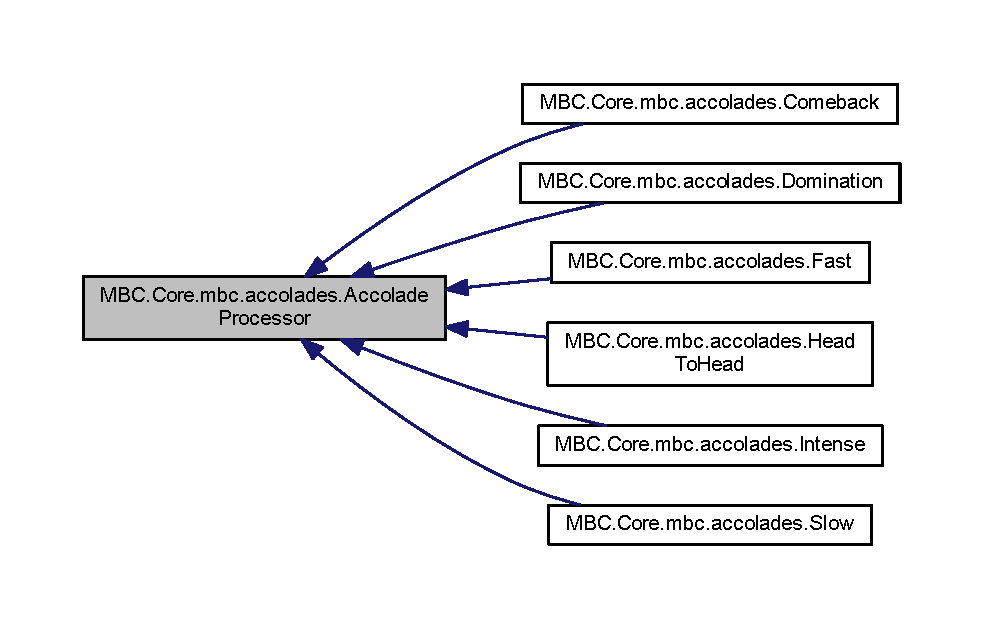
\includegraphics[width=350pt]{interface_m_b_c_1_1_core_1_1mbc_1_1accolades_1_1_accolade_processor__inherit__graph}
\end{center}
\end{figure}
\subsection*{Public Member Functions}
\begin{DoxyCompactItemize}
\item 
\hypertarget{interface_m_b_c_1_1_core_1_1mbc_1_1accolades_1_1_accolade_processor_a5c86ce623606ca27cf87ba69a753b598}{Round\-Log.\-Round\-Accolade \hyperlink{interface_m_b_c_1_1_core_1_1mbc_1_1accolades_1_1_accolade_processor_a5c86ce623606ca27cf87ba69a753b598}{Process} (\hyperlink{class_m_b_c_1_1_core_1_1_round_log_1_1_round_activity}{Round\-Log.\-Round\-Activity} a)}\label{interface_m_b_c_1_1_core_1_1mbc_1_1accolades_1_1_accolade_processor_a5c86ce623606ca27cf87ba69a753b598}

\begin{DoxyCompactList}\small\item\em Process an activity\end{DoxyCompactList}\end{DoxyCompactItemize}


The documentation for this interface was generated from the following file\-:\begin{DoxyCompactItemize}
\item 
M\-B\-C Core/accolades/Accolade\-Processor.\-cs\end{DoxyCompactItemize}

\hypertarget{class_m_b_c_1_1_w_p_f_1_1_app}{\section{M\-B\-C.\-W\-P\-F.\-App Class Reference}
\label{class_m_b_c_1_1_w_p_f_1_1_app}\index{M\-B\-C.\-W\-P\-F.\-App@{M\-B\-C.\-W\-P\-F.\-App}}
}


Interaction logic for App.\-xaml  




Inheritance diagram for M\-B\-C.\-W\-P\-F.\-App\-:
\nopagebreak
\begin{figure}[H]
\begin{center}
\leavevmode
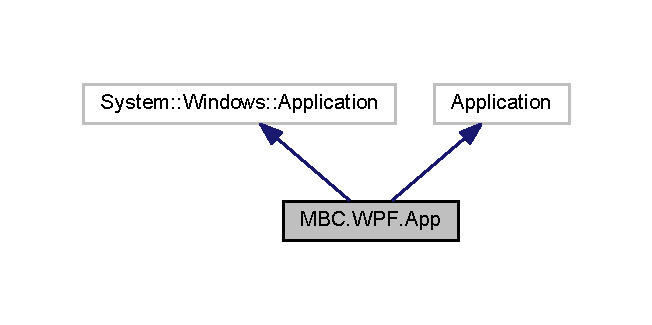
\includegraphics[width=313pt]{class_m_b_c_1_1_w_p_f_1_1_app__inherit__graph}
\end{center}
\end{figure}


Collaboration diagram for M\-B\-C.\-W\-P\-F.\-App\-:
\nopagebreak
\begin{figure}[H]
\begin{center}
\leavevmode
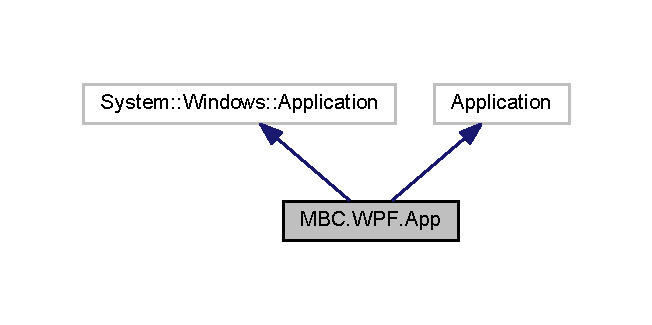
\includegraphics[width=313pt]{class_m_b_c_1_1_w_p_f_1_1_app__coll__graph}
\end{center}
\end{figure}
\subsection*{Public Member Functions}
\begin{DoxyCompactItemize}
\item 
void \hyperlink{class_m_b_c_1_1_w_p_f_1_1_app_a64e84c389e5f4a2e06725318efe701da}{Initialize\-Component} ()
\begin{DoxyCompactList}\small\item\em Initialize\-Component \end{DoxyCompactList}\end{DoxyCompactItemize}
\subsection*{Static Public Member Functions}
\begin{DoxyCompactItemize}
\item 
static void \hyperlink{class_m_b_c_1_1_w_p_f_1_1_app_aebd6635a604298686e81e5d3977fa37a}{Main} ()
\begin{DoxyCompactList}\small\item\em Application Entry Point. \end{DoxyCompactList}\end{DoxyCompactItemize}


\subsection{Detailed Description}
Interaction logic for App.\-xaml 

\hyperlink{class_m_b_c_1_1_w_p_f_1_1_app}{App} 

\subsection{Member Function Documentation}
\hypertarget{class_m_b_c_1_1_w_p_f_1_1_app_a64e84c389e5f4a2e06725318efe701da}{\index{M\-B\-C\-::\-W\-P\-F\-::\-App@{M\-B\-C\-::\-W\-P\-F\-::\-App}!Initialize\-Component@{Initialize\-Component}}
\index{Initialize\-Component@{Initialize\-Component}!MBC::WPF::App@{M\-B\-C\-::\-W\-P\-F\-::\-App}}
\subsubsection[{Initialize\-Component}]{\setlength{\rightskip}{0pt plus 5cm}void M\-B\-C.\-W\-P\-F.\-App.\-Initialize\-Component (
\begin{DoxyParamCaption}
{}
\end{DoxyParamCaption}
)}}\label{class_m_b_c_1_1_w_p_f_1_1_app_a64e84c389e5f4a2e06725318efe701da}


Initialize\-Component 

\hypertarget{class_m_b_c_1_1_w_p_f_1_1_app_aebd6635a604298686e81e5d3977fa37a}{\index{M\-B\-C\-::\-W\-P\-F\-::\-App@{M\-B\-C\-::\-W\-P\-F\-::\-App}!Main@{Main}}
\index{Main@{Main}!MBC::WPF::App@{M\-B\-C\-::\-W\-P\-F\-::\-App}}
\subsubsection[{Main}]{\setlength{\rightskip}{0pt plus 5cm}static void M\-B\-C.\-W\-P\-F.\-App.\-Main (
\begin{DoxyParamCaption}
{}
\end{DoxyParamCaption}
)\hspace{0.3cm}{\ttfamily [static]}}}\label{class_m_b_c_1_1_w_p_f_1_1_app_aebd6635a604298686e81e5d3977fa37a}


Application Entry Point. 



The documentation for this class was generated from the following files\-:\begin{DoxyCompactItemize}
\item 
M\-B\-C W\-P\-F/App.\-xaml.\-cs\item 
M\-B\-C W\-P\-F/obj/x86/\-Debug/App.\-g.\-i.\-cs\end{DoxyCompactItemize}

\hypertarget{class_m_b_c_1_1_terminal_1_1_battleship_console}{\section{M\-B\-C.\-Terminal.\-Battleship\-Console Class Reference}
\label{class_m_b_c_1_1_terminal_1_1_battleship_console}\index{M\-B\-C.\-Terminal.\-Battleship\-Console@{M\-B\-C.\-Terminal.\-Battleship\-Console}}
}


Provides an interactive console for the user. 


\subsection*{Public Member Functions}
\begin{DoxyCompactItemize}
\item 
\hypertarget{class_m_b_c_1_1_terminal_1_1_battleship_console_a1d9cdd7811c6ad93d69b64977d1670f4}{\hyperlink{class_m_b_c_1_1_terminal_1_1_battleship_console_a1d9cdd7811c6ad93d69b64977d1670f4}{Battleship\-Console} ()}\label{class_m_b_c_1_1_terminal_1_1_battleship_console_a1d9cdd7811c6ad93d69b64977d1670f4}

\begin{DoxyCompactList}\small\item\em Class constructor. Initializes the configuration object.\end{DoxyCompactList}\item 
\hypertarget{class_m_b_c_1_1_terminal_1_1_battleship_console_a24e4d77c56e575e37da9f2a7f795d2f6}{void {\bfseries Start} ()}\label{class_m_b_c_1_1_terminal_1_1_battleship_console_a24e4d77c56e575e37da9f2a7f795d2f6}

\end{DoxyCompactItemize}
\subsection*{Properties}
\begin{DoxyCompactItemize}
\item 
\hypertarget{class_m_b_c_1_1_terminal_1_1_battleship_console_a6b95099a9fb31b809a63860ba9f48867}{\hyperlink{class_m_b_c_1_1_core_1_1_configuration}{Configuration} {\bfseries Config}\hspace{0.3cm}{\ttfamily  \mbox{[}get\mbox{]}}}\label{class_m_b_c_1_1_terminal_1_1_battleship_console_a6b95099a9fb31b809a63860ba9f48867}

\end{DoxyCompactItemize}


\subsection{Detailed Description}
Provides an interactive console for the user.

The documentation for this class was generated from the following file\-:\begin{DoxyCompactItemize}
\item 
M\-B\-C Terminal/Battleship\-Console.\-cs\end{DoxyCompactItemize}

\hypertarget{class_m_b_c_1_1_core_1_1mbc_1_1accolades_1_1_comeback}{\section{M\-B\-C.\-Core.\-mbc.\-accolades.\-Comeback Class Reference}
\label{class_m_b_c_1_1_core_1_1mbc_1_1accolades_1_1_comeback}\index{M\-B\-C.\-Core.\-mbc.\-accolades.\-Comeback@{M\-B\-C.\-Core.\-mbc.\-accolades.\-Comeback}}
}


Inheritance diagram for M\-B\-C.\-Core.\-mbc.\-accolades.\-Comeback\-:\nopagebreak
\begin{figure}[H]
\begin{center}
\leavevmode
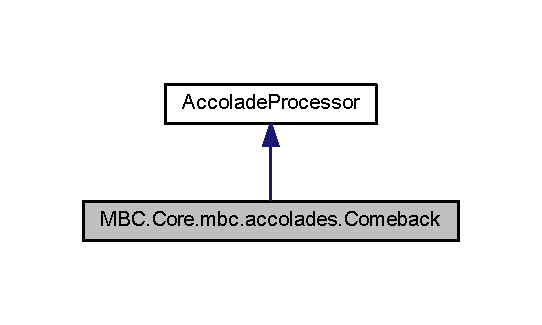
\includegraphics[width=260pt]{class_m_b_c_1_1_core_1_1mbc_1_1accolades_1_1_comeback__inherit__graph}
\end{center}
\end{figure}


Collaboration diagram for M\-B\-C.\-Core.\-mbc.\-accolades.\-Comeback\-:\nopagebreak
\begin{figure}[H]
\begin{center}
\leavevmode
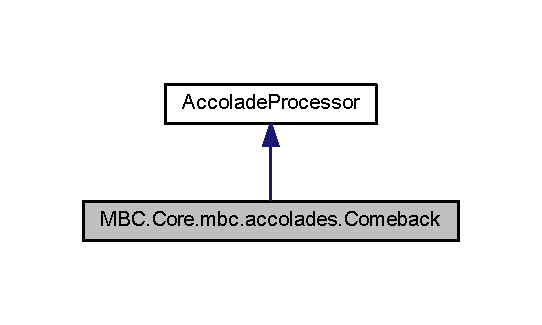
\includegraphics[width=260pt]{class_m_b_c_1_1_core_1_1mbc_1_1accolades_1_1_comeback__coll__graph}
\end{center}
\end{figure}
\subsection*{Public Member Functions}
\begin{DoxyCompactItemize}
\item 
\hypertarget{class_m_b_c_1_1_core_1_1mbc_1_1accolades_1_1_comeback_aa0df9875de35d9a73af4cde1f46c3c3b}{Round\-Log.\-Round\-Accolade \hyperlink{class_m_b_c_1_1_core_1_1mbc_1_1accolades_1_1_comeback_aa0df9875de35d9a73af4cde1f46c3c3b}{Process} (\hyperlink{class_m_b_c_1_1_core_1_1_round_log_1_1_round_activity}{Round\-Log.\-Round\-Activity} a)}\label{class_m_b_c_1_1_core_1_1mbc_1_1accolades_1_1_comeback_aa0df9875de35d9a73af4cde1f46c3c3b}

\begin{DoxyCompactList}\small\item\em Process an activity\end{DoxyCompactList}\end{DoxyCompactItemize}


The documentation for this class was generated from the following file\-:\begin{DoxyCompactItemize}
\item 
M\-B\-C Core/accolades/Comeback.\-cs\end{DoxyCompactItemize}

\hypertarget{class_m_b_c_1_1_core_1_1_competition}{\section{M\-B\-C.\-Core.\-Competition Class Reference}
\label{class_m_b_c_1_1_core_1_1_competition}\index{M\-B\-C.\-Core.\-Competition@{M\-B\-C.\-Core.\-Competition}}
}


A \hyperlink{class_m_b_c_1_1_core_1_1_competition}{Competition} object contains game logic for a game of battleship.  


\subsection*{Public Member Functions}
\begin{DoxyCompactItemize}
\item 
\hypertarget{class_m_b_c_1_1_core_1_1_competition_acfa9bb4b8a178d9981e5d4687d1487b2}{delegate void {\bfseries Rnd\-Tick} ()}\label{class_m_b_c_1_1_core_1_1_competition_acfa9bb4b8a178d9981e5d4687d1487b2}

\item 
\hypertarget{class_m_b_c_1_1_core_1_1_competition_a7378a503b4d23466fc27a2bce3ee8a37}{delegate void {\bfseries Rnd\-End} ()}\label{class_m_b_c_1_1_core_1_1_competition_a7378a503b4d23466fc27a2bce3ee8a37}

\item 
\hypertarget{class_m_b_c_1_1_core_1_1_competition_a7eecf4dc6eb7d6e7b3e6bbaf094aa1ac}{delegate void {\bfseries Match\-End} ()}\label{class_m_b_c_1_1_core_1_1_competition_a7eecf4dc6eb7d6e7b3e6bbaf094aa1ac}

\item 
\hypertarget{class_m_b_c_1_1_core_1_1_competition_ae9b5b6e7d2eedcce2956e93cafbca8ff}{\hyperlink{class_m_b_c_1_1_core_1_1_competition_ae9b5b6e7d2eedcce2956e93cafbca8ff}{Competition} (\hyperlink{interface_m_b_c_1_1_core_1_1_i_battleship_controller}{I\-Battleship\-Controller}\mbox{[}$\,$\mbox{]} ibc, \hyperlink{class_m_b_c_1_1_core_1_1_configuration}{Configuration} config)}\label{class_m_b_c_1_1_core_1_1_competition_ae9b5b6e7d2eedcce2956e93cafbca8ff}

\begin{DoxyCompactList}\small\item\em Constructs a new Battleship\-Competition object using a Battleship\-Config for configuration.\end{DoxyCompactList}\item 
\hypertarget{class_m_b_c_1_1_core_1_1_competition_a5613af0d06dd42cd00e13ed2643f88f0}{\hyperlink{class_m_b_c_1_1_core_1_1_competition_a5613af0d06dd42cd00e13ed2643f88f0}{Competition} (\hyperlink{interface_m_b_c_1_1_core_1_1_i_battleship_controller}{I\-Battleship\-Controller}\mbox{[}$\,$\mbox{]} ibc, \hyperlink{class_m_b_c_1_1_core_1_1_configuration}{Configuration} config, int seed\-Num)}\label{class_m_b_c_1_1_core_1_1_competition_a5613af0d06dd42cd00e13ed2643f88f0}

\begin{DoxyCompactList}\small\item\em Constructs a new Battleship\-Competition object using a Battleship\-Config for configuration. Also, a seed value can be specified.\end{DoxyCompactList}\item 
\hyperlink{class_m_b_c_1_1_core_1_1_field}{Field} \hyperlink{class_m_b_c_1_1_core_1_1_competition_a5e8a6b945128e37bdd87751d906edaf2}{Get\-Battlefield} ()
\item 
int \hyperlink{class_m_b_c_1_1_core_1_1_competition_a23d9364eaac330e2d3e02f28b76e3f14}{Get\-Round\-Count} ()
\item 
\hyperlink{class_m_b_c_1_1_core_1_1_round_log}{Round\-Log} \hyperlink{class_m_b_c_1_1_core_1_1_competition_a76099b9ae37d3f71c8fc54a7d34f858c}{Get\-Round\-Log\-At} (int idx)
\item 
bool \hyperlink{class_m_b_c_1_1_core_1_1_competition_adb647854be7dcd056af0200aa4693b4e}{New\-Round} ()
\begin{DoxyCompactList}\small\item\em Part of manual round control. Clears the previous round if it exists and starts a new round\end{DoxyCompactList}\item 
bool \hyperlink{class_m_b_c_1_1_core_1_1_competition_a2e64268f0a2cc09469c867b10f2ccf67}{Round\-Turn} ()
\begin{DoxyCompactList}\small\item\em Part of manual round control. Runs a turn\end{DoxyCompactList}\item 
\hypertarget{class_m_b_c_1_1_core_1_1_competition_af2375ef2193559c123404a78fa7cf1a4}{void \hyperlink{class_m_b_c_1_1_core_1_1_competition_af2375ef2193559c123404a78fa7cf1a4}{Run\-Round} ()}\label{class_m_b_c_1_1_core_1_1_competition_af2375ef2193559c123404a78fa7cf1a4}

\begin{DoxyCompactList}\small\item\em Runs an entire round until an opponent wins\end{DoxyCompactList}\item 
\hypertarget{class_m_b_c_1_1_core_1_1_competition_ad235bc0d31dc88cfb661278d0613ec08}{Dictionary\\*
$<$ \hyperlink{interface_m_b_c_1_1_core_1_1_i_battleship_controller}{I\-Battleship\-Controller}, int $>$ \hyperlink{class_m_b_c_1_1_core_1_1_competition_ad235bc0d31dc88cfb661278d0613ec08}{Get\-Scores} ()}\label{class_m_b_c_1_1_core_1_1_competition_ad235bc0d31dc88cfb661278d0613ec08}

\begin{DoxyCompactList}\small\item\em Returns a dictionary linking the scores to the opponents.\end{DoxyCompactList}\item 
void \hyperlink{class_m_b_c_1_1_core_1_1_competition_ae6f1520c4f77bef9f8b9760b40517857}{Run\-Rounds} (int rnds, bool play\-Out)
\begin{DoxyCompactList}\small\item\em Runs a specified amount of rounds between two opponents.\end{DoxyCompactList}\item 
\hypertarget{class_m_b_c_1_1_core_1_1_competition_a4b22f726ea27bfb57696f3a92a6677af}{void \hyperlink{class_m_b_c_1_1_core_1_1_competition_a4b22f726ea27bfb57696f3a92a6677af}{Run\-Competition} ()}\label{class_m_b_c_1_1_core_1_1_competition_a4b22f726ea27bfb57696f3a92a6677af}

\begin{DoxyCompactList}\small\item\em Runs the match between two opponents. Bases the amount of rounds to play and how to play them in the configuration.\end{DoxyCompactList}\item 
\hypertarget{class_m_b_c_1_1_core_1_1_competition_aa44653a37635021dadc6d5e60b8815a5}{void \hyperlink{class_m_b_c_1_1_core_1_1_competition_aa44653a37635021dadc6d5e60b8815a5}{Run\-Competition\-Thread} ()}\label{class_m_b_c_1_1_core_1_1_competition_aa44653a37635021dadc6d5e60b8815a5}

\begin{DoxyCompactList}\small\item\em Runs the match between two opponents in a separate thread using the configuration.\end{DoxyCompactList}\item 
\hypertarget{class_m_b_c_1_1_core_1_1_competition_a45faa0917180f6a7b3520e5fedc35d9e}{void \hyperlink{class_m_b_c_1_1_core_1_1_competition_a45faa0917180f6a7b3520e5fedc35d9e}{Stop\-Competition\-Thread} ()}\label{class_m_b_c_1_1_core_1_1_competition_a45faa0917180f6a7b3520e5fedc35d9e}

\begin{DoxyCompactList}\small\item\em Stops rounds from being played anymore.\end{DoxyCompactList}\end{DoxyCompactItemize}
\subsection*{Static Public Member Functions}
\begin{DoxyCompactItemize}
\item 
\hypertarget{class_m_b_c_1_1_core_1_1_competition_acf765bf2efdcb823da7a7e164b316ce7}{static void \hyperlink{class_m_b_c_1_1_core_1_1_competition_acf765bf2efdcb823da7a7e164b316ce7}{Set\-Config\-Defaults} ()}\label{class_m_b_c_1_1_core_1_1_competition_acf765bf2efdcb823da7a7e164b316ce7}

\begin{DoxyCompactList}\small\item\em Sets default configuration values for keys that relate to this class. Should be called before using the global \hyperlink{class_m_b_c_1_1_core_1_1_configuration_a5db184730b6c51c2ae617d0fc1976c13}{Configuration.\-Default} object.\end{DoxyCompactList}\end{DoxyCompactItemize}
\subsection*{Events}
\begin{DoxyCompactItemize}
\item 
\hypertarget{class_m_b_c_1_1_core_1_1_competition_ab7b3837c19e15f934e926a0c7664c9b1}{Rnd\-Tick {\bfseries Round\-Turn\-End\-Event}}\label{class_m_b_c_1_1_core_1_1_competition_ab7b3837c19e15f934e926a0c7664c9b1}

\item 
\hypertarget{class_m_b_c_1_1_core_1_1_competition_adf9afeb254a4b862106613a6301d4f8e}{Rnd\-End {\bfseries Round\-End\-Event}}\label{class_m_b_c_1_1_core_1_1_competition_adf9afeb254a4b862106613a6301d4f8e}

\item 
\hypertarget{class_m_b_c_1_1_core_1_1_competition_a0188f6329f06caaf50efc3fc3914d9b5}{Match\-End {\bfseries Match\-End\-Event}}\label{class_m_b_c_1_1_core_1_1_competition_a0188f6329f06caaf50efc3fc3914d9b5}

\end{DoxyCompactItemize}


\subsection{Detailed Description}
A \hyperlink{class_m_b_c_1_1_core_1_1_competition}{Competition} object contains game logic for a game of battleship. 

A competition has 3 events that are called internally during game play\-: \begin{DoxyVerb} RoundTurnEndEvent - Called when a controller has ended their turn.
 RoundEndEvent - Called when a round has ended.
 MatchEndEvent - Called when a matchup has ended (from any methods invoking RunRounds)
\end{DoxyVerb}


The competition can be run either in the same thread as the calling method (\hyperlink{class_m_b_c_1_1_core_1_1_competition_a4b22f726ea27bfb57696f3a92a6677af}{Run\-Competition()}), or in a different thread (\hyperlink{class_m_b_c_1_1_core_1_1_competition_aa44653a37635021dadc6d5e60b8815a5}{Run\-Competition\-Thread()}), which can be stopped at any time (\hyperlink{class_m_b_c_1_1_core_1_1_competition_a45faa0917180f6a7b3520e5fedc35d9e}{Stop\-Competition\-Thread()}). By using one of these methods, the \hyperlink{class_m_b_c_1_1_core_1_1_competition}{Competition} object will use the \hyperlink{class_m_b_c_1_1_core_1_1_configuration}{Configuration} object that it has been constructed with to determine the number of rounds to play. Using \hyperlink{class_m_b_c_1_1_core_1_1_competition_ae6f1520c4f77bef9f8b9760b40517857}{Run\-Rounds(int, bool)} will run a custom number of rounds in the same thread, but use of this method is not recommended.

The competition can be run in a turn-\/by-\/turn manner by utilizing three methods\-: \begin{DoxyVerb} NewRound() - Starts a new round in the competition. Finishes any ongoing round.
 RoundTurn() - Run a turn in the round.
 RoundRun() - Run through remaining turns in the round.
\end{DoxyVerb}


When constructing a new \hyperlink{class_m_b_c_1_1_core_1_1_competition}{Competition}, keep in mind that the order of the array of I\-Battleship\-Controllers does not change, even in the \hyperlink{class_m_b_c_1_1_core_1_1_field}{Field} object that is generated. 

\subsection{Member Function Documentation}
\hypertarget{class_m_b_c_1_1_core_1_1_competition_a5e8a6b945128e37bdd87751d906edaf2}{\index{M\-B\-C\-::\-Core\-::\-Competition@{M\-B\-C\-::\-Core\-::\-Competition}!Get\-Battlefield@{Get\-Battlefield}}
\index{Get\-Battlefield@{Get\-Battlefield}!MBC::Core::Competition@{M\-B\-C\-::\-Core\-::\-Competition}}
\subsubsection[{Get\-Battlefield}]{\setlength{\rightskip}{0pt plus 5cm}{\bf Field} M\-B\-C.\-Core.\-Competition.\-Get\-Battlefield (
\begin{DoxyParamCaption}
{}
\end{DoxyParamCaption}
)}}\label{class_m_b_c_1_1_core_1_1_competition_a5e8a6b945128e37bdd87751d906edaf2}
\begin{DoxyReturn}{Returns}
The battlefield associated with this competition
\end{DoxyReturn}
\hypertarget{class_m_b_c_1_1_core_1_1_competition_a23d9364eaac330e2d3e02f28b76e3f14}{\index{M\-B\-C\-::\-Core\-::\-Competition@{M\-B\-C\-::\-Core\-::\-Competition}!Get\-Round\-Count@{Get\-Round\-Count}}
\index{Get\-Round\-Count@{Get\-Round\-Count}!MBC::Core::Competition@{M\-B\-C\-::\-Core\-::\-Competition}}
\subsubsection[{Get\-Round\-Count}]{\setlength{\rightskip}{0pt plus 5cm}int M\-B\-C.\-Core.\-Competition.\-Get\-Round\-Count (
\begin{DoxyParamCaption}
{}
\end{DoxyParamCaption}
)}}\label{class_m_b_c_1_1_core_1_1_competition_a23d9364eaac330e2d3e02f28b76e3f14}
\begin{DoxyReturn}{Returns}
The number of rounds played, complete or incomplete
\end{DoxyReturn}
\hypertarget{class_m_b_c_1_1_core_1_1_competition_a76099b9ae37d3f71c8fc54a7d34f858c}{\index{M\-B\-C\-::\-Core\-::\-Competition@{M\-B\-C\-::\-Core\-::\-Competition}!Get\-Round\-Log\-At@{Get\-Round\-Log\-At}}
\index{Get\-Round\-Log\-At@{Get\-Round\-Log\-At}!MBC::Core::Competition@{M\-B\-C\-::\-Core\-::\-Competition}}
\subsubsection[{Get\-Round\-Log\-At}]{\setlength{\rightskip}{0pt plus 5cm}{\bf Round\-Log} M\-B\-C.\-Core.\-Competition.\-Get\-Round\-Log\-At (
\begin{DoxyParamCaption}
\item[{int}]{idx}
\end{DoxyParamCaption}
)}}\label{class_m_b_c_1_1_core_1_1_competition_a76099b9ae37d3f71c8fc54a7d34f858c}
\begin{DoxyReturn}{Returns}
The log for the round \#idx
\end{DoxyReturn}
\hypertarget{class_m_b_c_1_1_core_1_1_competition_adb647854be7dcd056af0200aa4693b4e}{\index{M\-B\-C\-::\-Core\-::\-Competition@{M\-B\-C\-::\-Core\-::\-Competition}!New\-Round@{New\-Round}}
\index{New\-Round@{New\-Round}!MBC::Core::Competition@{M\-B\-C\-::\-Core\-::\-Competition}}
\subsubsection[{New\-Round}]{\setlength{\rightskip}{0pt plus 5cm}bool M\-B\-C.\-Core.\-Competition.\-New\-Round (
\begin{DoxyParamCaption}
{}
\end{DoxyParamCaption}
)}}\label{class_m_b_c_1_1_core_1_1_competition_adb647854be7dcd056af0200aa4693b4e}


Part of manual round control. Clears the previous round if it exists and starts a new round

\begin{DoxyReturn}{Returns}
True if the round is ongoing, false if it has been won
\end{DoxyReturn}
\hypertarget{class_m_b_c_1_1_core_1_1_competition_a2e64268f0a2cc09469c867b10f2ccf67}{\index{M\-B\-C\-::\-Core\-::\-Competition@{M\-B\-C\-::\-Core\-::\-Competition}!Round\-Turn@{Round\-Turn}}
\index{Round\-Turn@{Round\-Turn}!MBC::Core::Competition@{M\-B\-C\-::\-Core\-::\-Competition}}
\subsubsection[{Round\-Turn}]{\setlength{\rightskip}{0pt plus 5cm}bool M\-B\-C.\-Core.\-Competition.\-Round\-Turn (
\begin{DoxyParamCaption}
{}
\end{DoxyParamCaption}
)}}\label{class_m_b_c_1_1_core_1_1_competition_a2e64268f0a2cc09469c867b10f2ccf67}


Part of manual round control. Runs a turn

\begin{DoxyReturn}{Returns}
True if the round is still ongoing, false if the round is finished
\end{DoxyReturn}
\hypertarget{class_m_b_c_1_1_core_1_1_competition_ae6f1520c4f77bef9f8b9760b40517857}{\index{M\-B\-C\-::\-Core\-::\-Competition@{M\-B\-C\-::\-Core\-::\-Competition}!Run\-Rounds@{Run\-Rounds}}
\index{Run\-Rounds@{Run\-Rounds}!MBC::Core::Competition@{M\-B\-C\-::\-Core\-::\-Competition}}
\subsubsection[{Run\-Rounds}]{\setlength{\rightskip}{0pt plus 5cm}void M\-B\-C.\-Core.\-Competition.\-Run\-Rounds (
\begin{DoxyParamCaption}
\item[{int}]{rnds, }
\item[{bool}]{play\-Out}
\end{DoxyParamCaption}
)}}\label{class_m_b_c_1_1_core_1_1_competition_ae6f1520c4f77bef9f8b9760b40517857}


Runs a specified amount of rounds between two opponents.

\begin{DoxyReturn}{Returns}
A list of the two opponents with their scores attached.
\end{DoxyReturn}

\begin{DoxyParams}{Parameters}
{\em play\-Out} & If the amount of rounds specified is to be played out (ie. total score between the two opponents) or not (ie. first score to rounds)\\
\hline
{\em rnds} & The amount of rounds to play.\\
\hline
\end{DoxyParams}


Here is the call graph for this function\-:
\nopagebreak
\begin{figure}[H]
\begin{center}
\leavevmode
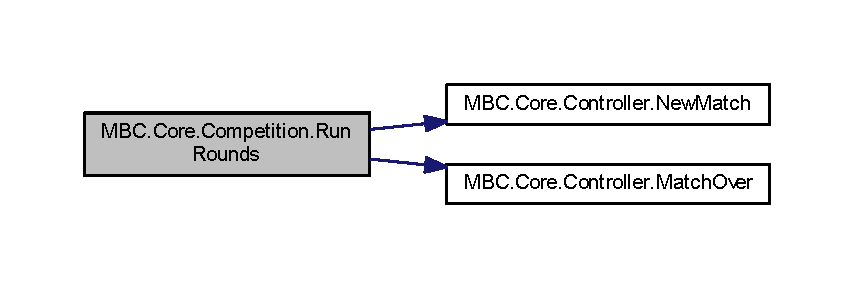
\includegraphics[width=350pt]{class_m_b_c_1_1_core_1_1_competition_ae6f1520c4f77bef9f8b9760b40517857_cgraph}
\end{center}
\end{figure}




The documentation for this class was generated from the following file\-:\begin{DoxyCompactItemize}
\item 
Core/Competition.\-cs\end{DoxyCompactItemize}

\hypertarget{class_m_b_c_1_1_terminal_1_1_competition_state}{\section{M\-B\-C.\-Terminal.\-Competition\-State Class Reference}
\label{class_m_b_c_1_1_terminal_1_1_competition_state}\index{M\-B\-C.\-Terminal.\-Competition\-State@{M\-B\-C.\-Terminal.\-Competition\-State}}
}


Inheritance diagram for M\-B\-C.\-Terminal.\-Competition\-State\-:\nopagebreak
\begin{figure}[H]
\begin{center}
\leavevmode
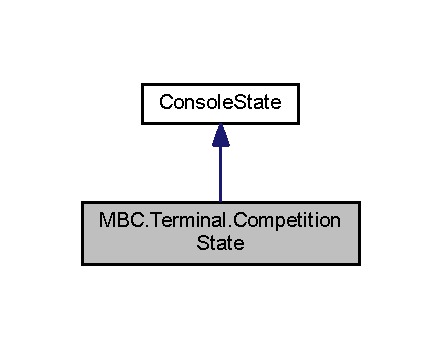
\includegraphics[width=212pt]{class_m_b_c_1_1_terminal_1_1_competition_state__inherit__graph}
\end{center}
\end{figure}


Collaboration diagram for M\-B\-C.\-Terminal.\-Competition\-State\-:\nopagebreak
\begin{figure}[H]
\begin{center}
\leavevmode
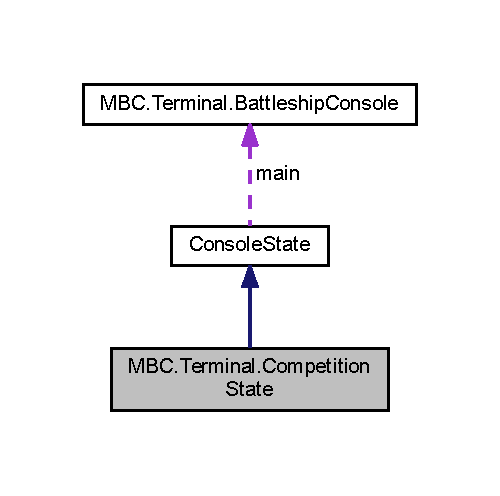
\includegraphics[width=240pt]{class_m_b_c_1_1_terminal_1_1_competition_state__coll__graph}
\end{center}
\end{figure}
\subsection*{Public Member Functions}
\begin{DoxyCompactItemize}
\item 
\hypertarget{class_m_b_c_1_1_terminal_1_1_competition_state_a30f9e150db2d951fc3844d9bb4d575c8}{{\bfseries Competition\-State} (\hyperlink{class_m_b_c_1_1_terminal_1_1_battleship_console}{Battleship\-Console} main, \hyperlink{interface_m_b_c_1_1_core_1_1_i_battleship_controller}{I\-Battleship\-Controller}\mbox{[}$\,$\mbox{]} ibc)}\label{class_m_b_c_1_1_terminal_1_1_competition_state_a30f9e150db2d951fc3844d9bb4d575c8}

\end{DoxyCompactItemize}
\subsection*{Protected Member Functions}
\begin{DoxyCompactItemize}
\item 
\hypertarget{class_m_b_c_1_1_terminal_1_1_competition_state_a910a4059941eca78c26368f33fc7ba40}{override void \hyperlink{class_m_b_c_1_1_terminal_1_1_competition_state_a910a4059941eca78c26368f33fc7ba40}{State\-Display} ()}\label{class_m_b_c_1_1_terminal_1_1_competition_state_a910a4059941eca78c26368f33fc7ba40}

\begin{DoxyCompactList}\small\item\em Overridden to provide specific printing related to the subclass.\end{DoxyCompactList}\item 
override \hyperlink{class_m_b_c_1_1_terminal_1_1_console_state}{Console\-State} \hyperlink{class_m_b_c_1_1_terminal_1_1_competition_state_a85808b20e9ecb90e400eb6dcbb5929fd}{Response} (string input)
\begin{DoxyCompactList}\small\item\em Called when input is not handled by the base class.\end{DoxyCompactList}\end{DoxyCompactItemize}
\subsection*{Additional Inherited Members}


\subsection{Member Function Documentation}
\hypertarget{class_m_b_c_1_1_terminal_1_1_competition_state_a85808b20e9ecb90e400eb6dcbb5929fd}{\index{M\-B\-C\-::\-Terminal\-::\-Competition\-State@{M\-B\-C\-::\-Terminal\-::\-Competition\-State}!Response@{Response}}
\index{Response@{Response}!MBC::Terminal::CompetitionState@{M\-B\-C\-::\-Terminal\-::\-Competition\-State}}
\subsubsection[{Response}]{\setlength{\rightskip}{0pt plus 5cm}override {\bf Console\-State} M\-B\-C.\-Terminal.\-Competition\-State.\-Response (
\begin{DoxyParamCaption}
\item[{string}]{input}
\end{DoxyParamCaption}
)\hspace{0.3cm}{\ttfamily [protected]}, {\ttfamily [virtual]}}}\label{class_m_b_c_1_1_terminal_1_1_competition_state_a85808b20e9ecb90e400eb6dcbb5929fd}


Called when input is not handled by the base class.


\begin{DoxyParams}{Parameters}
{\em input} & The string entered by the user\\
\hline
\end{DoxyParams}
\begin{DoxyReturn}{Returns}
The implementing class, null, or a new \hyperlink{class_m_b_c_1_1_terminal_1_1_console_state}{Console\-State} object. null will end the program.
\end{DoxyReturn}


Implements \hyperlink{class_m_b_c_1_1_terminal_1_1_console_state_a93d6eee582913a59d10348cdc8ef4248}{M\-B\-C.\-Terminal.\-Console\-State}.



The documentation for this class was generated from the following file\-:\begin{DoxyCompactItemize}
\item 
M\-B\-C Terminal/Competition\-State.\-cs\end{DoxyCompactItemize}

\hypertarget{class_m_b_c_1_1_core_1_1_configuration}{\section{M\-B\-C.\-Core.\-Configuration Class Reference}
\label{class_m_b_c_1_1_core_1_1_configuration}\index{M\-B\-C.\-Core.\-Configuration@{M\-B\-C.\-Core.\-Configuration}}
}


Battleship\-Config deals with a single configuration file and parses each key/value pair. 


\subsection*{Public Member Functions}
\begin{DoxyCompactItemize}
\item 
\hypertarget{class_m_b_c_1_1_core_1_1_configuration_aa0551a9f6fc9d76aa2300da55f6ea135}{\hyperlink{class_m_b_c_1_1_core_1_1_configuration_aa0551a9f6fc9d76aa2300da55f6ea135}{Configuration} (string name)}\label{class_m_b_c_1_1_core_1_1_configuration_aa0551a9f6fc9d76aa2300da55f6ea135}

\begin{DoxyCompactList}\small\item\em Initializes this Battleship\-Config by loading from a config file. If it does not exist, then it loads the default values.\end{DoxyCompactList}\item 
\hypertarget{class_m_b_c_1_1_core_1_1_configuration_a7fd9b75ad6dcea3175cd25e4afe9f59e}{void \hyperlink{class_m_b_c_1_1_core_1_1_configuration_a7fd9b75ad6dcea3175cd25e4afe9f59e}{Rename} (string new\-Name)}\label{class_m_b_c_1_1_core_1_1_configuration_a7fd9b75ad6dcea3175cd25e4afe9f59e}

\begin{DoxyCompactList}\small\item\em Renames this configuration file for file input or output\end{DoxyCompactList}\item 
T \hyperlink{class_m_b_c_1_1_core_1_1_configuration_addce147239dffada4ca7bb0c8a0b7522}{Get\-Value$<$ T $>$} (string s)
\begin{DoxyCompactList}\small\item\em Gets a value from the configuration\end{DoxyCompactList}\item 
\hypertarget{class_m_b_c_1_1_core_1_1_configuration_a4f161db0d533cac5ddbf558fa2aaea3b}{void \hyperlink{class_m_b_c_1_1_core_1_1_configuration_a4f161db0d533cac5ddbf558fa2aaea3b}{Set\-Value$<$ T $>$} (string s, T val)}\label{class_m_b_c_1_1_core_1_1_configuration_a4f161db0d533cac5ddbf558fa2aaea3b}

\begin{DoxyCompactList}\small\item\em Sets a value in the configuration\end{DoxyCompactList}\item 
List$<$ T $>$ \hyperlink{class_m_b_c_1_1_core_1_1_configuration_a99b689b17905c31fa760cc92ceb2fa89}{Get\-Config\-Value\-Array$<$ T $>$} (string s)
\begin{DoxyCompactList}\small\item\em Gets a comma-\/delimited array (list) from the configuration\end{DoxyCompactList}\item 
void \hyperlink{class_m_b_c_1_1_core_1_1_configuration_a04f21c72d510c6486acfc8c27fdc34ce}{Save\-Config\-File} ()
\begin{DoxyCompactList}\small\item\em Saves the current configuration to a file.\end{DoxyCompactList}\end{DoxyCompactItemize}
\subsection*{Static Public Member Functions}
\begin{DoxyCompactItemize}
\item 
static List$<$ string $>$ \hyperlink{class_m_b_c_1_1_core_1_1_configuration_a6b5833220d539c7b7e48863659bd1cde}{Get\-Available\-Configs} ()
\end{DoxyCompactItemize}
\subsection*{Properties}
\begin{DoxyCompactItemize}
\item 
\hypertarget{class_m_b_c_1_1_core_1_1_configuration_a4f09a03f95c3beaa3ae10c3ae7aa7624}{static \hyperlink{class_m_b_c_1_1_core_1_1_configuration}{Configuration} \hyperlink{class_m_b_c_1_1_core_1_1_configuration_a4f09a03f95c3beaa3ae10c3ae7aa7624}{Global}\hspace{0.3cm}{\ttfamily  \mbox{[}get\mbox{]}}}\label{class_m_b_c_1_1_core_1_1_configuration_a4f09a03f95c3beaa3ae10c3ae7aa7624}

\begin{DoxyCompactList}\small\item\em Gets a common configuration object for use.\end{DoxyCompactList}\item 
\hypertarget{class_m_b_c_1_1_core_1_1_configuration_a5db184730b6c51c2ae617d0fc1976c13}{static \hyperlink{class_m_b_c_1_1_core_1_1_configuration}{Configuration} \hyperlink{class_m_b_c_1_1_core_1_1_configuration_a5db184730b6c51c2ae617d0fc1976c13}{Default}\hspace{0.3cm}{\ttfamily  \mbox{[}get\mbox{]}}}\label{class_m_b_c_1_1_core_1_1_configuration_a5db184730b6c51c2ae617d0fc1976c13}

\begin{DoxyCompactList}\small\item\em Gets the default configuration. Used to set the default values for the \end{DoxyCompactList}\end{DoxyCompactItemize}


\subsection{Detailed Description}
Battleship\-Config deals with a single configuration file and parses each key/value pair.

\subsection{Member Function Documentation}
\hypertarget{class_m_b_c_1_1_core_1_1_configuration_a6b5833220d539c7b7e48863659bd1cde}{\index{M\-B\-C\-::\-Core\-::\-Configuration@{M\-B\-C\-::\-Core\-::\-Configuration}!Get\-Available\-Configs@{Get\-Available\-Configs}}
\index{Get\-Available\-Configs@{Get\-Available\-Configs}!MBC::Core::Configuration@{M\-B\-C\-::\-Core\-::\-Configuration}}
\subsubsection[{Get\-Available\-Configs}]{\setlength{\rightskip}{0pt plus 5cm}static List$<$string$>$ M\-B\-C.\-Core.\-Configuration.\-Get\-Available\-Configs (
\begin{DoxyParamCaption}
{}
\end{DoxyParamCaption}
)\hspace{0.3cm}{\ttfamily [static]}}}\label{class_m_b_c_1_1_core_1_1_configuration_a6b5833220d539c7b7e48863659bd1cde}
\begin{DoxyReturn}{Returns}
The names of existing configuration files
\end{DoxyReturn}
\hypertarget{class_m_b_c_1_1_core_1_1_configuration_a99b689b17905c31fa760cc92ceb2fa89}{\index{M\-B\-C\-::\-Core\-::\-Configuration@{M\-B\-C\-::\-Core\-::\-Configuration}!Get\-Config\-Value\-Array$<$ T $>$@{Get\-Config\-Value\-Array$<$ T $>$}}
\index{Get\-Config\-Value\-Array$<$ T $>$@{Get\-Config\-Value\-Array$<$ T $>$}!MBC::Core::Configuration@{M\-B\-C\-::\-Core\-::\-Configuration}}
\subsubsection[{Get\-Config\-Value\-Array$<$ T $>$}]{\setlength{\rightskip}{0pt plus 5cm}List$<$T$>$ M\-B\-C.\-Core.\-Configuration.\-Get\-Config\-Value\-Array$<$ T $>$ (
\begin{DoxyParamCaption}
\item[{string}]{s}
\end{DoxyParamCaption}
)}}\label{class_m_b_c_1_1_core_1_1_configuration_a99b689b17905c31fa760cc92ceb2fa89}


Gets a comma-\/delimited array (list) from the configuration


\begin{DoxyParams}{Parameters}
{\em s} & The key to get the value from\\
\hline
{\em def} & The default value for a given key if the key is not found.\\
\hline
\end{DoxyParams}
\begin{DoxyReturn}{Returns}
The list loaded from the configuration, otherwise, the default value
\end{DoxyReturn}
\hypertarget{class_m_b_c_1_1_core_1_1_configuration_addce147239dffada4ca7bb0c8a0b7522}{\index{M\-B\-C\-::\-Core\-::\-Configuration@{M\-B\-C\-::\-Core\-::\-Configuration}!Get\-Value$<$ T $>$@{Get\-Value$<$ T $>$}}
\index{Get\-Value$<$ T $>$@{Get\-Value$<$ T $>$}!MBC::Core::Configuration@{M\-B\-C\-::\-Core\-::\-Configuration}}
\subsubsection[{Get\-Value$<$ T $>$}]{\setlength{\rightskip}{0pt plus 5cm}T M\-B\-C.\-Core.\-Configuration.\-Get\-Value$<$ T $>$ (
\begin{DoxyParamCaption}
\item[{string}]{s}
\end{DoxyParamCaption}
)}}\label{class_m_b_c_1_1_core_1_1_configuration_addce147239dffada4ca7bb0c8a0b7522}


Gets a value from the configuration


\begin{DoxyParams}{Parameters}
{\em s} & The key to get the value from\\
\hline
{\em def} & The default value for a given key if the key is not found.\\
\hline
\end{DoxyParams}
\begin{DoxyReturn}{Returns}
The value loaded from the configuration, otherwise, the default value.
\end{DoxyReturn}
\hypertarget{class_m_b_c_1_1_core_1_1_configuration_a04f21c72d510c6486acfc8c27fdc34ce}{\index{M\-B\-C\-::\-Core\-::\-Configuration@{M\-B\-C\-::\-Core\-::\-Configuration}!Save\-Config\-File@{Save\-Config\-File}}
\index{Save\-Config\-File@{Save\-Config\-File}!MBC::Core::Configuration@{M\-B\-C\-::\-Core\-::\-Configuration}}
\subsubsection[{Save\-Config\-File}]{\setlength{\rightskip}{0pt plus 5cm}void M\-B\-C.\-Core.\-Configuration.\-Save\-Config\-File (
\begin{DoxyParamCaption}
{}
\end{DoxyParamCaption}
)}}\label{class_m_b_c_1_1_core_1_1_configuration_a04f21c72d510c6486acfc8c27fdc34ce}


Saves the current configuration to a file.


\begin{DoxyExceptions}{Exceptions}
{\em I\-O\-Exception} & The file could not be written to.\\
\hline
\end{DoxyExceptions}


The documentation for this class was generated from the following file\-:\begin{DoxyCompactItemize}
\item 
M\-B\-C Core/util/Configuration.\-cs\end{DoxyCompactItemize}

\hypertarget{class_m_b_c_1_1_terminal_1_1_console_state}{\section{M\-B\-C.\-Terminal.\-Console\-State Class Reference}
\label{class_m_b_c_1_1_terminal_1_1_console_state}\index{M\-B\-C.\-Terminal.\-Console\-State@{M\-B\-C.\-Terminal.\-Console\-State}}
}


The base class for console states 




Inheritance diagram for M\-B\-C.\-Terminal.\-Console\-State\-:\nopagebreak
\begin{figure}[H]
\begin{center}
\leavevmode
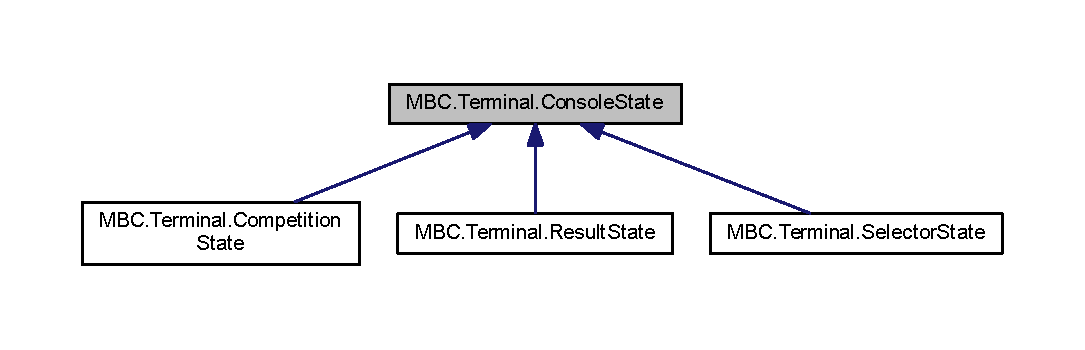
\includegraphics[width=350pt]{class_m_b_c_1_1_terminal_1_1_console_state__inherit__graph}
\end{center}
\end{figure}


Collaboration diagram for M\-B\-C.\-Terminal.\-Console\-State\-:\nopagebreak
\begin{figure}[H]
\begin{center}
\leavevmode
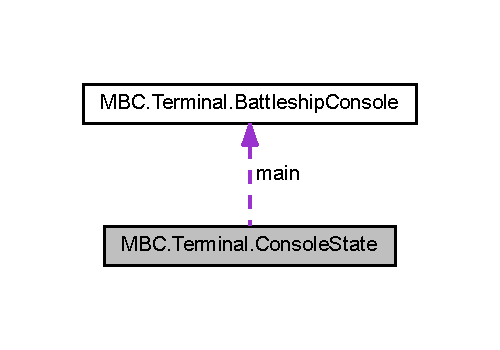
\includegraphics[width=240pt]{class_m_b_c_1_1_terminal_1_1_console_state__coll__graph}
\end{center}
\end{figure}
\subsection*{Public Member Functions}
\begin{DoxyCompactItemize}
\item 
\hypertarget{class_m_b_c_1_1_terminal_1_1_console_state_a43411c7f185d916c492ba60be49f6a50}{{\bfseries Console\-State} (\hyperlink{class_m_b_c_1_1_terminal_1_1_battleship_console}{Battleship\-Console} main)}\label{class_m_b_c_1_1_terminal_1_1_console_state_a43411c7f185d916c492ba60be49f6a50}

\item 
\hyperlink{class_m_b_c_1_1_terminal_1_1_console_state}{Console\-State} \hyperlink{class_m_b_c_1_1_terminal_1_1_console_state_a3ecdb3a79aec98954b866c125101904e}{Get\-Input} (string input)
\begin{DoxyCompactList}\small\item\em Called in the loop, used for input interactivity.\end{DoxyCompactList}\item 
void \hyperlink{class_m_b_c_1_1_terminal_1_1_console_state_a91b990b98bcf47af6a134dd8353477bf}{Write\-Centered\-Text} (string text, string ends)
\begin{DoxyCompactList}\small\item\em Prints the specified text, with the specified ends, centered, to the console.\end{DoxyCompactList}\item 
\hypertarget{class_m_b_c_1_1_terminal_1_1_console_state_ad76828bd874ddb99b7c2ca29a4291f7a}{void \hyperlink{class_m_b_c_1_1_terminal_1_1_console_state_ad76828bd874ddb99b7c2ca29a4291f7a}{Display} ()}\label{class_m_b_c_1_1_terminal_1_1_console_state_ad76828bd874ddb99b7c2ca29a4291f7a}

\begin{DoxyCompactList}\small\item\em Called in the loop, this provides a standard way for user interactivity and display.\end{DoxyCompactList}\end{DoxyCompactItemize}
\subsection*{Protected Member Functions}
\begin{DoxyCompactItemize}
\item 
void \hyperlink{class_m_b_c_1_1_terminal_1_1_console_state_a8979ac7d7e895a6eff290b39166acee8}{Write\-Chars} (char c, int n)
\begin{DoxyCompactList}\small\item\em Writes a specific character for a number of times.\end{DoxyCompactList}\item 
\hypertarget{class_m_b_c_1_1_terminal_1_1_console_state_acd7345ff099de65c8930ff4a77fc0fa9}{abstract void \hyperlink{class_m_b_c_1_1_terminal_1_1_console_state_acd7345ff099de65c8930ff4a77fc0fa9}{State\-Display} ()}\label{class_m_b_c_1_1_terminal_1_1_console_state_acd7345ff099de65c8930ff4a77fc0fa9}

\begin{DoxyCompactList}\small\item\em Overridden to provide specific printing related to the subclass.\end{DoxyCompactList}\item 
abstract \hyperlink{class_m_b_c_1_1_terminal_1_1_console_state}{Console\-State} \hyperlink{class_m_b_c_1_1_terminal_1_1_console_state_a93d6eee582913a59d10348cdc8ef4248}{Response} (string input)
\begin{DoxyCompactList}\small\item\em Called when input is not handled by the base class.\end{DoxyCompactList}\end{DoxyCompactItemize}
\subsection*{Protected Attributes}
\begin{DoxyCompactItemize}
\item 
\hypertarget{class_m_b_c_1_1_terminal_1_1_console_state_a50ec0fffe2fc39dfa2432e568c8cb3bc}{\hyperlink{class_m_b_c_1_1_terminal_1_1_battleship_console}{Battleship\-Console} {\bfseries main}}\label{class_m_b_c_1_1_terminal_1_1_console_state_a50ec0fffe2fc39dfa2432e568c8cb3bc}

\item 
\hypertarget{class_m_b_c_1_1_terminal_1_1_console_state_a89c588675d6b388380eb66321cc14413}{string {\bfseries extra\-Menu} = \char`\"{}\char`\"{}}\label{class_m_b_c_1_1_terminal_1_1_console_state_a89c588675d6b388380eb66321cc14413}

\item 
\hypertarget{class_m_b_c_1_1_terminal_1_1_console_state_adcf09c50ab0b287fe774626c0697a8f3}{const string {\bfseries header\-Ends} = \char`\"{}=====================\char`\"{}}\label{class_m_b_c_1_1_terminal_1_1_console_state_adcf09c50ab0b287fe774626c0697a8f3}

\end{DoxyCompactItemize}


\subsection{Detailed Description}
The base class for console states

\subsection{Member Function Documentation}
\hypertarget{class_m_b_c_1_1_terminal_1_1_console_state_a3ecdb3a79aec98954b866c125101904e}{\index{M\-B\-C\-::\-Terminal\-::\-Console\-State@{M\-B\-C\-::\-Terminal\-::\-Console\-State}!Get\-Input@{Get\-Input}}
\index{Get\-Input@{Get\-Input}!MBC::Terminal::ConsoleState@{M\-B\-C\-::\-Terminal\-::\-Console\-State}}
\subsubsection[{Get\-Input}]{\setlength{\rightskip}{0pt plus 5cm}{\bf Console\-State} M\-B\-C.\-Terminal.\-Console\-State.\-Get\-Input (
\begin{DoxyParamCaption}
\item[{string}]{input}
\end{DoxyParamCaption}
)}}\label{class_m_b_c_1_1_terminal_1_1_console_state_a3ecdb3a79aec98954b866c125101904e}


Called in the loop, used for input interactivity.


\begin{DoxyParams}{Parameters}
{\em input} & The string entered by the user into the console\\
\hline
\end{DoxyParams}
\hypertarget{class_m_b_c_1_1_terminal_1_1_console_state_a93d6eee582913a59d10348cdc8ef4248}{\index{M\-B\-C\-::\-Terminal\-::\-Console\-State@{M\-B\-C\-::\-Terminal\-::\-Console\-State}!Response@{Response}}
\index{Response@{Response}!MBC::Terminal::ConsoleState@{M\-B\-C\-::\-Terminal\-::\-Console\-State}}
\subsubsection[{Response}]{\setlength{\rightskip}{0pt plus 5cm}abstract {\bf Console\-State} M\-B\-C.\-Terminal.\-Console\-State.\-Response (
\begin{DoxyParamCaption}
\item[{string}]{input}
\end{DoxyParamCaption}
)\hspace{0.3cm}{\ttfamily [protected]}, {\ttfamily [pure virtual]}}}\label{class_m_b_c_1_1_terminal_1_1_console_state_a93d6eee582913a59d10348cdc8ef4248}


Called when input is not handled by the base class.


\begin{DoxyParams}{Parameters}
{\em input} & The string entered by the user\\
\hline
\end{DoxyParams}
\begin{DoxyReturn}{Returns}
The implementing class, null, or a new \hyperlink{class_m_b_c_1_1_terminal_1_1_console_state}{Console\-State} object. null will end the program.
\end{DoxyReturn}


Implemented in \hyperlink{class_m_b_c_1_1_terminal_1_1_selector_state_ad5790cf53b3c3da6269fe2faf9a0e871}{M\-B\-C.\-Terminal.\-Selector\-State}, \hyperlink{class_m_b_c_1_1_terminal_1_1_competition_state_a85808b20e9ecb90e400eb6dcbb5929fd}{M\-B\-C.\-Terminal.\-Competition\-State}, and \hyperlink{class_m_b_c_1_1_terminal_1_1_result_state_a530fa6f7b36a58d0ffa09fab3048508a}{M\-B\-C.\-Terminal.\-Result\-State}.

\hypertarget{class_m_b_c_1_1_terminal_1_1_console_state_a91b990b98bcf47af6a134dd8353477bf}{\index{M\-B\-C\-::\-Terminal\-::\-Console\-State@{M\-B\-C\-::\-Terminal\-::\-Console\-State}!Write\-Centered\-Text@{Write\-Centered\-Text}}
\index{Write\-Centered\-Text@{Write\-Centered\-Text}!MBC::Terminal::ConsoleState@{M\-B\-C\-::\-Terminal\-::\-Console\-State}}
\subsubsection[{Write\-Centered\-Text}]{\setlength{\rightskip}{0pt plus 5cm}void M\-B\-C.\-Terminal.\-Console\-State.\-Write\-Centered\-Text (
\begin{DoxyParamCaption}
\item[{string}]{text, }
\item[{string}]{ends}
\end{DoxyParamCaption}
)}}\label{class_m_b_c_1_1_terminal_1_1_console_state_a91b990b98bcf47af6a134dd8353477bf}


Prints the specified text, with the specified ends, centered, to the console.


\begin{DoxyParams}{Parameters}
{\em text} & The text to print centered.\\
\hline
{\em ends} & The ends used for styling.\\
\hline
\end{DoxyParams}
\hypertarget{class_m_b_c_1_1_terminal_1_1_console_state_a8979ac7d7e895a6eff290b39166acee8}{\index{M\-B\-C\-::\-Terminal\-::\-Console\-State@{M\-B\-C\-::\-Terminal\-::\-Console\-State}!Write\-Chars@{Write\-Chars}}
\index{Write\-Chars@{Write\-Chars}!MBC::Terminal::ConsoleState@{M\-B\-C\-::\-Terminal\-::\-Console\-State}}
\subsubsection[{Write\-Chars}]{\setlength{\rightskip}{0pt plus 5cm}void M\-B\-C.\-Terminal.\-Console\-State.\-Write\-Chars (
\begin{DoxyParamCaption}
\item[{char}]{c, }
\item[{int}]{n}
\end{DoxyParamCaption}
)\hspace{0.3cm}{\ttfamily [protected]}}}\label{class_m_b_c_1_1_terminal_1_1_console_state_a8979ac7d7e895a6eff290b39166acee8}


Writes a specific character for a number of times.


\begin{DoxyParams}{Parameters}
{\em c} & The character to print to the console.\\
\hline
{\em n} & The number of times to print the character\\
\hline
\end{DoxyParams}


The documentation for this class was generated from the following file\-:\begin{DoxyCompactItemize}
\item 
M\-B\-C Terminal/Console\-State.\-cs\end{DoxyCompactItemize}

\hypertarget{class_m_b_c_1_1_core_1_1_controller}{\section{M\-B\-C.\-Core.\-Controller Class Reference}
\label{class_m_b_c_1_1_core_1_1_controller}\index{M\-B\-C.\-Core.\-Controller@{M\-B\-C.\-Core.\-Controller}}
}


A Battleship\-Opponent is an object that contains various data pertaining to an I\-Battleship\-Opponent class. Battleship\-Opponent contains various methods to aid in game logic. 




Collaboration diagram for M\-B\-C.\-Core.\-Controller\-:\nopagebreak
\begin{figure}[H]
\begin{center}
\leavevmode
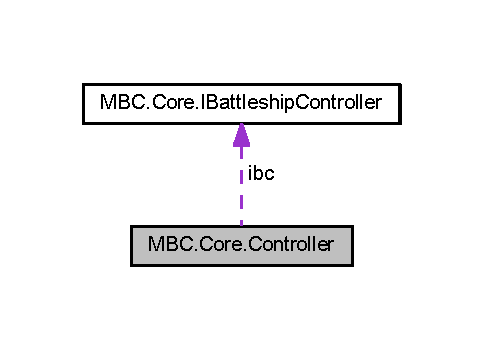
\includegraphics[width=232pt]{class_m_b_c_1_1_core_1_1_controller__coll__graph}
\end{center}
\end{figure}
\subsection*{Public Member Functions}
\begin{DoxyCompactItemize}
\item 
\hyperlink{class_m_b_c_1_1_core_1_1_controller_ada907b30a847119b01f0d52fa6b05633}{Controller} (\hyperlink{interface_m_b_c_1_1_core_1_1_i_battleship_controller}{I\-Battleship\-Controller} ic, \hyperlink{class_m_b_c_1_1_core_1_1_field}{Field} f)
\begin{DoxyCompactList}\small\item\em Sets up this Battleship\-Opponent\end{DoxyCompactList}\item 
\hyperlink{class_m_b_c_1_1_core_1_1_field_1_1_controller_info}{Field.\-Controller\-Info} \hyperlink{class_m_b_c_1_1_core_1_1_controller_af6f8a1a759c38557608ab0faebf49424}{Get\-Field\-Info} ()
\item 
long \hyperlink{class_m_b_c_1_1_core_1_1_controller_afdec43bffe7e30eb0e419c1db641a7f3}{Get\-Time\-Taken} ()
\item 
bool \hyperlink{class_m_b_c_1_1_core_1_1_controller_af4f0b5d25e8b772e7d333d06548d1f4b}{Ships\-Ready} ()
\begin{DoxyCompactList}\small\item\em Checks whether all of the ships have been placed in valid locations\end{DoxyCompactList}\item 
void \hyperlink{class_m_b_c_1_1_core_1_1_controller_a880c9ad7cd60528cad4f36da11bfd9bf}{New\-Match} (string opponent)
\begin{DoxyCompactList}\small\item\em Notifys the player that they are matched up with a new opponent.\end{DoxyCompactList}\item 
bool \hyperlink{class_m_b_c_1_1_core_1_1_controller_a6c4fc9aca31480cdfcbb3d4b1d0fd9e2}{Ran\-Out\-Of\-Time} ()
\begin{DoxyCompactList}\small\item\em Determines if the stopwatch time passed the maximum time allowed.\end{DoxyCompactList}\item 
bool \hyperlink{class_m_b_c_1_1_core_1_1_controller_ae87c31349a7fde4034942a1b505d372d}{New\-Game} ()
\begin{DoxyCompactList}\small\item\em Resets certain data for a new game and notifys the player of the new game being commenced\end{DoxyCompactList}\item 
bool \hyperlink{class_m_b_c_1_1_core_1_1_controller_a5d27318689d6b9e09d6726a433e2b95b}{Place\-Ships} (List$<$ \hyperlink{class_m_b_c_1_1_core_1_1_ship}{Ship} $>$ new\-Ships)
\begin{DoxyCompactList}\small\item\em Notifys the player to make ship placements.\end{DoxyCompactList}\item 
\hyperlink{class_m_b_c_1_1_core_1_1_ship}{Ship} \hyperlink{class_m_b_c_1_1_core_1_1_controller_a21e92036de8a74a82b2d5bc341977359}{Get\-Ship\-At\-Point} (Point p)
\item 
bool \hyperlink{class_m_b_c_1_1_core_1_1_controller_a9e6f3efa65c34223a9753b1c155ef945}{Is\-Alive} (List$<$ Point $>$ shots)
\item 
Point \hyperlink{class_m_b_c_1_1_core_1_1_controller_aee5fa47ba84df60578a2777bd2a77f95}{Shoot\-At} (\hyperlink{class_m_b_c_1_1_core_1_1_controller}{Controller} opponent)
\begin{DoxyCompactList}\small\item\em Asks for the player's shot. Shoot\-At will repeatedly request the shot until it hasn't made the same shot twice.\end{DoxyCompactList}\item 
bool \hyperlink{class_m_b_c_1_1_core_1_1_controller_a5a722dfa61f662d4c6ed9cf1c0f2debc}{Opponent\-Shot} (Point shot)
\begin{DoxyCompactList}\small\item\em Notifys the player that a shot has been made by the other opponent at a certain Point\end{DoxyCompactList}\item 
bool \hyperlink{class_m_b_c_1_1_core_1_1_controller_aa102974b8aeaed8b05a9a9c51793b9d8}{Shot\-Hit} (Point shot, bool sunk)
\begin{DoxyCompactList}\small\item\em Notifys the player that their shot hit a ship at the specified point\end{DoxyCompactList}\item 
bool \hyperlink{class_m_b_c_1_1_core_1_1_controller_a5b6b33ce7d17c2002fe30f89eb22b644}{Shot\-Miss} (Point shot)
\begin{DoxyCompactList}\small\item\em Notifys the player that their shot missed at the specified point\end{DoxyCompactList}\item 
\hypertarget{class_m_b_c_1_1_core_1_1_controller_a48997aafea2900e29f042c71a2131522}{void \hyperlink{class_m_b_c_1_1_core_1_1_controller_a48997aafea2900e29f042c71a2131522}{Game\-Won} ()}\label{class_m_b_c_1_1_core_1_1_controller_a48997aafea2900e29f042c71a2131522}

\begin{DoxyCompactList}\small\item\em Notifys the player that a game has been won, and increments this player's score.\end{DoxyCompactList}\item 
\hypertarget{class_m_b_c_1_1_core_1_1_controller_afe80359151442aaa5c45dc517bd3e8b2}{void \hyperlink{class_m_b_c_1_1_core_1_1_controller_afe80359151442aaa5c45dc517bd3e8b2}{Game\-Lost} ()}\label{class_m_b_c_1_1_core_1_1_controller_afe80359151442aaa5c45dc517bd3e8b2}

\begin{DoxyCompactList}\small\item\em Notifys the player that a game has been lost\end{DoxyCompactList}\item 
\hypertarget{class_m_b_c_1_1_core_1_1_controller_a1beaca8b029cff045923c06b24114653}{void \hyperlink{class_m_b_c_1_1_core_1_1_controller_a1beaca8b029cff045923c06b24114653}{Match\-Over} ()}\label{class_m_b_c_1_1_core_1_1_controller_a1beaca8b029cff045923c06b24114653}

\begin{DoxyCompactList}\small\item\em Notifys the player that a matchup is over\end{DoxyCompactList}\item 
\hypertarget{class_m_b_c_1_1_core_1_1_controller_a75fb8c7721eafa5a0d041d15218fcef6}{override string \hyperlink{class_m_b_c_1_1_core_1_1_controller_a75fb8c7721eafa5a0d041d15218fcef6}{To\-String} ()}\label{class_m_b_c_1_1_core_1_1_controller_a75fb8c7721eafa5a0d041d15218fcef6}

\begin{DoxyCompactList}\small\item\em Generates a string containing the name and version of the encapsulated I\-Battleship\-Opponent\end{DoxyCompactList}\end{DoxyCompactItemize}
\subsection*{Public Attributes}
\begin{DoxyCompactItemize}
\item 
\hypertarget{class_m_b_c_1_1_core_1_1_controller_a65073a7fa3a6f434a7c6b24c3d8ab59a}{const int {\bfseries L\-O\-S\-E\-\_\-\-M\-A\-G\-I\-C\-\_\-\-N\-U\-M\-B\-E\-R} = -\/50}\label{class_m_b_c_1_1_core_1_1_controller_a65073a7fa3a6f434a7c6b24c3d8ab59a}

\item 
\hypertarget{class_m_b_c_1_1_core_1_1_controller_ab56cab183d1d2e91940839b3556a7cf3}{\hyperlink{interface_m_b_c_1_1_core_1_1_i_battleship_controller}{I\-Battleship\-Controller} {\bfseries ibc}}\label{class_m_b_c_1_1_core_1_1_controller_ab56cab183d1d2e91940839b3556a7cf3}

\end{DoxyCompactItemize}


\subsection{Detailed Description}
A Battleship\-Opponent is an object that contains various data pertaining to an I\-Battleship\-Opponent class. Battleship\-Opponent contains various methods to aid in game logic.

\subsection{Constructor \& Destructor Documentation}
\hypertarget{class_m_b_c_1_1_core_1_1_controller_ada907b30a847119b01f0d52fa6b05633}{\index{M\-B\-C\-::\-Core\-::\-Controller@{M\-B\-C\-::\-Core\-::\-Controller}!Controller@{Controller}}
\index{Controller@{Controller}!MBC::Core::Controller@{M\-B\-C\-::\-Core\-::\-Controller}}
\subsubsection[{Controller}]{\setlength{\rightskip}{0pt plus 5cm}M\-B\-C.\-Core.\-Controller.\-Controller (
\begin{DoxyParamCaption}
\item[{{\bf I\-Battleship\-Controller}}]{ic, }
\item[{{\bf Field}}]{f}
\end{DoxyParamCaption}
)}}\label{class_m_b_c_1_1_core_1_1_controller_ada907b30a847119b01f0d52fa6b05633}


Sets up this Battleship\-Opponent


\begin{DoxyParams}{Parameters}
{\em ic} & The object that implements the I\-Battleship\-Opponent interface to play the game.\\
\hline
{\em size} & A reference to the board size in the competition\\
\hline
{\em timeout} & A reference to the maximum alloted time in the competition\\
\hline
\end{DoxyParams}


\subsection{Member Function Documentation}
\hypertarget{class_m_b_c_1_1_core_1_1_controller_af6f8a1a759c38557608ab0faebf49424}{\index{M\-B\-C\-::\-Core\-::\-Controller@{M\-B\-C\-::\-Core\-::\-Controller}!Get\-Field\-Info@{Get\-Field\-Info}}
\index{Get\-Field\-Info@{Get\-Field\-Info}!MBC::Core::Controller@{M\-B\-C\-::\-Core\-::\-Controller}}
\subsubsection[{Get\-Field\-Info}]{\setlength{\rightskip}{0pt plus 5cm}{\bf Field.\-Controller\-Info} M\-B\-C.\-Core.\-Controller.\-Get\-Field\-Info (
\begin{DoxyParamCaption}
{}
\end{DoxyParamCaption}
)}}\label{class_m_b_c_1_1_core_1_1_controller_af6f8a1a759c38557608ab0faebf49424}
\begin{DoxyReturn}{Returns}
The information related to this opponent on the battlefield
\end{DoxyReturn}
\hypertarget{class_m_b_c_1_1_core_1_1_controller_a21e92036de8a74a82b2d5bc341977359}{\index{M\-B\-C\-::\-Core\-::\-Controller@{M\-B\-C\-::\-Core\-::\-Controller}!Get\-Ship\-At\-Point@{Get\-Ship\-At\-Point}}
\index{Get\-Ship\-At\-Point@{Get\-Ship\-At\-Point}!MBC::Core::Controller@{M\-B\-C\-::\-Core\-::\-Controller}}
\subsubsection[{Get\-Ship\-At\-Point}]{\setlength{\rightskip}{0pt plus 5cm}{\bf Ship} M\-B\-C.\-Core.\-Controller.\-Get\-Ship\-At\-Point (
\begin{DoxyParamCaption}
\item[{Point}]{p}
\end{DoxyParamCaption}
)}}\label{class_m_b_c_1_1_core_1_1_controller_a21e92036de8a74a82b2d5bc341977359}
\begin{DoxyReturn}{Returns}
The ship at point p. Null if there is no ship.
\end{DoxyReturn}
\hypertarget{class_m_b_c_1_1_core_1_1_controller_afdec43bffe7e30eb0e419c1db641a7f3}{\index{M\-B\-C\-::\-Core\-::\-Controller@{M\-B\-C\-::\-Core\-::\-Controller}!Get\-Time\-Taken@{Get\-Time\-Taken}}
\index{Get\-Time\-Taken@{Get\-Time\-Taken}!MBC::Core::Controller@{M\-B\-C\-::\-Core\-::\-Controller}}
\subsubsection[{Get\-Time\-Taken}]{\setlength{\rightskip}{0pt plus 5cm}long M\-B\-C.\-Core.\-Controller.\-Get\-Time\-Taken (
\begin{DoxyParamCaption}
{}
\end{DoxyParamCaption}
)}}\label{class_m_b_c_1_1_core_1_1_controller_afdec43bffe7e30eb0e419c1db641a7f3}
\begin{DoxyReturn}{Returns}
The time the last action took for this bot to perform.
\end{DoxyReturn}
\hypertarget{class_m_b_c_1_1_core_1_1_controller_a9e6f3efa65c34223a9753b1c155ef945}{\index{M\-B\-C\-::\-Core\-::\-Controller@{M\-B\-C\-::\-Core\-::\-Controller}!Is\-Alive@{Is\-Alive}}
\index{Is\-Alive@{Is\-Alive}!MBC::Core::Controller@{M\-B\-C\-::\-Core\-::\-Controller}}
\subsubsection[{Is\-Alive}]{\setlength{\rightskip}{0pt plus 5cm}bool M\-B\-C.\-Core.\-Controller.\-Is\-Alive (
\begin{DoxyParamCaption}
\item[{List$<$ Point $>$}]{shots}
\end{DoxyParamCaption}
)}}\label{class_m_b_c_1_1_core_1_1_controller_a9e6f3efa65c34223a9753b1c155ef945}
\begin{DoxyReturn}{Returns}
True if the opponent is still in the match, false if the opponent has lost
\end{DoxyReturn}
\hypertarget{class_m_b_c_1_1_core_1_1_controller_ae87c31349a7fde4034942a1b505d372d}{\index{M\-B\-C\-::\-Core\-::\-Controller@{M\-B\-C\-::\-Core\-::\-Controller}!New\-Game@{New\-Game}}
\index{New\-Game@{New\-Game}!MBC::Core::Controller@{M\-B\-C\-::\-Core\-::\-Controller}}
\subsubsection[{New\-Game}]{\setlength{\rightskip}{0pt plus 5cm}bool M\-B\-C.\-Core.\-Controller.\-New\-Game (
\begin{DoxyParamCaption}
{}
\end{DoxyParamCaption}
)}}\label{class_m_b_c_1_1_core_1_1_controller_ae87c31349a7fde4034942a1b505d372d}


Resets certain data for a new game and notifys the player of the new game being commenced

\begin{DoxyReturn}{Returns}
True if the player ran out of time. False if they didn't
\end{DoxyReturn}
\hypertarget{class_m_b_c_1_1_core_1_1_controller_a880c9ad7cd60528cad4f36da11bfd9bf}{\index{M\-B\-C\-::\-Core\-::\-Controller@{M\-B\-C\-::\-Core\-::\-Controller}!New\-Match@{New\-Match}}
\index{New\-Match@{New\-Match}!MBC::Core::Controller@{M\-B\-C\-::\-Core\-::\-Controller}}
\subsubsection[{New\-Match}]{\setlength{\rightskip}{0pt plus 5cm}void M\-B\-C.\-Core.\-Controller.\-New\-Match (
\begin{DoxyParamCaption}
\item[{string}]{opponent}
\end{DoxyParamCaption}
)}}\label{class_m_b_c_1_1_core_1_1_controller_a880c9ad7cd60528cad4f36da11bfd9bf}


Notifys the player that they are matched up with a new opponent.


\begin{DoxyParams}{Parameters}
{\em opponent} & The name of the opponent as a string\\
\hline
\end{DoxyParams}
\hypertarget{class_m_b_c_1_1_core_1_1_controller_a5a722dfa61f662d4c6ed9cf1c0f2debc}{\index{M\-B\-C\-::\-Core\-::\-Controller@{M\-B\-C\-::\-Core\-::\-Controller}!Opponent\-Shot@{Opponent\-Shot}}
\index{Opponent\-Shot@{Opponent\-Shot}!MBC::Core::Controller@{M\-B\-C\-::\-Core\-::\-Controller}}
\subsubsection[{Opponent\-Shot}]{\setlength{\rightskip}{0pt plus 5cm}bool M\-B\-C.\-Core.\-Controller.\-Opponent\-Shot (
\begin{DoxyParamCaption}
\item[{Point}]{shot}
\end{DoxyParamCaption}
)}}\label{class_m_b_c_1_1_core_1_1_controller_a5a722dfa61f662d4c6ed9cf1c0f2debc}


Notifys the player that a shot has been made by the other opponent at a certain Point


\begin{DoxyParams}{Parameters}
{\em shot} & The point where the other opponent shot\\
\hline
\end{DoxyParams}
\begin{DoxyReturn}{Returns}
True if the player ran out of time. False if they didn't
\end{DoxyReturn}
\hypertarget{class_m_b_c_1_1_core_1_1_controller_a5d27318689d6b9e09d6726a433e2b95b}{\index{M\-B\-C\-::\-Core\-::\-Controller@{M\-B\-C\-::\-Core\-::\-Controller}!Place\-Ships@{Place\-Ships}}
\index{Place\-Ships@{Place\-Ships}!MBC::Core::Controller@{M\-B\-C\-::\-Core\-::\-Controller}}
\subsubsection[{Place\-Ships}]{\setlength{\rightskip}{0pt plus 5cm}bool M\-B\-C.\-Core.\-Controller.\-Place\-Ships (
\begin{DoxyParamCaption}
\item[{List$<$ {\bf Ship} $>$}]{new\-Ships}
\end{DoxyParamCaption}
)}}\label{class_m_b_c_1_1_core_1_1_controller_a5d27318689d6b9e09d6726a433e2b95b}


Notifys the player to make ship placements.


\begin{DoxyParams}{Parameters}
{\em new\-Ships} & A list of ships to place\\
\hline
\end{DoxyParams}
\begin{DoxyReturn}{Returns}
True if the player ran out of time. False if they didn't
\end{DoxyReturn}
\hypertarget{class_m_b_c_1_1_core_1_1_controller_a6c4fc9aca31480cdfcbb3d4b1d0fd9e2}{\index{M\-B\-C\-::\-Core\-::\-Controller@{M\-B\-C\-::\-Core\-::\-Controller}!Ran\-Out\-Of\-Time@{Ran\-Out\-Of\-Time}}
\index{Ran\-Out\-Of\-Time@{Ran\-Out\-Of\-Time}!MBC::Core::Controller@{M\-B\-C\-::\-Core\-::\-Controller}}
\subsubsection[{Ran\-Out\-Of\-Time}]{\setlength{\rightskip}{0pt plus 5cm}bool M\-B\-C.\-Core.\-Controller.\-Ran\-Out\-Of\-Time (
\begin{DoxyParamCaption}
{}
\end{DoxyParamCaption}
)}}\label{class_m_b_c_1_1_core_1_1_controller_a6c4fc9aca31480cdfcbb3d4b1d0fd9e2}


Determines if the stopwatch time passed the maximum time allowed.

\begin{DoxyReturn}{Returns}
True if the player ran out of time. False if they didn't
\end{DoxyReturn}
\hypertarget{class_m_b_c_1_1_core_1_1_controller_af4f0b5d25e8b772e7d333d06548d1f4b}{\index{M\-B\-C\-::\-Core\-::\-Controller@{M\-B\-C\-::\-Core\-::\-Controller}!Ships\-Ready@{Ships\-Ready}}
\index{Ships\-Ready@{Ships\-Ready}!MBC::Core::Controller@{M\-B\-C\-::\-Core\-::\-Controller}}
\subsubsection[{Ships\-Ready}]{\setlength{\rightskip}{0pt plus 5cm}bool M\-B\-C.\-Core.\-Controller.\-Ships\-Ready (
\begin{DoxyParamCaption}
{}
\end{DoxyParamCaption}
)}}\label{class_m_b_c_1_1_core_1_1_controller_af4f0b5d25e8b772e7d333d06548d1f4b}


Checks whether all of the ships have been placed in valid locations

\begin{DoxyReturn}{Returns}
True if all ships are placed, not conflicting each other, and in valid locations. False if otherwise
\end{DoxyReturn}
\hypertarget{class_m_b_c_1_1_core_1_1_controller_aee5fa47ba84df60578a2777bd2a77f95}{\index{M\-B\-C\-::\-Core\-::\-Controller@{M\-B\-C\-::\-Core\-::\-Controller}!Shoot\-At@{Shoot\-At}}
\index{Shoot\-At@{Shoot\-At}!MBC::Core::Controller@{M\-B\-C\-::\-Core\-::\-Controller}}
\subsubsection[{Shoot\-At}]{\setlength{\rightskip}{0pt plus 5cm}Point M\-B\-C.\-Core.\-Controller.\-Shoot\-At (
\begin{DoxyParamCaption}
\item[{{\bf Controller}}]{opponent}
\end{DoxyParamCaption}
)}}\label{class_m_b_c_1_1_core_1_1_controller_aee5fa47ba84df60578a2777bd2a77f95}


Asks for the player's shot. Shoot\-At will repeatedly request the shot until it hasn't made the same shot twice.


\begin{DoxyParams}{Parameters}
{\em opponent} & The Battleship\-Opponent to \char`\"{}shoot at\char`\"{}\\
\hline
\end{DoxyParams}
\begin{DoxyReturn}{Returns}
The point the player has shot at. If the player ran out of time, a point at (L\-O\-S\-E\-\_\-\-M\-A\-G\-I\-C\-\_\-\-N\-U\-M\-B\-E\-R, L\-O\-S\-E\-\_\-\-M\-A\-G\-I\-C\-\_\-\-N\-U\-M\-B\-E\-R) will be returned instead.
\end{DoxyReturn}
\hypertarget{class_m_b_c_1_1_core_1_1_controller_aa102974b8aeaed8b05a9a9c51793b9d8}{\index{M\-B\-C\-::\-Core\-::\-Controller@{M\-B\-C\-::\-Core\-::\-Controller}!Shot\-Hit@{Shot\-Hit}}
\index{Shot\-Hit@{Shot\-Hit}!MBC::Core::Controller@{M\-B\-C\-::\-Core\-::\-Controller}}
\subsubsection[{Shot\-Hit}]{\setlength{\rightskip}{0pt plus 5cm}bool M\-B\-C.\-Core.\-Controller.\-Shot\-Hit (
\begin{DoxyParamCaption}
\item[{Point}]{shot, }
\item[{bool}]{sunk}
\end{DoxyParamCaption}
)}}\label{class_m_b_c_1_1_core_1_1_controller_aa102974b8aeaed8b05a9a9c51793b9d8}


Notifys the player that their shot hit a ship at the specified point


\begin{DoxyParams}{Parameters}
{\em shot} & The point at which the players shot hit a ship\\
\hline
{\em sunk} & If the shot sunk a ship\\
\hline
\end{DoxyParams}
\begin{DoxyReturn}{Returns}
True if the player ran out of time. False if they didn't
\end{DoxyReturn}
\hypertarget{class_m_b_c_1_1_core_1_1_controller_a5b6b33ce7d17c2002fe30f89eb22b644}{\index{M\-B\-C\-::\-Core\-::\-Controller@{M\-B\-C\-::\-Core\-::\-Controller}!Shot\-Miss@{Shot\-Miss}}
\index{Shot\-Miss@{Shot\-Miss}!MBC::Core::Controller@{M\-B\-C\-::\-Core\-::\-Controller}}
\subsubsection[{Shot\-Miss}]{\setlength{\rightskip}{0pt plus 5cm}bool M\-B\-C.\-Core.\-Controller.\-Shot\-Miss (
\begin{DoxyParamCaption}
\item[{Point}]{shot}
\end{DoxyParamCaption}
)}}\label{class_m_b_c_1_1_core_1_1_controller_a5b6b33ce7d17c2002fe30f89eb22b644}


Notifys the player that their shot missed at the specified point


\begin{DoxyParams}{Parameters}
{\em shot} & The point the player shot at but missed\\
\hline
\end{DoxyParams}
\begin{DoxyReturn}{Returns}
True if the player ran out of time. False if they didn't
\end{DoxyReturn}


The documentation for this class was generated from the following file\-:\begin{DoxyCompactItemize}
\item 
M\-B\-C Core/Controller.\-cs\end{DoxyCompactItemize}

\hypertarget{class_m_b_c_1_1_core_1_1_field_1_1_controller_info}{\section{M\-B\-C.\-Core.\-Field.\-Controller\-Info Class Reference}
\label{class_m_b_c_1_1_core_1_1_field_1_1_controller_info}\index{M\-B\-C.\-Core.\-Field.\-Controller\-Info@{M\-B\-C.\-Core.\-Field.\-Controller\-Info}}
}


Contains information related to the state of the battlefield for each opponent. 


\subsection*{Public Member Functions}
\begin{DoxyCompactItemize}
\item 
\hypertarget{class_m_b_c_1_1_core_1_1_field_1_1_controller_info_a86a3a39e847075369e6c08e19fad356c}{{\bfseries Controller\-Info} (string ctrl\-Name, Version ctrl\-Version)}\label{class_m_b_c_1_1_core_1_1_field_1_1_controller_info_a86a3a39e847075369e6c08e19fad356c}

\end{DoxyCompactItemize}
\subsection*{Public Attributes}
\begin{DoxyCompactItemize}
\item 
\hypertarget{class_m_b_c_1_1_core_1_1_field_1_1_controller_info_a0e47d7ccd7030340d6b8cb7691bd3d93}{List$<$ Point $>$ {\bfseries shots\-Made}}\label{class_m_b_c_1_1_core_1_1_field_1_1_controller_info_a0e47d7ccd7030340d6b8cb7691bd3d93}

\item 
\hypertarget{class_m_b_c_1_1_core_1_1_field_1_1_controller_info_a6d69c3ee13b7f5779921afc37582d5e1}{List$<$ \hyperlink{class_m_b_c_1_1_core_1_1_ship}{Ship} $>$ {\bfseries ships}}\label{class_m_b_c_1_1_core_1_1_field_1_1_controller_info_a6d69c3ee13b7f5779921afc37582d5e1}

\item 
\hypertarget{class_m_b_c_1_1_core_1_1_field_1_1_controller_info_a04bdad238fa4cc5793a332019760d69f}{int {\bfseries score} = 0}\label{class_m_b_c_1_1_core_1_1_field_1_1_controller_info_a04bdad238fa4cc5793a332019760d69f}

\item 
\hypertarget{class_m_b_c_1_1_core_1_1_field_1_1_controller_info_a0cfcf1cf1be00aff816e54fae75acdfe}{string {\bfseries name}}\label{class_m_b_c_1_1_core_1_1_field_1_1_controller_info_a0cfcf1cf1be00aff816e54fae75acdfe}

\item 
\hypertarget{class_m_b_c_1_1_core_1_1_field_1_1_controller_info_a68c36e4d0a3344408794caf64f6f7a10}{Version {\bfseries version}}\label{class_m_b_c_1_1_core_1_1_field_1_1_controller_info_a68c36e4d0a3344408794caf64f6f7a10}

\end{DoxyCompactItemize}


\subsection{Detailed Description}
Contains information related to the state of the battlefield for each opponent.

The documentation for this class was generated from the following file\-:\begin{DoxyCompactItemize}
\item 
Core/Field.\-cs\end{DoxyCompactItemize}

\hypertarget{class_m_b_c_1_1_core_1_1mbc_1_1accolades_1_1_domination}{\section{M\-B\-C.\-Core.\-mbc.\-accolades.\-Domination Class Reference}
\label{class_m_b_c_1_1_core_1_1mbc_1_1accolades_1_1_domination}\index{M\-B\-C.\-Core.\-mbc.\-accolades.\-Domination@{M\-B\-C.\-Core.\-mbc.\-accolades.\-Domination}}
}


Inheritance diagram for M\-B\-C.\-Core.\-mbc.\-accolades.\-Domination\-:\nopagebreak
\begin{figure}[H]
\begin{center}
\leavevmode
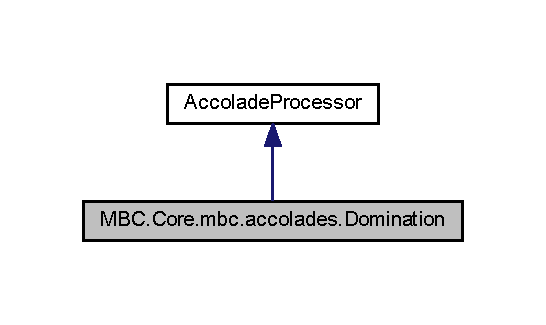
\includegraphics[width=262pt]{class_m_b_c_1_1_core_1_1mbc_1_1accolades_1_1_domination__inherit__graph}
\end{center}
\end{figure}


Collaboration diagram for M\-B\-C.\-Core.\-mbc.\-accolades.\-Domination\-:\nopagebreak
\begin{figure}[H]
\begin{center}
\leavevmode
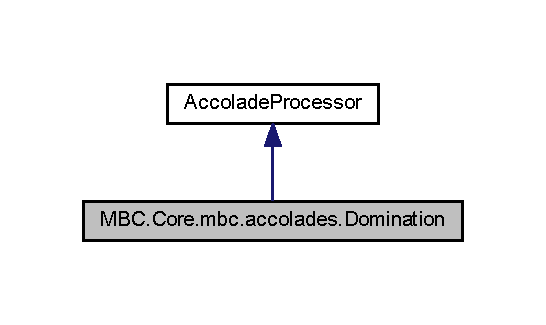
\includegraphics[width=262pt]{class_m_b_c_1_1_core_1_1mbc_1_1accolades_1_1_domination__coll__graph}
\end{center}
\end{figure}
\subsection*{Public Member Functions}
\begin{DoxyCompactItemize}
\item 
\hypertarget{class_m_b_c_1_1_core_1_1mbc_1_1accolades_1_1_domination_a807e3fc62f6f57ba91670cc36ba9bab7}{Round\-Log.\-Round\-Accolade \hyperlink{class_m_b_c_1_1_core_1_1mbc_1_1accolades_1_1_domination_a807e3fc62f6f57ba91670cc36ba9bab7}{Process} (\hyperlink{class_m_b_c_1_1_core_1_1_round_log_1_1_round_activity}{Round\-Log.\-Round\-Activity} a)}\label{class_m_b_c_1_1_core_1_1mbc_1_1accolades_1_1_domination_a807e3fc62f6f57ba91670cc36ba9bab7}

\begin{DoxyCompactList}\small\item\em Process an activity\end{DoxyCompactList}\end{DoxyCompactItemize}


The documentation for this class was generated from the following file\-:\begin{DoxyCompactItemize}
\item 
M\-B\-C Core/accolades/Domination.\-cs\end{DoxyCompactItemize}

\hypertarget{class_m_b_c_1_1_core_1_1mbc_1_1accolades_1_1_fast}{\section{M\-B\-C.\-Core.\-mbc.\-accolades.\-Fast Class Reference}
\label{class_m_b_c_1_1_core_1_1mbc_1_1accolades_1_1_fast}\index{M\-B\-C.\-Core.\-mbc.\-accolades.\-Fast@{M\-B\-C.\-Core.\-mbc.\-accolades.\-Fast}}
}


Inheritance diagram for M\-B\-C.\-Core.\-mbc.\-accolades.\-Fast\-:\nopagebreak
\begin{figure}[H]
\begin{center}
\leavevmode
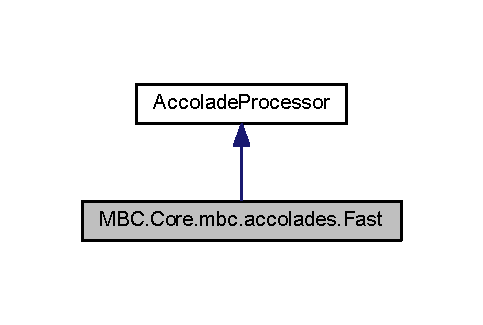
\includegraphics[width=232pt]{class_m_b_c_1_1_core_1_1mbc_1_1accolades_1_1_fast__inherit__graph}
\end{center}
\end{figure}


Collaboration diagram for M\-B\-C.\-Core.\-mbc.\-accolades.\-Fast\-:\nopagebreak
\begin{figure}[H]
\begin{center}
\leavevmode
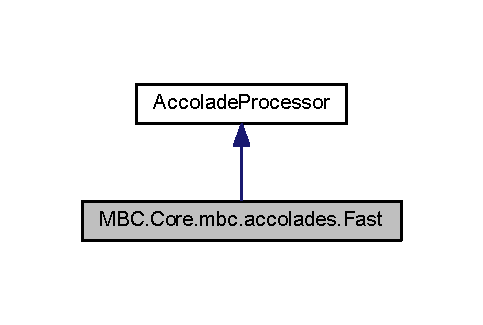
\includegraphics[width=232pt]{class_m_b_c_1_1_core_1_1mbc_1_1accolades_1_1_fast__coll__graph}
\end{center}
\end{figure}
\subsection*{Public Member Functions}
\begin{DoxyCompactItemize}
\item 
\hypertarget{class_m_b_c_1_1_core_1_1mbc_1_1accolades_1_1_fast_a83a0e38fc5d4ddcf5f6c57e7c3baa989}{Round\-Log.\-Round\-Accolade \hyperlink{class_m_b_c_1_1_core_1_1mbc_1_1accolades_1_1_fast_a83a0e38fc5d4ddcf5f6c57e7c3baa989}{Process} (\hyperlink{class_m_b_c_1_1_core_1_1_round_log_1_1_round_activity}{Round\-Log.\-Round\-Activity} a)}\label{class_m_b_c_1_1_core_1_1mbc_1_1accolades_1_1_fast_a83a0e38fc5d4ddcf5f6c57e7c3baa989}

\begin{DoxyCompactList}\small\item\em Process an activity\end{DoxyCompactList}\end{DoxyCompactItemize}


The documentation for this class was generated from the following file\-:\begin{DoxyCompactItemize}
\item 
M\-B\-C Core/accolades/Fast.\-cs\end{DoxyCompactItemize}

\hypertarget{class_m_b_c_1_1_core_1_1_field}{\section{M\-B\-C.\-Core.\-Field Class Reference}
\label{class_m_b_c_1_1_core_1_1_field}\index{M\-B\-C.\-Core.\-Field@{M\-B\-C.\-Core.\-Field}}
}
\subsection*{Classes}
\begin{DoxyCompactItemize}
\item 
class \hyperlink{class_m_b_c_1_1_core_1_1_field_1_1_controller_info}{Controller\-Info}
\begin{DoxyCompactList}\small\item\em Contains information related to the state of the battlefield for each opponent\end{DoxyCompactList}\end{DoxyCompactItemize}
\subsection*{Public Member Functions}
\begin{DoxyCompactItemize}
\item 
\hypertarget{class_m_b_c_1_1_core_1_1_field_a7310ab93b09a8cd557e4fdcc3f686a78}{\hyperlink{class_m_b_c_1_1_core_1_1_field_a7310ab93b09a8cd557e4fdcc3f686a78}{Field} (\hyperlink{interface_m_b_c_1_1_core_1_1_i_battleship_controller}{I\-Battleship\-Controller}\mbox{[}$\,$\mbox{]} ibc)}\label{class_m_b_c_1_1_core_1_1_field_a7310ab93b09a8cd557e4fdcc3f686a78}

\begin{DoxyCompactList}\small\item\em Constructs a Battlefield object initialized with two opponents\end{DoxyCompactList}\item 
\hyperlink{class_m_b_c_1_1_core_1_1_field_1_1_controller_info}{Controller\-Info}\mbox{[}$\,$\mbox{]} \hyperlink{class_m_b_c_1_1_core_1_1_field_aaf565a96cdff422ffed99cccb64b400a}{Get\-Info} ()
\item 
\hypertarget{class_m_b_c_1_1_core_1_1_field_ae135717a6b4f17d3af926751f687b374}{\hyperlink{interface_m_b_c_1_1_core_1_1_i_battleship_controller}{I\-Battleship\-Controller} \hyperlink{class_m_b_c_1_1_core_1_1_field_ae135717a6b4f17d3af926751f687b374}{Get\-Opponent} (\hyperlink{interface_m_b_c_1_1_core_1_1_i_battleship_controller}{I\-Battleship\-Controller} c)}\label{class_m_b_c_1_1_core_1_1_field_ae135717a6b4f17d3af926751f687b374}

\begin{DoxyCompactList}\small\item\em Gets the first occurrence of \hyperlink{interface_m_b_c_1_1_core_1_1_i_battleship_controller}{I\-Battleship\-Controller} that is not equal to c. If used properly, this is the opposing controller to the one specified.\end{DoxyCompactList}\item 
\hypertarget{class_m_b_c_1_1_core_1_1_field_a48bb106fc9697c3a8bd7139d06f4aa09}{\hyperlink{class_m_b_c_1_1_core_1_1_field_a48bb106fc9697c3a8bd7139d06f4aa09}{Field} (\hyperlink{class_m_b_c_1_1_core_1_1_field}{Field} copy)}\label{class_m_b_c_1_1_core_1_1_field_a48bb106fc9697c3a8bd7139d06f4aa09}

\begin{DoxyCompactList}\small\item\em Copy constructor\end{DoxyCompactList}\end{DoxyCompactItemize}
\subsection*{Public Attributes}
\begin{DoxyCompactItemize}
\item 
\hypertarget{class_m_b_c_1_1_core_1_1_field_a3f88e9794a93bdb7f6c2d183404a5b14}{Size {\bfseries game\-Size}}\label{class_m_b_c_1_1_core_1_1_field_a3f88e9794a93bdb7f6c2d183404a5b14}

\item 
\hypertarget{class_m_b_c_1_1_core_1_1_field_a5ec9e449c21321bb1a199efde363fd90}{Random {\bfseries fixed\-Random}}\label{class_m_b_c_1_1_core_1_1_field_a5ec9e449c21321bb1a199efde363fd90}

\item 
\hypertarget{class_m_b_c_1_1_core_1_1_field_a91be7145eb9671b8fe11efdff1292007}{List$<$ int $>$ {\bfseries ship\-Sizes}}\label{class_m_b_c_1_1_core_1_1_field_a91be7145eb9671b8fe11efdff1292007}

\item 
\hypertarget{class_m_b_c_1_1_core_1_1_field_a52843b12dc28e5f52d9a9eb6b8df3eb6}{Time\-Span {\bfseries timeout\-Limit}}\label{class_m_b_c_1_1_core_1_1_field_a52843b12dc28e5f52d9a9eb6b8df3eb6}

\end{DoxyCompactItemize}
\subsection*{Properties}
\begin{DoxyCompactItemize}
\item 
\hyperlink{class_m_b_c_1_1_core_1_1_field_1_1_controller_info}{Controller\-Info} \hyperlink{class_m_b_c_1_1_core_1_1_field_a68bea4ce761a6ddca725e952213a9949}{this\mbox{[}\-I\-Battleship\-Controller i\mbox{]}}\hspace{0.3cm}{\ttfamily  \mbox{[}get\mbox{]}}
\end{DoxyCompactItemize}


\subsection{Member Function Documentation}
\hypertarget{class_m_b_c_1_1_core_1_1_field_aaf565a96cdff422ffed99cccb64b400a}{\index{M\-B\-C\-::\-Core\-::\-Field@{M\-B\-C\-::\-Core\-::\-Field}!Get\-Info@{Get\-Info}}
\index{Get\-Info@{Get\-Info}!MBC::Core::Field@{M\-B\-C\-::\-Core\-::\-Field}}
\subsubsection[{Get\-Info}]{\setlength{\rightskip}{0pt plus 5cm}{\bf Controller\-Info} \mbox{[}$\,$\mbox{]} M\-B\-C.\-Core.\-Field.\-Get\-Info (
\begin{DoxyParamCaption}
{}
\end{DoxyParamCaption}
)}}\label{class_m_b_c_1_1_core_1_1_field_aaf565a96cdff422ffed99cccb64b400a}
\begin{DoxyReturn}{Returns}
Opponent information for both opponents
\end{DoxyReturn}


\subsection{Property Documentation}
\hypertarget{class_m_b_c_1_1_core_1_1_field_a68bea4ce761a6ddca725e952213a9949}{\index{M\-B\-C\-::\-Core\-::\-Field@{M\-B\-C\-::\-Core\-::\-Field}!this\mbox{[}\-I\-Battleship\-Controller i\mbox{]}@{this[I\-Battleship\-Controller i]}}
\index{this\mbox{[}\-I\-Battleship\-Controller i\mbox{]}@{this[I\-Battleship\-Controller i]}!MBC::Core::Field@{M\-B\-C\-::\-Core\-::\-Field}}
\subsubsection[{this[I\-Battleship\-Controller i]}]{\setlength{\rightskip}{0pt plus 5cm}{\bf Controller\-Info} M\-B\-C.\-Core.\-Field.\-this\mbox{[}{\bf I\-Battleship\-Controller} i\mbox{]}\hspace{0.3cm}{\ttfamily [get]}}}\label{class_m_b_c_1_1_core_1_1_field_a68bea4ce761a6ddca725e952213a9949}
\begin{DoxyReturn}{Returns}
The opponent information for the field from the opponent
\end{DoxyReturn}


The documentation for this class was generated from the following file\-:\begin{DoxyCompactItemize}
\item 
Core/Field.\-cs\end{DoxyCompactItemize}

\hypertarget{class_m_b_c_1_1_w_p_f_1_1_field}{\section{M\-B\-C.\-W\-P\-F.\-Field Class Reference}
\label{class_m_b_c_1_1_w_p_f_1_1_field}\index{M\-B\-C.\-W\-P\-F.\-Field@{M\-B\-C.\-W\-P\-F.\-Field}}
}


Interaction logic for Field.\-xaml  




Inheritance diagram for M\-B\-C.\-W\-P\-F.\-Field\-:
\nopagebreak
\begin{figure}[H]
\begin{center}
\leavevmode
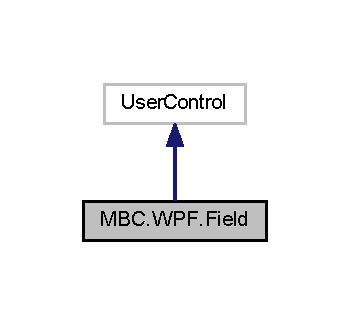
\includegraphics[width=168pt]{class_m_b_c_1_1_w_p_f_1_1_field__inherit__graph}
\end{center}
\end{figure}


Collaboration diagram for M\-B\-C.\-W\-P\-F.\-Field\-:
\nopagebreak
\begin{figure}[H]
\begin{center}
\leavevmode
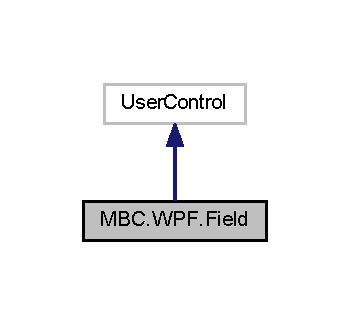
\includegraphics[width=168pt]{class_m_b_c_1_1_w_p_f_1_1_field__coll__graph}
\end{center}
\end{figure}


\subsection{Detailed Description}
Interaction logic for Field.\-xaml 



The documentation for this class was generated from the following file\-:\begin{DoxyCompactItemize}
\item 
M\-B\-C W\-P\-F/Field.\-xaml.\-cs\end{DoxyCompactItemize}

\hypertarget{class_xaml_generated_namespace_1_1_generated_internal_type_helper}{\section{Xaml\-Generated\-Namespace.\-Generated\-Internal\-Type\-Helper Class Reference}
\label{class_xaml_generated_namespace_1_1_generated_internal_type_helper}\index{Xaml\-Generated\-Namespace.\-Generated\-Internal\-Type\-Helper@{Xaml\-Generated\-Namespace.\-Generated\-Internal\-Type\-Helper}}
}


\hyperlink{class_xaml_generated_namespace_1_1_generated_internal_type_helper}{Generated\-Internal\-Type\-Helper}  




Inheritance diagram for Xaml\-Generated\-Namespace.\-Generated\-Internal\-Type\-Helper\-:\nopagebreak
\begin{figure}[H]
\begin{center}
\leavevmode
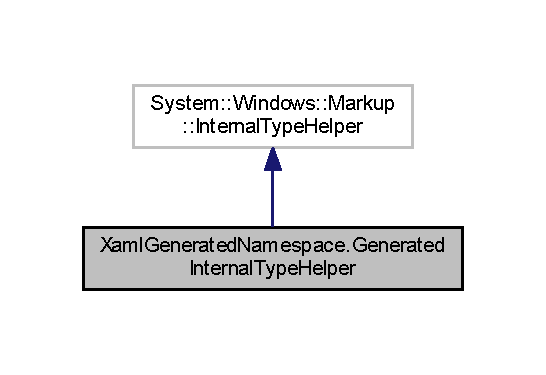
\includegraphics[width=262pt]{class_xaml_generated_namespace_1_1_generated_internal_type_helper__inherit__graph}
\end{center}
\end{figure}


Collaboration diagram for Xaml\-Generated\-Namespace.\-Generated\-Internal\-Type\-Helper\-:\nopagebreak
\begin{figure}[H]
\begin{center}
\leavevmode
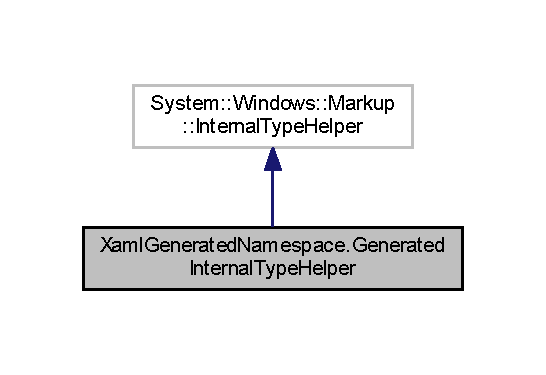
\includegraphics[width=262pt]{class_xaml_generated_namespace_1_1_generated_internal_type_helper__coll__graph}
\end{center}
\end{figure}
\subsection*{Protected Member Functions}
\begin{DoxyCompactItemize}
\item 
override object \hyperlink{class_xaml_generated_namespace_1_1_generated_internal_type_helper_aefb7a98fceb9c287cef4756942f441d1}{Create\-Instance} (System.\-Type type, System.\-Globalization.\-Culture\-Info culture)
\begin{DoxyCompactList}\small\item\em Create\-Instance \end{DoxyCompactList}\item 
override object \hyperlink{class_xaml_generated_namespace_1_1_generated_internal_type_helper_afdc9fe15b56607d02082908d934480c6}{Get\-Property\-Value} (System.\-Reflection.\-Property\-Info property\-Info, object target, System.\-Globalization.\-Culture\-Info culture)
\begin{DoxyCompactList}\small\item\em Get\-Property\-Value \end{DoxyCompactList}\item 
override void \hyperlink{class_xaml_generated_namespace_1_1_generated_internal_type_helper_ade0f04c0f7b18dd5b170e071d5534d38}{Set\-Property\-Value} (System.\-Reflection.\-Property\-Info property\-Info, object target, object value, System.\-Globalization.\-Culture\-Info culture)
\begin{DoxyCompactList}\small\item\em Set\-Property\-Value \end{DoxyCompactList}\item 
override System.\-Delegate \hyperlink{class_xaml_generated_namespace_1_1_generated_internal_type_helper_a8ec4c37e82d9f4e867e9655f4eac3a78}{Create\-Delegate} (System.\-Type delegate\-Type, object target, string handler)
\begin{DoxyCompactList}\small\item\em Create\-Delegate \end{DoxyCompactList}\item 
override void \hyperlink{class_xaml_generated_namespace_1_1_generated_internal_type_helper_a73471f4a6d1ca4c4fceec9ad8610f0c8}{Add\-Event\-Handler} (System.\-Reflection.\-Event\-Info event\-Info, object target, System.\-Delegate handler)
\begin{DoxyCompactList}\small\item\em Add\-Event\-Handler \end{DoxyCompactList}\end{DoxyCompactItemize}


\subsection{Detailed Description}
\hyperlink{class_xaml_generated_namespace_1_1_generated_internal_type_helper}{Generated\-Internal\-Type\-Helper} 



\subsection{Member Function Documentation}
\hypertarget{class_xaml_generated_namespace_1_1_generated_internal_type_helper_a73471f4a6d1ca4c4fceec9ad8610f0c8}{\index{Xaml\-Generated\-Namespace\-::\-Generated\-Internal\-Type\-Helper@{Xaml\-Generated\-Namespace\-::\-Generated\-Internal\-Type\-Helper}!Add\-Event\-Handler@{Add\-Event\-Handler}}
\index{Add\-Event\-Handler@{Add\-Event\-Handler}!XamlGeneratedNamespace::GeneratedInternalTypeHelper@{Xaml\-Generated\-Namespace\-::\-Generated\-Internal\-Type\-Helper}}
\subsubsection[{Add\-Event\-Handler}]{\setlength{\rightskip}{0pt plus 5cm}override void Xaml\-Generated\-Namespace.\-Generated\-Internal\-Type\-Helper.\-Add\-Event\-Handler (
\begin{DoxyParamCaption}
\item[{System.\-Reflection.\-Event\-Info}]{event\-Info, }
\item[{object}]{target, }
\item[{System.\-Delegate}]{handler}
\end{DoxyParamCaption}
)\hspace{0.3cm}{\ttfamily [protected]}}}\label{class_xaml_generated_namespace_1_1_generated_internal_type_helper_a73471f4a6d1ca4c4fceec9ad8610f0c8}


Add\-Event\-Handler 

\hypertarget{class_xaml_generated_namespace_1_1_generated_internal_type_helper_a8ec4c37e82d9f4e867e9655f4eac3a78}{\index{Xaml\-Generated\-Namespace\-::\-Generated\-Internal\-Type\-Helper@{Xaml\-Generated\-Namespace\-::\-Generated\-Internal\-Type\-Helper}!Create\-Delegate@{Create\-Delegate}}
\index{Create\-Delegate@{Create\-Delegate}!XamlGeneratedNamespace::GeneratedInternalTypeHelper@{Xaml\-Generated\-Namespace\-::\-Generated\-Internal\-Type\-Helper}}
\subsubsection[{Create\-Delegate}]{\setlength{\rightskip}{0pt plus 5cm}override System.\-Delegate Xaml\-Generated\-Namespace.\-Generated\-Internal\-Type\-Helper.\-Create\-Delegate (
\begin{DoxyParamCaption}
\item[{System.\-Type}]{delegate\-Type, }
\item[{object}]{target, }
\item[{string}]{handler}
\end{DoxyParamCaption}
)\hspace{0.3cm}{\ttfamily [protected]}}}\label{class_xaml_generated_namespace_1_1_generated_internal_type_helper_a8ec4c37e82d9f4e867e9655f4eac3a78}


Create\-Delegate 

\hypertarget{class_xaml_generated_namespace_1_1_generated_internal_type_helper_aefb7a98fceb9c287cef4756942f441d1}{\index{Xaml\-Generated\-Namespace\-::\-Generated\-Internal\-Type\-Helper@{Xaml\-Generated\-Namespace\-::\-Generated\-Internal\-Type\-Helper}!Create\-Instance@{Create\-Instance}}
\index{Create\-Instance@{Create\-Instance}!XamlGeneratedNamespace::GeneratedInternalTypeHelper@{Xaml\-Generated\-Namespace\-::\-Generated\-Internal\-Type\-Helper}}
\subsubsection[{Create\-Instance}]{\setlength{\rightskip}{0pt plus 5cm}override object Xaml\-Generated\-Namespace.\-Generated\-Internal\-Type\-Helper.\-Create\-Instance (
\begin{DoxyParamCaption}
\item[{System.\-Type}]{type, }
\item[{System.\-Globalization.\-Culture\-Info}]{culture}
\end{DoxyParamCaption}
)\hspace{0.3cm}{\ttfamily [protected]}}}\label{class_xaml_generated_namespace_1_1_generated_internal_type_helper_aefb7a98fceb9c287cef4756942f441d1}


Create\-Instance 

\hypertarget{class_xaml_generated_namespace_1_1_generated_internal_type_helper_afdc9fe15b56607d02082908d934480c6}{\index{Xaml\-Generated\-Namespace\-::\-Generated\-Internal\-Type\-Helper@{Xaml\-Generated\-Namespace\-::\-Generated\-Internal\-Type\-Helper}!Get\-Property\-Value@{Get\-Property\-Value}}
\index{Get\-Property\-Value@{Get\-Property\-Value}!XamlGeneratedNamespace::GeneratedInternalTypeHelper@{Xaml\-Generated\-Namespace\-::\-Generated\-Internal\-Type\-Helper}}
\subsubsection[{Get\-Property\-Value}]{\setlength{\rightskip}{0pt plus 5cm}override object Xaml\-Generated\-Namespace.\-Generated\-Internal\-Type\-Helper.\-Get\-Property\-Value (
\begin{DoxyParamCaption}
\item[{System.\-Reflection.\-Property\-Info}]{property\-Info, }
\item[{object}]{target, }
\item[{System.\-Globalization.\-Culture\-Info}]{culture}
\end{DoxyParamCaption}
)\hspace{0.3cm}{\ttfamily [protected]}}}\label{class_xaml_generated_namespace_1_1_generated_internal_type_helper_afdc9fe15b56607d02082908d934480c6}


Get\-Property\-Value 

\hypertarget{class_xaml_generated_namespace_1_1_generated_internal_type_helper_ade0f04c0f7b18dd5b170e071d5534d38}{\index{Xaml\-Generated\-Namespace\-::\-Generated\-Internal\-Type\-Helper@{Xaml\-Generated\-Namespace\-::\-Generated\-Internal\-Type\-Helper}!Set\-Property\-Value@{Set\-Property\-Value}}
\index{Set\-Property\-Value@{Set\-Property\-Value}!XamlGeneratedNamespace::GeneratedInternalTypeHelper@{Xaml\-Generated\-Namespace\-::\-Generated\-Internal\-Type\-Helper}}
\subsubsection[{Set\-Property\-Value}]{\setlength{\rightskip}{0pt plus 5cm}override void Xaml\-Generated\-Namespace.\-Generated\-Internal\-Type\-Helper.\-Set\-Property\-Value (
\begin{DoxyParamCaption}
\item[{System.\-Reflection.\-Property\-Info}]{property\-Info, }
\item[{object}]{target, }
\item[{object}]{value, }
\item[{System.\-Globalization.\-Culture\-Info}]{culture}
\end{DoxyParamCaption}
)\hspace{0.3cm}{\ttfamily [protected]}}}\label{class_xaml_generated_namespace_1_1_generated_internal_type_helper_ade0f04c0f7b18dd5b170e071d5534d38}


Set\-Property\-Value 



The documentation for this class was generated from the following file\-:\begin{DoxyCompactItemize}
\item 
App\-W\-P\-F/obj/x86/\-Debug/Generated\-Internal\-Type\-Helper.\-g.\-i.\-cs\end{DoxyCompactItemize}

\hypertarget{class_m_b_c_1_1_core_1_1mbc_1_1accolades_1_1_head_to_head}{\section{M\-B\-C.\-Core.\-mbc.\-accolades.\-Head\-To\-Head Class Reference}
\label{class_m_b_c_1_1_core_1_1mbc_1_1accolades_1_1_head_to_head}\index{M\-B\-C.\-Core.\-mbc.\-accolades.\-Head\-To\-Head@{M\-B\-C.\-Core.\-mbc.\-accolades.\-Head\-To\-Head}}
}


Inheritance diagram for M\-B\-C.\-Core.\-mbc.\-accolades.\-Head\-To\-Head\-:\nopagebreak
\begin{figure}[H]
\begin{center}
\leavevmode
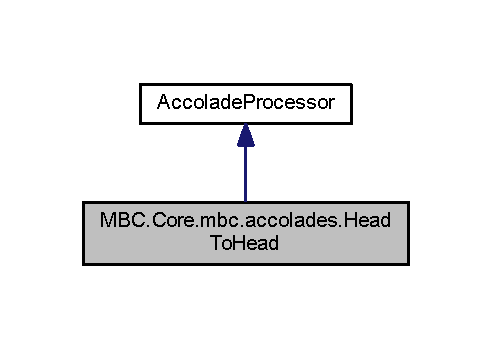
\includegraphics[width=236pt]{class_m_b_c_1_1_core_1_1mbc_1_1accolades_1_1_head_to_head__inherit__graph}
\end{center}
\end{figure}


Collaboration diagram for M\-B\-C.\-Core.\-mbc.\-accolades.\-Head\-To\-Head\-:\nopagebreak
\begin{figure}[H]
\begin{center}
\leavevmode
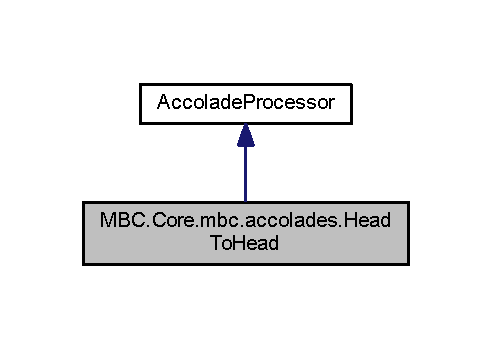
\includegraphics[width=236pt]{class_m_b_c_1_1_core_1_1mbc_1_1accolades_1_1_head_to_head__coll__graph}
\end{center}
\end{figure}
\subsection*{Public Member Functions}
\begin{DoxyCompactItemize}
\item 
\hypertarget{class_m_b_c_1_1_core_1_1mbc_1_1accolades_1_1_head_to_head_abd8eabe255b8b53e059d4ac2a3f85598}{Round\-Log.\-Round\-Accolade \hyperlink{class_m_b_c_1_1_core_1_1mbc_1_1accolades_1_1_head_to_head_abd8eabe255b8b53e059d4ac2a3f85598}{Process} (\hyperlink{class_m_b_c_1_1_core_1_1_round_log_1_1_round_activity}{Round\-Log.\-Round\-Activity} a)}\label{class_m_b_c_1_1_core_1_1mbc_1_1accolades_1_1_head_to_head_abd8eabe255b8b53e059d4ac2a3f85598}

\begin{DoxyCompactList}\small\item\em Process an activity\end{DoxyCompactList}\end{DoxyCompactItemize}


The documentation for this class was generated from the following file\-:\begin{DoxyCompactItemize}
\item 
M\-B\-C Core/accolades/Head\-To\-Head.\-cs\end{DoxyCompactItemize}

\hypertarget{interface_m_b_c_1_1_core_1_1_i_battleship_controller}{\section{M\-B\-C.\-Core.\-I\-Battleship\-Controller Interface Reference}
\label{interface_m_b_c_1_1_core_1_1_i_battleship_controller}\index{M\-B\-C.\-Core.\-I\-Battleship\-Controller@{M\-B\-C.\-Core.\-I\-Battleship\-Controller}}
}


This interface is to be implemented by any class that is to participate in a battleship competition.  




Inheritance diagram for M\-B\-C.\-Core.\-I\-Battleship\-Controller\-:
\nopagebreak
\begin{figure}[H]
\begin{center}
\leavevmode
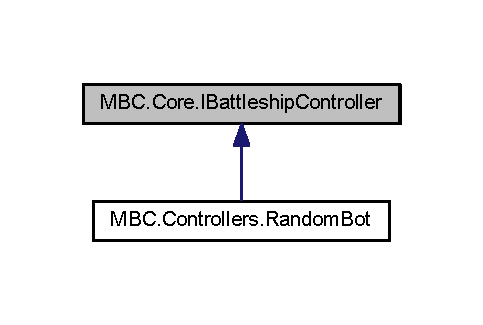
\includegraphics[width=232pt]{interface_m_b_c_1_1_core_1_1_i_battleship_controller__inherit__graph}
\end{center}
\end{figure}
\subsection*{Public Member Functions}
\begin{DoxyCompactItemize}
\item 
void \hyperlink{interface_m_b_c_1_1_core_1_1_i_battleship_controller_a44c7a001b2005e411ccb894223efa3d9}{New\-Match} (string opponent)
\begin{DoxyCompactList}\small\item\em Called when this \hyperlink{interface_m_b_c_1_1_core_1_1_i_battleship_controller}{I\-Battleship\-Controller} has been matched up with another \hyperlink{interface_m_b_c_1_1_core_1_1_i_battleship_controller}{I\-Battleship\-Controller} on the field.\end{DoxyCompactList}\item 
void \hyperlink{interface_m_b_c_1_1_core_1_1_i_battleship_controller_a17dafb26838363ab7630278962523828}{New\-Game} (Size size, Time\-Span time\-Span, Random rand)
\begin{DoxyCompactList}\small\item\em Called when a new game (round) is commencing.\end{DoxyCompactList}\item 
void \hyperlink{interface_m_b_c_1_1_core_1_1_i_battleship_controller_aacd76e5a0143ed65b3cd4f911b658866}{Place\-Ships} (Read\-Only\-Collection$<$ \hyperlink{class_m_b_c_1_1_core_1_1_ship}{Ship} $>$ ships)
\begin{DoxyCompactList}\small\item\em Called when this I\-Battleship\-Opponent must place their ships. Utilize the \hyperlink{class_m_b_c_1_1_core_1_1_ship}{Ship} objects in the given collection to place ships. Do not provide invalid ship placements (overlapping, bad coords, etc.)\end{DoxyCompactList}\item 
Point \hyperlink{interface_m_b_c_1_1_core_1_1_i_battleship_controller_a1e3990b3561cdc6980332b60359d797a}{Get\-Shot} ()
\begin{DoxyCompactList}\small\item\em Called when this I\-Battleship\-Opponent has the opportunity to make a shot in their turn.\end{DoxyCompactList}\item 
void \hyperlink{interface_m_b_c_1_1_core_1_1_i_battleship_controller_ae8805f1f06e67901db8be2665076582f}{Opponent\-Shot} (Point shot)
\begin{DoxyCompactList}\small\item\em Called when this I\-Battleship\-Opponent is being shot at by the opponent.\end{DoxyCompactList}\item 
void \hyperlink{interface_m_b_c_1_1_core_1_1_i_battleship_controller_a4082a60bb8f9873c9ac794953da6563b}{Shot\-Hit} (Point shot, bool sunk)
\begin{DoxyCompactList}\small\item\em Called when this I\-Battleship\-Opponent has hit an opponent ship from the Point given by a previous call to \hyperlink{interface_m_b_c_1_1_core_1_1_i_battleship_controller_a1e3990b3561cdc6980332b60359d797a}{Get\-Shot()}.\end{DoxyCompactList}\item 
void \hyperlink{interface_m_b_c_1_1_core_1_1_i_battleship_controller_ac0806bdf4ceb486920d78c19a088b507}{Shot\-Miss} (Point shot)
\begin{DoxyCompactList}\small\item\em Called when this I\-Battleship\-Opponent did not hit an opponent ship from the Point given by a previous call to \hyperlink{interface_m_b_c_1_1_core_1_1_i_battleship_controller_a1e3990b3561cdc6980332b60359d797a}{Get\-Shot()}.\end{DoxyCompactList}\item 
\hypertarget{interface_m_b_c_1_1_core_1_1_i_battleship_controller_add0a1ee69c8b1ee623635a6886263841}{void \hyperlink{interface_m_b_c_1_1_core_1_1_i_battleship_controller_add0a1ee69c8b1ee623635a6886263841}{Game\-Won} ()}\label{interface_m_b_c_1_1_core_1_1_i_battleship_controller_add0a1ee69c8b1ee623635a6886263841}

\begin{DoxyCompactList}\small\item\em Called when a game (round) is over. In this case, this \hyperlink{interface_m_b_c_1_1_core_1_1_i_battleship_controller}{I\-Battleship\-Controller} has won the round.\end{DoxyCompactList}\item 
\hypertarget{interface_m_b_c_1_1_core_1_1_i_battleship_controller_a0d0534e190e468cdfb1d7a333dc025d7}{void \hyperlink{interface_m_b_c_1_1_core_1_1_i_battleship_controller_a0d0534e190e468cdfb1d7a333dc025d7}{Game\-Lost} ()}\label{interface_m_b_c_1_1_core_1_1_i_battleship_controller_a0d0534e190e468cdfb1d7a333dc025d7}

\begin{DoxyCompactList}\small\item\em Called when a game (round) is over. In this case, this I\-Battelship\-Controller has lost the round.\end{DoxyCompactList}\item 
\hypertarget{interface_m_b_c_1_1_core_1_1_i_battleship_controller_a35963db7e91bf53b2f9152898659e098}{void \hyperlink{interface_m_b_c_1_1_core_1_1_i_battleship_controller_a35963db7e91bf53b2f9152898659e098}{Match\-Over} ()}\label{interface_m_b_c_1_1_core_1_1_i_battleship_controller_a35963db7e91bf53b2f9152898659e098}

\begin{DoxyCompactList}\small\item\em Called when a competition matchup is over. Note that a matchup can start up again with the same parameters.\end{DoxyCompactList}\end{DoxyCompactItemize}
\subsection*{Properties}
\begin{DoxyCompactItemize}
\item 
\hypertarget{interface_m_b_c_1_1_core_1_1_i_battleship_controller_a6a6130592110828d325bc93e1d55586d}{string \hyperlink{interface_m_b_c_1_1_core_1_1_i_battleship_controller_a6a6130592110828d325bc93e1d55586d}{Name}\hspace{0.3cm}{\ttfamily  \mbox{[}get\mbox{]}}}\label{interface_m_b_c_1_1_core_1_1_i_battleship_controller_a6a6130592110828d325bc93e1d55586d}

\begin{DoxyCompactList}\small\item\em Gets a string that represents the name of this \hyperlink{interface_m_b_c_1_1_core_1_1_i_battleship_controller}{I\-Battleship\-Controller}.\end{DoxyCompactList}\item 
\hypertarget{interface_m_b_c_1_1_core_1_1_i_battleship_controller_a526e01cd2a35e521f0965b3fbb1b4cd4}{Version \hyperlink{interface_m_b_c_1_1_core_1_1_i_battleship_controller_a526e01cd2a35e521f0965b3fbb1b4cd4}{Version}\hspace{0.3cm}{\ttfamily  \mbox{[}get\mbox{]}}}\label{interface_m_b_c_1_1_core_1_1_i_battleship_controller_a526e01cd2a35e521f0965b3fbb1b4cd4}

\begin{DoxyCompactList}\small\item\em Gets a Version object that represents the assembly version of this \hyperlink{interface_m_b_c_1_1_core_1_1_i_battleship_controller}{I\-Battleship\-Controller}.\end{DoxyCompactList}\end{DoxyCompactItemize}


\subsection{Detailed Description}
This interface is to be implemented by any class that is to participate in a battleship competition. 

The various methods in this class are called at times during the battleship competition. Read over the documentation for each method to understand when these methods are invoked. 

\subsection{Member Function Documentation}
\hypertarget{interface_m_b_c_1_1_core_1_1_i_battleship_controller_a1e3990b3561cdc6980332b60359d797a}{\index{M\-B\-C\-::\-Core\-::\-I\-Battleship\-Controller@{M\-B\-C\-::\-Core\-::\-I\-Battleship\-Controller}!Get\-Shot@{Get\-Shot}}
\index{Get\-Shot@{Get\-Shot}!MBC::Core::IBattleshipController@{M\-B\-C\-::\-Core\-::\-I\-Battleship\-Controller}}
\subsubsection[{Get\-Shot}]{\setlength{\rightskip}{0pt plus 5cm}Point M\-B\-C.\-Core.\-I\-Battleship\-Controller.\-Get\-Shot (
\begin{DoxyParamCaption}
{}
\end{DoxyParamCaption}
)}}\label{interface_m_b_c_1_1_core_1_1_i_battleship_controller_a1e3990b3561cdc6980332b60359d797a}


Called when this I\-Battleship\-Opponent has the opportunity to make a shot in their turn.

\begin{DoxyReturn}{Returns}
The shot to be made.
\end{DoxyReturn}


Implemented in \hyperlink{class_m_b_c_1_1_controllers_1_1_random_bot_a6913b193a39e760dbb0372f9f7f530db}{M\-B\-C.\-Controllers.\-Random\-Bot}.

\hypertarget{interface_m_b_c_1_1_core_1_1_i_battleship_controller_a17dafb26838363ab7630278962523828}{\index{M\-B\-C\-::\-Core\-::\-I\-Battleship\-Controller@{M\-B\-C\-::\-Core\-::\-I\-Battleship\-Controller}!New\-Game@{New\-Game}}
\index{New\-Game@{New\-Game}!MBC::Core::IBattleshipController@{M\-B\-C\-::\-Core\-::\-I\-Battleship\-Controller}}
\subsubsection[{New\-Game}]{\setlength{\rightskip}{0pt plus 5cm}void M\-B\-C.\-Core.\-I\-Battleship\-Controller.\-New\-Game (
\begin{DoxyParamCaption}
\item[{Size}]{size, }
\item[{Time\-Span}]{time\-Span, }
\item[{Random}]{rand}
\end{DoxyParamCaption}
)}}\label{interface_m_b_c_1_1_core_1_1_i_battleship_controller_a17dafb26838363ab7630278962523828}


Called when a new game (round) is commencing.


\begin{DoxyParams}{Parameters}
{\em size} & The size of the battlefield.\\
\hline
{\em time\-Span} & The time that this \hyperlink{interface_m_b_c_1_1_core_1_1_i_battleship_controller}{I\-Battleship\-Controller} has to finish an invoked method.\\
\hline
{\em rand} & A Random object that is to be used by this \hyperlink{interface_m_b_c_1_1_core_1_1_i_battleship_controller}{I\-Battleship\-Controller}. Do not use any other Random object. This object is created specifically for being able to create replays.\\
\hline
\end{DoxyParams}


Implemented in \hyperlink{class_m_b_c_1_1_controllers_1_1_random_bot_af9e514b31d63c13e2d81605e3484af26}{M\-B\-C.\-Controllers.\-Random\-Bot}.

\hypertarget{interface_m_b_c_1_1_core_1_1_i_battleship_controller_a44c7a001b2005e411ccb894223efa3d9}{\index{M\-B\-C\-::\-Core\-::\-I\-Battleship\-Controller@{M\-B\-C\-::\-Core\-::\-I\-Battleship\-Controller}!New\-Match@{New\-Match}}
\index{New\-Match@{New\-Match}!MBC::Core::IBattleshipController@{M\-B\-C\-::\-Core\-::\-I\-Battleship\-Controller}}
\subsubsection[{New\-Match}]{\setlength{\rightskip}{0pt plus 5cm}void M\-B\-C.\-Core.\-I\-Battleship\-Controller.\-New\-Match (
\begin{DoxyParamCaption}
\item[{string}]{opponent}
\end{DoxyParamCaption}
)}}\label{interface_m_b_c_1_1_core_1_1_i_battleship_controller_a44c7a001b2005e411ccb894223efa3d9}


Called when this \hyperlink{interface_m_b_c_1_1_core_1_1_i_battleship_controller}{I\-Battleship\-Controller} has been matched up with another \hyperlink{interface_m_b_c_1_1_core_1_1_i_battleship_controller}{I\-Battleship\-Controller} on the field.


\begin{DoxyParams}{Parameters}
{\em opponent} & The name of the opposing \hyperlink{interface_m_b_c_1_1_core_1_1_i_battleship_controller}{I\-Battleship\-Controller}.\\
\hline
\end{DoxyParams}


Implemented in \hyperlink{class_m_b_c_1_1_controllers_1_1_random_bot_a73005313c7c4aa407eb62c785ea33f30}{M\-B\-C.\-Controllers.\-Random\-Bot}.

\hypertarget{interface_m_b_c_1_1_core_1_1_i_battleship_controller_ae8805f1f06e67901db8be2665076582f}{\index{M\-B\-C\-::\-Core\-::\-I\-Battleship\-Controller@{M\-B\-C\-::\-Core\-::\-I\-Battleship\-Controller}!Opponent\-Shot@{Opponent\-Shot}}
\index{Opponent\-Shot@{Opponent\-Shot}!MBC::Core::IBattleshipController@{M\-B\-C\-::\-Core\-::\-I\-Battleship\-Controller}}
\subsubsection[{Opponent\-Shot}]{\setlength{\rightskip}{0pt plus 5cm}void M\-B\-C.\-Core.\-I\-Battleship\-Controller.\-Opponent\-Shot (
\begin{DoxyParamCaption}
\item[{Point}]{shot}
\end{DoxyParamCaption}
)}}\label{interface_m_b_c_1_1_core_1_1_i_battleship_controller_ae8805f1f06e67901db8be2665076582f}


Called when this I\-Battleship\-Opponent is being shot at by the opponent.


\begin{DoxyParams}{Parameters}
{\em shot} & The shot the opponent has made against this I\-Battleship\-Opponent\\
\hline
\end{DoxyParams}


Implemented in \hyperlink{class_m_b_c_1_1_controllers_1_1_random_bot_acc20322c0e64b17dc830c7dd605a1b0f}{M\-B\-C.\-Controllers.\-Random\-Bot}.

\hypertarget{interface_m_b_c_1_1_core_1_1_i_battleship_controller_aacd76e5a0143ed65b3cd4f911b658866}{\index{M\-B\-C\-::\-Core\-::\-I\-Battleship\-Controller@{M\-B\-C\-::\-Core\-::\-I\-Battleship\-Controller}!Place\-Ships@{Place\-Ships}}
\index{Place\-Ships@{Place\-Ships}!MBC::Core::IBattleshipController@{M\-B\-C\-::\-Core\-::\-I\-Battleship\-Controller}}
\subsubsection[{Place\-Ships}]{\setlength{\rightskip}{0pt plus 5cm}void M\-B\-C.\-Core.\-I\-Battleship\-Controller.\-Place\-Ships (
\begin{DoxyParamCaption}
\item[{Read\-Only\-Collection$<$ {\bf Ship} $>$}]{ships}
\end{DoxyParamCaption}
)}}\label{interface_m_b_c_1_1_core_1_1_i_battleship_controller_aacd76e5a0143ed65b3cd4f911b658866}


Called when this I\-Battleship\-Opponent must place their ships. Utilize the \hyperlink{class_m_b_c_1_1_core_1_1_ship}{Ship} objects in the given collection to place ships. Do not provide invalid ship placements (overlapping, bad coords, etc.)


\begin{DoxyParams}{Parameters}
{\em ships} & A collection of ships to place.\\
\hline
\end{DoxyParams}


Implemented in \hyperlink{class_m_b_c_1_1_controllers_1_1_random_bot_ac0605649e030bbd7d70d50d2764c14f8}{M\-B\-C.\-Controllers.\-Random\-Bot}.

\hypertarget{interface_m_b_c_1_1_core_1_1_i_battleship_controller_a4082a60bb8f9873c9ac794953da6563b}{\index{M\-B\-C\-::\-Core\-::\-I\-Battleship\-Controller@{M\-B\-C\-::\-Core\-::\-I\-Battleship\-Controller}!Shot\-Hit@{Shot\-Hit}}
\index{Shot\-Hit@{Shot\-Hit}!MBC::Core::IBattleshipController@{M\-B\-C\-::\-Core\-::\-I\-Battleship\-Controller}}
\subsubsection[{Shot\-Hit}]{\setlength{\rightskip}{0pt plus 5cm}void M\-B\-C.\-Core.\-I\-Battleship\-Controller.\-Shot\-Hit (
\begin{DoxyParamCaption}
\item[{Point}]{shot, }
\item[{bool}]{sunk}
\end{DoxyParamCaption}
)}}\label{interface_m_b_c_1_1_core_1_1_i_battleship_controller_a4082a60bb8f9873c9ac794953da6563b}


Called when this I\-Battleship\-Opponent has hit an opponent ship from the Point given by a previous call to \hyperlink{interface_m_b_c_1_1_core_1_1_i_battleship_controller_a1e3990b3561cdc6980332b60359d797a}{Get\-Shot()}.


\begin{DoxyParams}{Parameters}
{\em shot} & The Point that made a ship hit on the opponent\\
\hline
{\em sunk} & True if the shot had sunk an opponent ship.\\
\hline
\end{DoxyParams}


Implemented in \hyperlink{class_m_b_c_1_1_controllers_1_1_random_bot_a0bf8aa243be03ada21bb300e7238d0be}{M\-B\-C.\-Controllers.\-Random\-Bot}.

\hypertarget{interface_m_b_c_1_1_core_1_1_i_battleship_controller_ac0806bdf4ceb486920d78c19a088b507}{\index{M\-B\-C\-::\-Core\-::\-I\-Battleship\-Controller@{M\-B\-C\-::\-Core\-::\-I\-Battleship\-Controller}!Shot\-Miss@{Shot\-Miss}}
\index{Shot\-Miss@{Shot\-Miss}!MBC::Core::IBattleshipController@{M\-B\-C\-::\-Core\-::\-I\-Battleship\-Controller}}
\subsubsection[{Shot\-Miss}]{\setlength{\rightskip}{0pt plus 5cm}void M\-B\-C.\-Core.\-I\-Battleship\-Controller.\-Shot\-Miss (
\begin{DoxyParamCaption}
\item[{Point}]{shot}
\end{DoxyParamCaption}
)}}\label{interface_m_b_c_1_1_core_1_1_i_battleship_controller_ac0806bdf4ceb486920d78c19a088b507}


Called when this I\-Battleship\-Opponent did not hit an opponent ship from the Point given by a previous call to \hyperlink{interface_m_b_c_1_1_core_1_1_i_battleship_controller_a1e3990b3561cdc6980332b60359d797a}{Get\-Shot()}.


\begin{DoxyParams}{Parameters}
{\em shot} & The Point that missed.\\
\hline
\end{DoxyParams}


Implemented in \hyperlink{class_m_b_c_1_1_controllers_1_1_random_bot_ab3246f7e268ca4be0bef0ae3f9f990f8}{M\-B\-C.\-Controllers.\-Random\-Bot}.



The documentation for this interface was generated from the following file\-:\begin{DoxyCompactItemize}
\item 
Controller Plugin/I\-Battleship\-Controller.\-cs\end{DoxyCompactItemize}

\hypertarget{class_m_b_c_1_1_core_1_1mbc_1_1accolades_1_1_intense}{\section{M\-B\-C.\-Core.\-mbc.\-accolades.\-Intense Class Reference}
\label{class_m_b_c_1_1_core_1_1mbc_1_1accolades_1_1_intense}\index{M\-B\-C.\-Core.\-mbc.\-accolades.\-Intense@{M\-B\-C.\-Core.\-mbc.\-accolades.\-Intense}}
}


Inheritance diagram for M\-B\-C.\-Core.\-mbc.\-accolades.\-Intense\-:\nopagebreak
\begin{figure}[H]
\begin{center}
\leavevmode
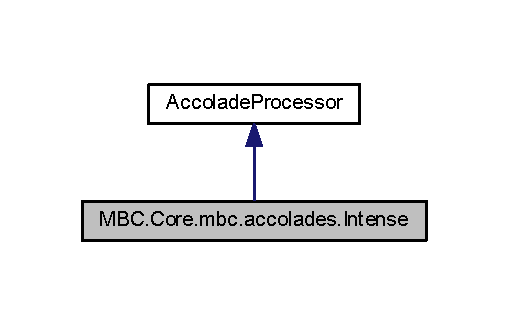
\includegraphics[width=244pt]{class_m_b_c_1_1_core_1_1mbc_1_1accolades_1_1_intense__inherit__graph}
\end{center}
\end{figure}


Collaboration diagram for M\-B\-C.\-Core.\-mbc.\-accolades.\-Intense\-:\nopagebreak
\begin{figure}[H]
\begin{center}
\leavevmode
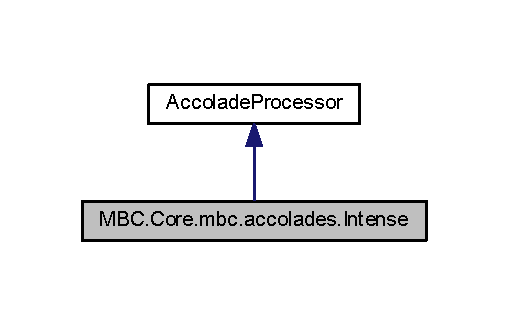
\includegraphics[width=244pt]{class_m_b_c_1_1_core_1_1mbc_1_1accolades_1_1_intense__coll__graph}
\end{center}
\end{figure}
\subsection*{Public Member Functions}
\begin{DoxyCompactItemize}
\item 
\hypertarget{class_m_b_c_1_1_core_1_1mbc_1_1accolades_1_1_intense_ad0177a4a8e91e17b2a08804eff068f0b}{Round\-Log.\-Round\-Accolade \hyperlink{class_m_b_c_1_1_core_1_1mbc_1_1accolades_1_1_intense_ad0177a4a8e91e17b2a08804eff068f0b}{Process} (\hyperlink{class_m_b_c_1_1_core_1_1_round_log_1_1_round_activity}{Round\-Log.\-Round\-Activity} a)}\label{class_m_b_c_1_1_core_1_1mbc_1_1accolades_1_1_intense_ad0177a4a8e91e17b2a08804eff068f0b}

\begin{DoxyCompactList}\small\item\em Process an activity\end{DoxyCompactList}\end{DoxyCompactItemize}


The documentation for this class was generated from the following file\-:\begin{DoxyCompactItemize}
\item 
M\-B\-C Core/accolades/Intense.\-cs\end{DoxyCompactItemize}

\hypertarget{class_m_b_c_1_1_core_1_1util_1_1_log}{\section{M\-B\-C.\-Core.\-util.\-Log Class Reference}
\label{class_m_b_c_1_1_core_1_1util_1_1_log}\index{M\-B\-C.\-Core.\-util.\-Log@{M\-B\-C.\-Core.\-util.\-Log}}
}


The \hyperlink{class_m_b_c_1_1_core_1_1util_1_1_log}{Log} class is used to monitor a stream or a file for log changes, and provides events for log monitoring. (C\-L\-I\-E\-N\-T) 


\subsection*{Public Member Functions}
\begin{DoxyCompactItemize}
\item 
\hypertarget{class_m_b_c_1_1_core_1_1util_1_1_log_a8af64f74500a37275589f3503d90279d}{delegate void {\bfseries Log\-Message\-Received} (\hyperlink{class_m_b_c_1_1_core_1_1util_1_1_log_message}{Log\-Message} msg)}\label{class_m_b_c_1_1_core_1_1util_1_1_log_a8af64f74500a37275589f3503d90279d}

\item 
\hypertarget{class_m_b_c_1_1_core_1_1util_1_1_log_a2cd8fbd24c6339b8d9c4855476dc29a1}{\hyperlink{class_m_b_c_1_1_core_1_1util_1_1_log_a2cd8fbd24c6339b8d9c4855476dc29a1}{Log} (Stream\-Reader read\-From)}\label{class_m_b_c_1_1_core_1_1util_1_1_log_a2cd8fbd24c6339b8d9c4855476dc29a1}

\begin{DoxyCompactList}\small\item\em This \hyperlink{class_m_b_c_1_1_core_1_1util_1_1_log}{Log} class constructor requires a stream to read from. Then, the constructor will begin creating a new thread to monitor the stream.\end{DoxyCompactList}\end{DoxyCompactItemize}
\subsection*{Events}
\begin{DoxyCompactItemize}
\item 
\hypertarget{class_m_b_c_1_1_core_1_1util_1_1_log_a536188a88d12672bb3489b9c34784831}{Log\-Message\-Received {\bfseries Log\-Message\-Received\-Event}}\label{class_m_b_c_1_1_core_1_1util_1_1_log_a536188a88d12672bb3489b9c34784831}

\end{DoxyCompactItemize}


\subsection{Detailed Description}
The \hyperlink{class_m_b_c_1_1_core_1_1util_1_1_log}{Log} class is used to monitor a stream or a file for log changes, and provides events for log monitoring. (C\-L\-I\-E\-N\-T)

The documentation for this class was generated from the following file\-:\begin{DoxyCompactItemize}
\item 
Core/util/logging/Log.\-cs\end{DoxyCompactItemize}

\hypertarget{class_m_b_c_1_1_core_1_1util_1_1_logger}{\section{M\-B\-C.\-Core.\-util.\-Logger Class Reference}
\label{class_m_b_c_1_1_core_1_1util_1_1_logger}\index{M\-B\-C.\-Core.\-util.\-Logger@{M\-B\-C.\-Core.\-util.\-Logger}}
}


Used for logging. 


\subsection*{Public Member Functions}
\begin{DoxyCompactItemize}
\item 
\hypertarget{class_m_b_c_1_1_core_1_1util_1_1_logger_ac2fdea5c1750f1dbc63fefde8bb0e12f}{{\bfseries Logger} (string n)}\label{class_m_b_c_1_1_core_1_1util_1_1_logger_ac2fdea5c1750f1dbc63fefde8bb0e12f}

\item 
\hypertarget{class_m_b_c_1_1_core_1_1util_1_1_logger_a21316aef85df8eb5decf285c50badfdc}{void \hyperlink{class_m_b_c_1_1_core_1_1util_1_1_logger_a21316aef85df8eb5decf285c50badfdc}{Add\-Output\-Stream} (Stream\-Writer s\-Out)}\label{class_m_b_c_1_1_core_1_1util_1_1_logger_a21316aef85df8eb5decf285c50badfdc}

\begin{DoxyCompactList}\small\item\em Attach a stream to this log, such as a file stream or a network stream.\end{DoxyCompactList}\item 
void \hyperlink{class_m_b_c_1_1_core_1_1util_1_1_logger_a9dbb38c93a6869f689516e8f3854981d}{Log} (string message)
\begin{DoxyCompactList}\small\item\em Prefix-\/enabled logging method. Use the prefixes beginning with an exclaimation mark (!) to specify a log message level. The message can be entered directly after the two characters.\par
 This is only a simple logging method.\par
 \end{DoxyCompactList}\item 
\hypertarget{class_m_b_c_1_1_core_1_1util_1_1_logger_ae4b2c81601b3af0189ca50c834268826}{void \hyperlink{class_m_b_c_1_1_core_1_1util_1_1_logger_ae4b2c81601b3af0189ca50c834268826}{Log} (string message, Log\-Message.\-Level lvl)}\label{class_m_b_c_1_1_core_1_1util_1_1_logger_ae4b2c81601b3af0189ca50c834268826}

\begin{DoxyCompactList}\small\item\em \hyperlink{class_m_b_c_1_1_core_1_1util_1_1_log}{Log} a message with the specified level. This will also immediately output to the attached streams within the same thread.\end{DoxyCompactList}\end{DoxyCompactItemize}


\subsection{Detailed Description}
Used for logging.

\subsection{Member Function Documentation}
\hypertarget{class_m_b_c_1_1_core_1_1util_1_1_logger_a9dbb38c93a6869f689516e8f3854981d}{\index{M\-B\-C\-::\-Core\-::util\-::\-Logger@{M\-B\-C\-::\-Core\-::util\-::\-Logger}!Log@{Log}}
\index{Log@{Log}!MBC::Core::util::Logger@{M\-B\-C\-::\-Core\-::util\-::\-Logger}}
\subsubsection[{Log}]{\setlength{\rightskip}{0pt plus 5cm}void M\-B\-C.\-Core.\-util.\-Logger.\-Log (
\begin{DoxyParamCaption}
\item[{string}]{message}
\end{DoxyParamCaption}
)}}\label{class_m_b_c_1_1_core_1_1util_1_1_logger_a9dbb38c93a6869f689516e8f3854981d}


Prefix-\/enabled logging method. Use the prefixes beginning with an exclaimation mark (!) to specify a log message level. The message can be entered directly after the two characters.\par
 This is only a simple logging method.\par
 


\begin{DoxyItemize}
\item 
\end{DoxyItemize}prefixes\-: !v -\/ Verbose !i -\/ Info !d -\/ Debug !w -\/ Warning !e -\/ Error !c -\/ Critical !f -\/ Fatal 

Here is the call graph for this function\-:
\nopagebreak
\begin{figure}[H]
\begin{center}
\leavevmode
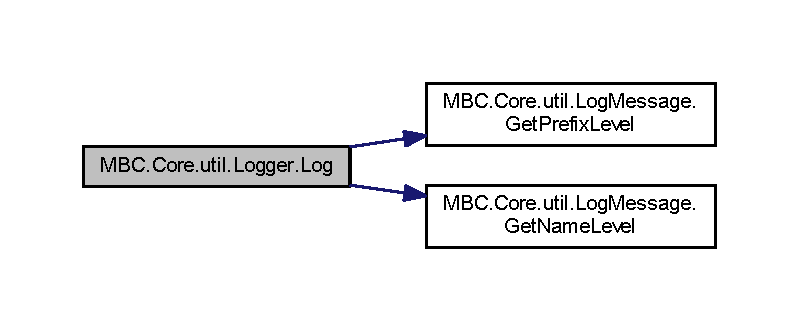
\includegraphics[width=350pt]{class_m_b_c_1_1_core_1_1util_1_1_logger_a9dbb38c93a6869f689516e8f3854981d_cgraph}
\end{center}
\end{figure}




The documentation for this class was generated from the following file\-:\begin{DoxyCompactItemize}
\item 
M\-B\-C Core/util/logging/Logger.\-cs\end{DoxyCompactItemize}

\hypertarget{class_m_b_c_1_1_core_1_1util_1_1_logger_manager}{\section{M\-B\-C.\-Core.\-util.\-Logger\-Manager Class Reference}
\label{class_m_b_c_1_1_core_1_1util_1_1_logger_manager}\index{M\-B\-C.\-Core.\-util.\-Logger\-Manager@{M\-B\-C.\-Core.\-util.\-Logger\-Manager}}
}
\subsection*{Static Public Member Functions}
\begin{DoxyCompactItemize}
\item 
static \hyperlink{class_m_b_c_1_1_core_1_1util_1_1_logger}{Logger} \hyperlink{class_m_b_c_1_1_core_1_1util_1_1_logger_manager_a8ec18cb07826e003bf2eb94ca672840f}{Get\-Logger} (string name)
\begin{DoxyCompactList}\small\item\em Use this function to select the \hyperlink{class_m_b_c_1_1_core_1_1util_1_1_logger}{Logger} class attached with a string\end{DoxyCompactList}\end{DoxyCompactItemize}


\subsection{Member Function Documentation}
\hypertarget{class_m_b_c_1_1_core_1_1util_1_1_logger_manager_a8ec18cb07826e003bf2eb94ca672840f}{\index{M\-B\-C\-::\-Core\-::util\-::\-Logger\-Manager@{M\-B\-C\-::\-Core\-::util\-::\-Logger\-Manager}!Get\-Logger@{Get\-Logger}}
\index{Get\-Logger@{Get\-Logger}!MBC::Core::util::LoggerManager@{M\-B\-C\-::\-Core\-::util\-::\-Logger\-Manager}}
\subsubsection[{Get\-Logger}]{\setlength{\rightskip}{0pt plus 5cm}static {\bf Logger} M\-B\-C.\-Core.\-util.\-Logger\-Manager.\-Get\-Logger (
\begin{DoxyParamCaption}
\item[{string}]{name}
\end{DoxyParamCaption}
)\hspace{0.3cm}{\ttfamily [static]}}}\label{class_m_b_c_1_1_core_1_1util_1_1_logger_manager_a8ec18cb07826e003bf2eb94ca672840f}


Use this function to select the \hyperlink{class_m_b_c_1_1_core_1_1util_1_1_logger}{Logger} class attached with a string

Use as \hyperlink{class_m_b_c_1_1_core_1_1util_1_1_logger_manager}{Logger\-Manager}\mbox{[}\char`\"{}\-A\-N\-Y\-\_\-\-N\-A\-M\-E\char`\"{}\mbox{]} to get \hyperlink{class_m_b_c_1_1_core_1_1util_1_1_logger}{Logger} objects. It will generate non-\/existing Loggers automatically.

The documentation for this class was generated from the following file\-:\begin{DoxyCompactItemize}
\item 
M\-B\-C Core/util/Logger\-Manager.\-cs\end{DoxyCompactItemize}

\hypertarget{class_m_b_c_1_1_core_1_1util_1_1_log_message}{\section{M\-B\-C.\-Core.\-util.\-Log\-Message Class Reference}
\label{class_m_b_c_1_1_core_1_1util_1_1_log_message}\index{M\-B\-C.\-Core.\-util.\-Log\-Message@{M\-B\-C.\-Core.\-util.\-Log\-Message}}
}


The \hyperlink{class_m_b_c_1_1_core_1_1util_1_1_log_message}{Log\-Message} class is used to describe a single log message to a \hyperlink{class_m_b_c_1_1_core_1_1util_1_1_log}{Log} object. 


\subsection*{Public Types}
\begin{DoxyCompactItemize}
\item 
enum {\bfseries Level} \{ \\*
{\bfseries Verbose}, 
{\bfseries Info}, 
{\bfseries Debug}, 
{\bfseries Warning}, 
\\*
{\bfseries Error}, 
{\bfseries Critical}, 
{\bfseries Fatal}
 \}
\end{DoxyCompactItemize}
\subsection*{Public Member Functions}
\begin{DoxyCompactItemize}
\item 
\hypertarget{class_m_b_c_1_1_core_1_1util_1_1_log_message_a28227ed3687ed1b74fd4553373d9caee}{{\bfseries Log\-Message} (string msg, Level lvl, Date\-Time time)}\label{class_m_b_c_1_1_core_1_1util_1_1_log_message_a28227ed3687ed1b74fd4553373d9caee}

\end{DoxyCompactItemize}
\subsection*{Static Public Member Functions}
\begin{DoxyCompactItemize}
\item 
\hypertarget{class_m_b_c_1_1_core_1_1util_1_1_log_message_a118fce73f3b41f40305c7e7efc687620}{static Log\-Message.\-Level \hyperlink{class_m_b_c_1_1_core_1_1util_1_1_log_message_a118fce73f3b41f40305c7e7efc687620}{Get\-Prefix\-Level} (string pre)}\label{class_m_b_c_1_1_core_1_1util_1_1_log_message_a118fce73f3b41f40305c7e7efc687620}

\begin{DoxyCompactList}\small\item\em Translates a prefix string into the corresponding \hyperlink{class_m_b_c_1_1_core_1_1util_1_1_log_message}{Log\-Message} Level. The string specified will be made into lowercase.\end{DoxyCompactList}\item 
\hypertarget{class_m_b_c_1_1_core_1_1util_1_1_log_message_a5826ddb8de3dbc2c294d5ea98756c911}{static Log\-Message.\-Level \hyperlink{class_m_b_c_1_1_core_1_1util_1_1_log_message_a5826ddb8de3dbc2c294d5ea98756c911}{Get\-Name\-Level} (string name)}\label{class_m_b_c_1_1_core_1_1util_1_1_log_message_a5826ddb8de3dbc2c294d5ea98756c911}

\begin{DoxyCompactList}\small\item\em Translates a name string into the corresponding \hyperlink{class_m_b_c_1_1_core_1_1util_1_1_log_message}{Log\-Message} Level.\end{DoxyCompactList}\end{DoxyCompactItemize}


\subsection{Detailed Description}
The \hyperlink{class_m_b_c_1_1_core_1_1util_1_1_log_message}{Log\-Message} class is used to describe a single log message to a \hyperlink{class_m_b_c_1_1_core_1_1util_1_1_log}{Log} object.

The documentation for this class was generated from the following file\-:\begin{DoxyCompactItemize}
\item 
Core/util/logging/Log\-Message.\-cs\end{DoxyCompactItemize}

\hypertarget{class_m_b_c_1_1_w_p_f_1_1_main_window}{\section{M\-B\-C.\-W\-P\-F.\-Main\-Window Class Reference}
\label{class_m_b_c_1_1_w_p_f_1_1_main_window}\index{M\-B\-C.\-W\-P\-F.\-Main\-Window@{M\-B\-C.\-W\-P\-F.\-Main\-Window}}
}


\hyperlink{class_m_b_c_1_1_w_p_f_1_1_main_window}{Main\-Window}  




Inheritance diagram for M\-B\-C.\-W\-P\-F.\-Main\-Window\-:
\nopagebreak
\begin{figure}[H]
\begin{center}
\leavevmode
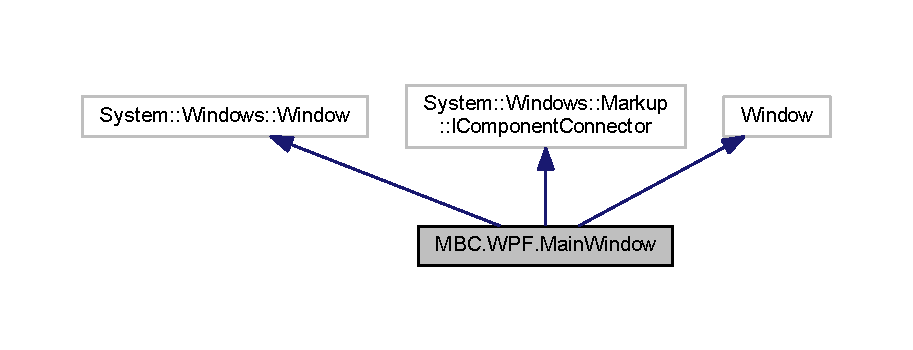
\includegraphics[width=350pt]{class_m_b_c_1_1_w_p_f_1_1_main_window__inherit__graph}
\end{center}
\end{figure}


Collaboration diagram for M\-B\-C.\-W\-P\-F.\-Main\-Window\-:
\nopagebreak
\begin{figure}[H]
\begin{center}
\leavevmode
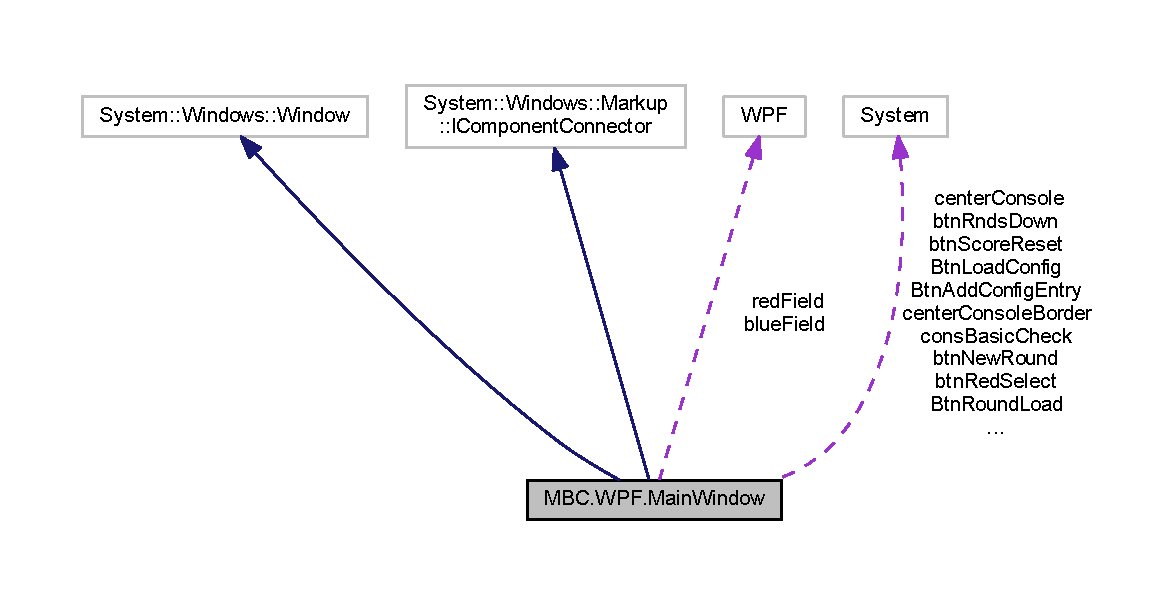
\includegraphics[width=350pt]{class_m_b_c_1_1_w_p_f_1_1_main_window__coll__graph}
\end{center}
\end{figure}
\subsection*{Public Member Functions}
\begin{DoxyCompactItemize}
\item 
void \hyperlink{class_m_b_c_1_1_w_p_f_1_1_main_window_af7a6d8874e20196c3db0d7987d97819f}{Initialize\-Component} ()
\begin{DoxyCompactList}\small\item\em Initialize\-Component \end{DoxyCompactList}\end{DoxyCompactItemize}


\subsection{Detailed Description}
\hyperlink{class_m_b_c_1_1_w_p_f_1_1_main_window}{Main\-Window} 



\subsection{Member Function Documentation}
\hypertarget{class_m_b_c_1_1_w_p_f_1_1_main_window_af7a6d8874e20196c3db0d7987d97819f}{\index{M\-B\-C\-::\-W\-P\-F\-::\-Main\-Window@{M\-B\-C\-::\-W\-P\-F\-::\-Main\-Window}!Initialize\-Component@{Initialize\-Component}}
\index{Initialize\-Component@{Initialize\-Component}!MBC::WPF::MainWindow@{M\-B\-C\-::\-W\-P\-F\-::\-Main\-Window}}
\subsubsection[{Initialize\-Component}]{\setlength{\rightskip}{0pt plus 5cm}void M\-B\-C.\-W\-P\-F.\-Main\-Window.\-Initialize\-Component (
\begin{DoxyParamCaption}
{}
\end{DoxyParamCaption}
)}}\label{class_m_b_c_1_1_w_p_f_1_1_main_window_af7a6d8874e20196c3db0d7987d97819f}


Initialize\-Component 



The documentation for this class was generated from the following file\-:\begin{DoxyCompactItemize}
\item 
App\-W\-P\-F/obj/x86/\-Debug/Main\-Window.\-g.\-cs\end{DoxyCompactItemize}

\hypertarget{class_m_b_c_1_1_g_l_1_1_program}{\section{M\-B\-C.\-G\-L.\-Program Class Reference}
\label{class_m_b_c_1_1_g_l_1_1_program}\index{M\-B\-C.\-G\-L.\-Program@{M\-B\-C.\-G\-L.\-Program}}
}


The documentation for this class was generated from the following file\-:\begin{DoxyCompactItemize}
\item 
M\-B\-C 3\-D/Program.\-cs\end{DoxyCompactItemize}

\hypertarget{class_m_b_c_1_1_terminal_1_1_program}{\section{M\-B\-C.\-Terminal.\-Program Class Reference}
\label{class_m_b_c_1_1_terminal_1_1_program}\index{M\-B\-C.\-Terminal.\-Program@{M\-B\-C.\-Terminal.\-Program}}
}


The documentation for this class was generated from the following file\-:\begin{DoxyCompactItemize}
\item 
M\-B\-C Terminal/Program.\-cs\end{DoxyCompactItemize}

\hypertarget{class_m_b_c_1_1_bots_1_1_random_bot}{\section{M\-B\-C.\-Bots.\-Random\-Bot Class Reference}
\label{class_m_b_c_1_1_bots_1_1_random_bot}\index{M\-B\-C.\-Bots.\-Random\-Bot@{M\-B\-C.\-Bots.\-Random\-Bot}}
}


Inheritance diagram for M\-B\-C.\-Bots.\-Random\-Bot\-:\nopagebreak
\begin{figure}[H]
\begin{center}
\leavevmode
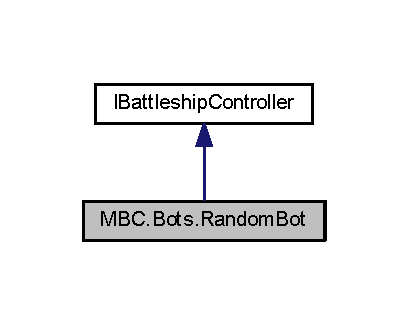
\includegraphics[width=196pt]{class_m_b_c_1_1_bots_1_1_random_bot__inherit__graph}
\end{center}
\end{figure}


Collaboration diagram for M\-B\-C.\-Bots.\-Random\-Bot\-:\nopagebreak
\begin{figure}[H]
\begin{center}
\leavevmode
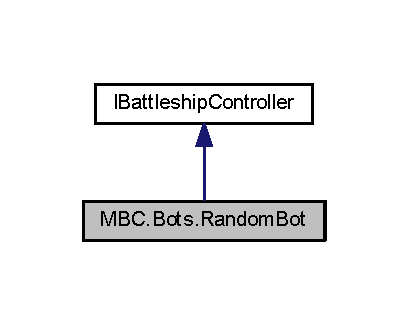
\includegraphics[width=196pt]{class_m_b_c_1_1_bots_1_1_random_bot__coll__graph}
\end{center}
\end{figure}
\subsection*{Public Member Functions}
\begin{DoxyCompactItemize}
\item 
\hypertarget{class_m_b_c_1_1_bots_1_1_random_bot_a3547fdf31c01dc6946e907a54a24da7e}{void {\bfseries New\-Game} (Size size, Time\-Span time\-Span, Random rand)}\label{class_m_b_c_1_1_bots_1_1_random_bot_a3547fdf31c01dc6946e907a54a24da7e}

\item 
\hypertarget{class_m_b_c_1_1_bots_1_1_random_bot_aa8bffd9cb890f0061686efda7f5613fe}{void {\bfseries Place\-Ships} (Read\-Only\-Collection$<$ \hyperlink{class_m_b_c_1_1_core_1_1_ship}{Ship} $>$ ships)}\label{class_m_b_c_1_1_bots_1_1_random_bot_aa8bffd9cb890f0061686efda7f5613fe}

\item 
\hypertarget{class_m_b_c_1_1_bots_1_1_random_bot_a4bdce7f14e3e9cb4e0c066d8240a764e}{Point {\bfseries Get\-Shot} ()}\label{class_m_b_c_1_1_bots_1_1_random_bot_a4bdce7f14e3e9cb4e0c066d8240a764e}

\item 
\hypertarget{class_m_b_c_1_1_bots_1_1_random_bot_a0a4365d6e3f2100c96776aa9b8771c33}{void {\bfseries New\-Match} (string opponent)}\label{class_m_b_c_1_1_bots_1_1_random_bot_a0a4365d6e3f2100c96776aa9b8771c33}

\item 
\hypertarget{class_m_b_c_1_1_bots_1_1_random_bot_a3414498efd36aeadba60cabde19466b9}{void {\bfseries Opponent\-Shot} (Point shot)}\label{class_m_b_c_1_1_bots_1_1_random_bot_a3414498efd36aeadba60cabde19466b9}

\item 
\hypertarget{class_m_b_c_1_1_bots_1_1_random_bot_ad7212214b2a50863d41b9dbefd71e51d}{void {\bfseries Shot\-Hit} (Point shot, bool sunk)}\label{class_m_b_c_1_1_bots_1_1_random_bot_ad7212214b2a50863d41b9dbefd71e51d}

\item 
\hypertarget{class_m_b_c_1_1_bots_1_1_random_bot_aae077027406736b2097d7b778cde90fa}{void {\bfseries Shot\-Miss} (Point shot)}\label{class_m_b_c_1_1_bots_1_1_random_bot_aae077027406736b2097d7b778cde90fa}

\item 
\hypertarget{class_m_b_c_1_1_bots_1_1_random_bot_ac782e5e79375861b37e323f43e109862}{void {\bfseries Game\-Won} ()}\label{class_m_b_c_1_1_bots_1_1_random_bot_ac782e5e79375861b37e323f43e109862}

\item 
\hypertarget{class_m_b_c_1_1_bots_1_1_random_bot_a6c6bf2d1f760ca43f26fce92c3be5762}{void {\bfseries Game\-Lost} ()}\label{class_m_b_c_1_1_bots_1_1_random_bot_a6c6bf2d1f760ca43f26fce92c3be5762}

\item 
\hypertarget{class_m_b_c_1_1_bots_1_1_random_bot_a1fed13a8154ba2b63f76abf85a60f782}{void {\bfseries Match\-Over} ()}\label{class_m_b_c_1_1_bots_1_1_random_bot_a1fed13a8154ba2b63f76abf85a60f782}

\end{DoxyCompactItemize}
\subsection*{Properties}
\begin{DoxyCompactItemize}
\item 
\hypertarget{class_m_b_c_1_1_bots_1_1_random_bot_a09a9e4b4ea05bea001bebd2819e49999}{string {\bfseries Name}\hspace{0.3cm}{\ttfamily  \mbox{[}get\mbox{]}}}\label{class_m_b_c_1_1_bots_1_1_random_bot_a09a9e4b4ea05bea001bebd2819e49999}

\item 
\hypertarget{class_m_b_c_1_1_bots_1_1_random_bot_a32a130d474e7930e1bc2942e5697987f}{Version {\bfseries Version}\hspace{0.3cm}{\ttfamily  \mbox{[}get\mbox{]}}}\label{class_m_b_c_1_1_bots_1_1_random_bot_a32a130d474e7930e1bc2942e5697987f}

\end{DoxyCompactItemize}


The documentation for this class was generated from the following file\-:\begin{DoxyCompactItemize}
\item 
M\-B\-C Bots/Random\-Opponent.\-cs\end{DoxyCompactItemize}

\hypertarget{class_m_b_c_1_1_terminal_1_1_result_state}{\section{M\-B\-C.\-Terminal.\-Result\-State Class Reference}
\label{class_m_b_c_1_1_terminal_1_1_result_state}\index{M\-B\-C.\-Terminal.\-Result\-State@{M\-B\-C.\-Terminal.\-Result\-State}}
}


Inheritance diagram for M\-B\-C.\-Terminal.\-Result\-State\-:\nopagebreak
\begin{figure}[H]
\begin{center}
\leavevmode
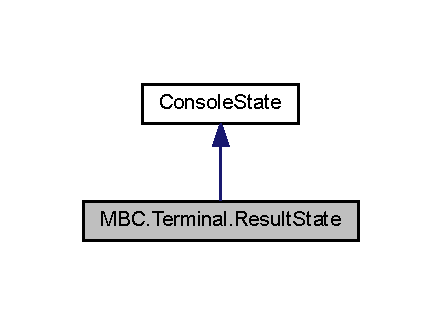
\includegraphics[width=212pt]{class_m_b_c_1_1_terminal_1_1_result_state__inherit__graph}
\end{center}
\end{figure}


Collaboration diagram for M\-B\-C.\-Terminal.\-Result\-State\-:\nopagebreak
\begin{figure}[H]
\begin{center}
\leavevmode
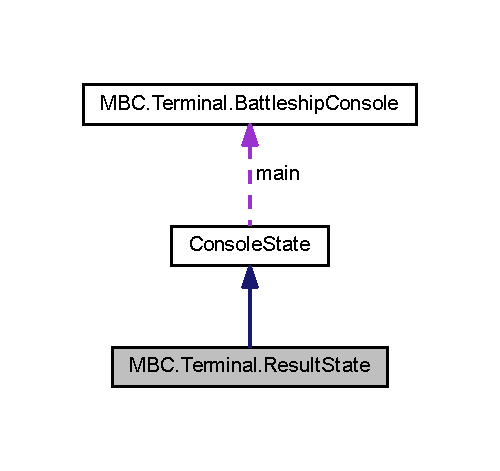
\includegraphics[width=240pt]{class_m_b_c_1_1_terminal_1_1_result_state__coll__graph}
\end{center}
\end{figure}
\subsection*{Public Member Functions}
\begin{DoxyCompactItemize}
\item 
\hypertarget{class_m_b_c_1_1_terminal_1_1_result_state_a2026218800c999e2e3ce86279cd24035}{{\bfseries Result\-State} (\hyperlink{class_m_b_c_1_1_terminal_1_1_battleship_console}{Battleship\-Console} main, Dictionary$<$ \hyperlink{interface_m_b_c_1_1_core_1_1_i_battleship_controller}{I\-Battleship\-Controller}, int $>$ results)}\label{class_m_b_c_1_1_terminal_1_1_result_state_a2026218800c999e2e3ce86279cd24035}

\end{DoxyCompactItemize}
\subsection*{Protected Member Functions}
\begin{DoxyCompactItemize}
\item 
\hypertarget{class_m_b_c_1_1_terminal_1_1_result_state_aa3b4aff3c8ecbc6ef612dd9b3bcf1fff}{override void \hyperlink{class_m_b_c_1_1_terminal_1_1_result_state_aa3b4aff3c8ecbc6ef612dd9b3bcf1fff}{State\-Display} ()}\label{class_m_b_c_1_1_terminal_1_1_result_state_aa3b4aff3c8ecbc6ef612dd9b3bcf1fff}

\begin{DoxyCompactList}\small\item\em Overridden to provide specific printing related to the subclass.\end{DoxyCompactList}\item 
override \hyperlink{class_m_b_c_1_1_terminal_1_1_console_state}{Console\-State} \hyperlink{class_m_b_c_1_1_terminal_1_1_result_state_a530fa6f7b36a58d0ffa09fab3048508a}{Response} (string input)
\begin{DoxyCompactList}\small\item\em Called when input is not handled by the base class.\end{DoxyCompactList}\end{DoxyCompactItemize}
\subsection*{Additional Inherited Members}


\subsection{Member Function Documentation}
\hypertarget{class_m_b_c_1_1_terminal_1_1_result_state_a530fa6f7b36a58d0ffa09fab3048508a}{\index{M\-B\-C\-::\-Terminal\-::\-Result\-State@{M\-B\-C\-::\-Terminal\-::\-Result\-State}!Response@{Response}}
\index{Response@{Response}!MBC::Terminal::ResultState@{M\-B\-C\-::\-Terminal\-::\-Result\-State}}
\subsubsection[{Response}]{\setlength{\rightskip}{0pt plus 5cm}override {\bf Console\-State} M\-B\-C.\-Terminal.\-Result\-State.\-Response (
\begin{DoxyParamCaption}
\item[{string}]{input}
\end{DoxyParamCaption}
)\hspace{0.3cm}{\ttfamily [protected]}, {\ttfamily [virtual]}}}\label{class_m_b_c_1_1_terminal_1_1_result_state_a530fa6f7b36a58d0ffa09fab3048508a}


Called when input is not handled by the base class.


\begin{DoxyParams}{Parameters}
{\em input} & The string entered by the user\\
\hline
\end{DoxyParams}
\begin{DoxyReturn}{Returns}
The implementing class, null, or a new \hyperlink{class_m_b_c_1_1_terminal_1_1_console_state}{Console\-State} object. null will end the program.
\end{DoxyReturn}


Implements \hyperlink{class_m_b_c_1_1_terminal_1_1_console_state_a93d6eee582913a59d10348cdc8ef4248}{M\-B\-C.\-Terminal.\-Console\-State}.



The documentation for this class was generated from the following file\-:\begin{DoxyCompactItemize}
\item 
M\-B\-C Terminal/Result\-State.\-cs\end{DoxyCompactItemize}

\hypertarget{class_m_b_c_1_1_core_1_1_round_log_1_1_round_activity}{\section{M\-B\-C.\-Core.\-Round\-Log.\-Round\-Activity Class Reference}
\label{class_m_b_c_1_1_core_1_1_round_log_1_1_round_activity}\index{M\-B\-C.\-Core.\-Round\-Log.\-Round\-Activity@{M\-B\-C.\-Core.\-Round\-Log.\-Round\-Activity}}
}


A \hyperlink{class_m_b_c_1_1_core_1_1_round_log_1_1_round_activity}{Round\-Activity} contains information about a single event in a round. Multiple \hyperlink{class_m_b_c_1_1_core_1_1_round_log_1_1_round_activity}{Round\-Activity} objects make up a \hyperlink{class_m_b_c_1_1_core_1_1_round_log}{Round\-Log}.  




Collaboration diagram for M\-B\-C.\-Core.\-Round\-Log.\-Round\-Activity\-:
\nopagebreak
\begin{figure}[H]
\begin{center}
\leavevmode
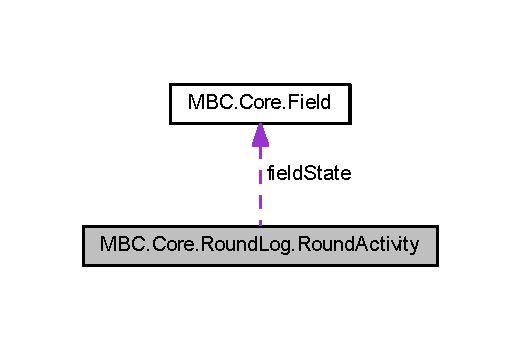
\includegraphics[width=250pt]{class_m_b_c_1_1_core_1_1_round_log_1_1_round_activity__coll__graph}
\end{center}
\end{figure}
\subsection*{Public Member Functions}
\begin{DoxyCompactItemize}
\item 
\hypertarget{class_m_b_c_1_1_core_1_1_round_log_1_1_round_activity_afa28bd29e4c11ad135efc72c1cc2f499}{\hyperlink{class_m_b_c_1_1_core_1_1_round_log_1_1_round_activity_afa28bd29e4c11ad135efc72c1cc2f499}{Round\-Activity} (int bc, \hyperlink{class_m_b_c_1_1_core_1_1_round_log_af3f9f76d90fb391108dd1eaeaeae27e4}{Round\-Action} a)}\label{class_m_b_c_1_1_core_1_1_round_log_1_1_round_activity_afa28bd29e4c11ad135efc72c1cc2f499}

\begin{DoxyCompactList}\small\item\em The minimal constructor for a \hyperlink{class_m_b_c_1_1_core_1_1_round_log_1_1_round_activity}{Round\-Activity} object. Each \hyperlink{class_m_b_c_1_1_core_1_1_round_log_1_1_round_activity}{Round\-Activity} requires that a \hyperlink{class_m_b_c_1_1_core_1_1_controller}{Controller} index and Round\-Action be specified. Other parameters are optional. \end{DoxyCompactList}\item 
\hypertarget{class_m_b_c_1_1_core_1_1_round_log_1_1_round_activity_a88d7690a89cdcf004b0bf98bd851f865}{{\bfseries Round\-Activity} (string info, int bc, \hyperlink{class_m_b_c_1_1_core_1_1_round_log_af3f9f76d90fb391108dd1eaeaeae27e4}{Round\-Action} a)}\label{class_m_b_c_1_1_core_1_1_round_log_1_1_round_activity_a88d7690a89cdcf004b0bf98bd851f865}

\item 
\hypertarget{class_m_b_c_1_1_core_1_1_round_log_1_1_round_activity_aa70dc49936b51e6afdee215ef284d3bb}{{\bfseries Round\-Activity} (string info, int bc, \hyperlink{class_m_b_c_1_1_core_1_1_round_log_af3f9f76d90fb391108dd1eaeaeae27e4}{Round\-Action} a, long time)}\label{class_m_b_c_1_1_core_1_1_round_log_1_1_round_activity_aa70dc49936b51e6afdee215ef284d3bb}

\item 
\hypertarget{class_m_b_c_1_1_core_1_1_round_log_1_1_round_activity_af2a43e61c9bf543f45c056f66b3c48e5}{{\bfseries Round\-Activity} (string info, int bc, \hyperlink{class_m_b_c_1_1_core_1_1_round_log_af3f9f76d90fb391108dd1eaeaeae27e4}{Round\-Action} a, long time, \hyperlink{class_m_b_c_1_1_core_1_1_field}{Field} state)}\label{class_m_b_c_1_1_core_1_1_round_log_1_1_round_activity_af2a43e61c9bf543f45c056f66b3c48e5}

\item 
\hypertarget{class_m_b_c_1_1_core_1_1_round_log_1_1_round_activity_a46fdc053d4d185227893de422d2a4ba0}{void \hyperlink{class_m_b_c_1_1_core_1_1_round_log_1_1_round_activity_a46fdc053d4d185227893de422d2a4ba0}{Add\-Accolade} (\hyperlink{class_m_b_c_1_1_core_1_1_round_log_a4060830ca7135aa755ec5b6d24aa30e6}{Round\-Accolade} acc)}\label{class_m_b_c_1_1_core_1_1_round_log_1_1_round_activity_a46fdc053d4d185227893de422d2a4ba0}

\begin{DoxyCompactList}\small\item\em Adds an accolade associated with this \hyperlink{class_m_b_c_1_1_core_1_1_round_log_1_1_round_activity}{Round\-Activity}. Not recommended for use outside of the \hyperlink{class_m_b_c_1_1_core_1_1_round_log}{Round\-Log} object.\end{DoxyCompactList}\end{DoxyCompactItemize}
\subsection*{Public Attributes}
\begin{DoxyCompactItemize}
\item 
\hypertarget{class_m_b_c_1_1_core_1_1_round_log_1_1_round_activity_a93245160332d9eba203f366e9f6c7b40}{string {\bfseries activity\-Info}}\label{class_m_b_c_1_1_core_1_1_round_log_1_1_round_activity_a93245160332d9eba203f366e9f6c7b40}

\item 
\hypertarget{class_m_b_c_1_1_core_1_1_round_log_1_1_round_activity_a9621add554c3937e5dd83b64d6783ebd}{int {\bfseries ibc}}\label{class_m_b_c_1_1_core_1_1_round_log_1_1_round_activity_a9621add554c3937e5dd83b64d6783ebd}

\item 
\hypertarget{class_m_b_c_1_1_core_1_1_round_log_1_1_round_activity_af5aa39bdbfc08d5d91d1e78778169390}{\hyperlink{class_m_b_c_1_1_core_1_1_round_log_af3f9f76d90fb391108dd1eaeaeae27e4}{Round\-Action} {\bfseries action}}\label{class_m_b_c_1_1_core_1_1_round_log_1_1_round_activity_af5aa39bdbfc08d5d91d1e78778169390}

\item 
\hypertarget{class_m_b_c_1_1_core_1_1_round_log_1_1_round_activity_a41e76ac7f84c694a03a2d6deae2dd2e5}{long {\bfseries time\-Elapsed}}\label{class_m_b_c_1_1_core_1_1_round_log_1_1_round_activity_a41e76ac7f84c694a03a2d6deae2dd2e5}

\item 
\hypertarget{class_m_b_c_1_1_core_1_1_round_log_1_1_round_activity_ac8200bb672e193945d5cac7ad3bcfd5c}{List$<$ \hyperlink{class_m_b_c_1_1_core_1_1_round_log_a4060830ca7135aa755ec5b6d24aa30e6}{Round\-Accolade} $>$ {\bfseries accolade\-Timelined}}\label{class_m_b_c_1_1_core_1_1_round_log_1_1_round_activity_ac8200bb672e193945d5cac7ad3bcfd5c}

\item 
\hypertarget{class_m_b_c_1_1_core_1_1_round_log_1_1_round_activity_a007bff7b101c4416edae38eaa7590c71}{\hyperlink{class_m_b_c_1_1_core_1_1_field}{Field} {\bfseries field\-State}}\label{class_m_b_c_1_1_core_1_1_round_log_1_1_round_activity_a007bff7b101c4416edae38eaa7590c71}

\end{DoxyCompactItemize}
\subsection*{Static Public Attributes}
\begin{DoxyCompactItemize}
\item 
\hypertarget{class_m_b_c_1_1_core_1_1_round_log_1_1_round_activity_af8458e6721eb85d6155a1fc5d81beb6d}{static string {\bfseries Reason\-\_\-\-Timeout} = \char`\"{}Timeout\char`\"{}}\label{class_m_b_c_1_1_core_1_1_round_log_1_1_round_activity_af8458e6721eb85d6155a1fc5d81beb6d}

\end{DoxyCompactItemize}


\subsection{Detailed Description}
A \hyperlink{class_m_b_c_1_1_core_1_1_round_log_1_1_round_activity}{Round\-Activity} contains information about a single event in a round. Multiple \hyperlink{class_m_b_c_1_1_core_1_1_round_log_1_1_round_activity}{Round\-Activity} objects make up a \hyperlink{class_m_b_c_1_1_core_1_1_round_log}{Round\-Log}. 

See the public member variable documentation to see the information that is stored in a \hyperlink{class_m_b_c_1_1_core_1_1_round_log_1_1_round_activity}{Round\-Activity}. 

The documentation for this class was generated from the following file\-:\begin{DoxyCompactItemize}
\item 
Core/Round\-Log.\-cs\end{DoxyCompactItemize}

\hypertarget{class_m_b_c_1_1_w_p_f_1_1_main_window_1_1_round_activity_entry}{\section{M\-B\-C.\-W\-P\-F.\-Main\-Window.\-Round\-Activity\-Entry Class Reference}
\label{class_m_b_c_1_1_w_p_f_1_1_main_window_1_1_round_activity_entry}\index{M\-B\-C.\-W\-P\-F.\-Main\-Window.\-Round\-Activity\-Entry@{M\-B\-C.\-W\-P\-F.\-Main\-Window.\-Round\-Activity\-Entry}}
}
\subsection*{Public Attributes}
\begin{DoxyCompactItemize}
\item 
\hypertarget{class_m_b_c_1_1_w_p_f_1_1_main_window_1_1_round_activity_entry_af6e27c24a5e0791ed05c630bebc6e10b}{string {\bfseries Number}}\label{class_m_b_c_1_1_w_p_f_1_1_main_window_1_1_round_activity_entry_af6e27c24a5e0791ed05c630bebc6e10b}

\item 
\hypertarget{class_m_b_c_1_1_w_p_f_1_1_main_window_1_1_round_activity_entry_aea96424ed99783f4d568367eb0361d2f}{string {\bfseries Action}}\label{class_m_b_c_1_1_w_p_f_1_1_main_window_1_1_round_activity_entry_aea96424ed99783f4d568367eb0361d2f}

\item 
\hypertarget{class_m_b_c_1_1_w_p_f_1_1_main_window_1_1_round_activity_entry_abfd5d18a30b5b7ec5568c22cfff36212}{string {\bfseries Controller\-Name}}\label{class_m_b_c_1_1_w_p_f_1_1_main_window_1_1_round_activity_entry_abfd5d18a30b5b7ec5568c22cfff36212}

\item 
\hypertarget{class_m_b_c_1_1_w_p_f_1_1_main_window_1_1_round_activity_entry_aa1a2ec80f45be5d265e5c9d22ba0d7f7}{string {\bfseries Message}}\label{class_m_b_c_1_1_w_p_f_1_1_main_window_1_1_round_activity_entry_aa1a2ec80f45be5d265e5c9d22ba0d7f7}

\item 
\hypertarget{class_m_b_c_1_1_w_p_f_1_1_main_window_1_1_round_activity_entry_a883afba30eab544c6294067892404a43}{string {\bfseries Time}}\label{class_m_b_c_1_1_w_p_f_1_1_main_window_1_1_round_activity_entry_a883afba30eab544c6294067892404a43}

\item 
\hypertarget{class_m_b_c_1_1_w_p_f_1_1_main_window_1_1_round_activity_entry_a3c686ce94c9514d9c974a7e8898b2109}{Grid {\bfseries Accolades}}\label{class_m_b_c_1_1_w_p_f_1_1_main_window_1_1_round_activity_entry_a3c686ce94c9514d9c974a7e8898b2109}

\item 
\hypertarget{class_m_b_c_1_1_w_p_f_1_1_main_window_1_1_round_activity_entry_adf003a8df551703a86d33cf9f1558377}{Color {\bfseries Color}}\label{class_m_b_c_1_1_w_p_f_1_1_main_window_1_1_round_activity_entry_adf003a8df551703a86d33cf9f1558377}

\end{DoxyCompactItemize}


The documentation for this class was generated from the following file\-:\begin{DoxyCompactItemize}
\item 
M\-B\-C W\-P\-F/Main\-Window.\-xaml.\-cs\end{DoxyCompactItemize}

\hypertarget{class_m_b_c_1_1_w_p_f_1_1_main_window_1_1_round_entry}{\section{M\-B\-C.\-W\-P\-F.\-Main\-Window.\-Round\-Entry Class Reference}
\label{class_m_b_c_1_1_w_p_f_1_1_main_window_1_1_round_entry}\index{M\-B\-C.\-W\-P\-F.\-Main\-Window.\-Round\-Entry@{M\-B\-C.\-W\-P\-F.\-Main\-Window.\-Round\-Entry}}
}
\subsection*{Public Attributes}
\begin{DoxyCompactItemize}
\item 
\hypertarget{class_m_b_c_1_1_w_p_f_1_1_main_window_1_1_round_entry_ac8491f1bf15d2fcb9ebd151c5efa3d77}{string {\bfseries Number}}\label{class_m_b_c_1_1_w_p_f_1_1_main_window_1_1_round_entry_ac8491f1bf15d2fcb9ebd151c5efa3d77}

\item 
\hypertarget{class_m_b_c_1_1_w_p_f_1_1_main_window_1_1_round_entry_aaca7d42e0063db62092deff7ec7a4668}{string {\bfseries Victor}}\label{class_m_b_c_1_1_w_p_f_1_1_main_window_1_1_round_entry_aaca7d42e0063db62092deff7ec7a4668}

\end{DoxyCompactItemize}


The documentation for this class was generated from the following file\-:\begin{DoxyCompactItemize}
\item 
M\-B\-C W\-P\-F/Main\-Window.\-xaml.\-cs\end{DoxyCompactItemize}

\hypertarget{class_m_b_c_1_1_core_1_1_round_log}{\section{M\-B\-C.\-Core.\-Round\-Log Class Reference}
\label{class_m_b_c_1_1_core_1_1_round_log}\index{M\-B\-C.\-Core.\-Round\-Log@{M\-B\-C.\-Core.\-Round\-Log}}
}


Keeps a log of a battleship competition round. 


\subsection*{Classes}
\begin{DoxyCompactItemize}
\item 
class \hyperlink{class_m_b_c_1_1_core_1_1_round_log_1_1_round_activity}{Round\-Activity}
\begin{DoxyCompactList}\small\item\em Defines a round action record\end{DoxyCompactList}\end{DoxyCompactItemize}
\subsection*{Public Types}
\begin{DoxyCompactItemize}
\item 
enum {\bfseries Round\-Action} \{ \\*
{\bfseries Shot\-And\-Miss}, 
{\bfseries Shot\-And\-Hit}, 
{\bfseries Ship\-Destroyed}, 
{\bfseries Round\-Begin}, 
\\*
{\bfseries Round\-End}, 
{\bfseries Ships\-Placed}, 
{\bfseries Won}, 
{\bfseries Lost}
 \}
\item 
enum {\bfseries Round\-Accolade} \{ \\*
{\bfseries Head\-To\-Head}, 
{\bfseries Domination}, 
{\bfseries Comeback}, 
{\bfseries Fast}, 
\\*
{\bfseries Slow}, 
{\bfseries Intense}, 
{\bfseries Stupid}, 
{\bfseries None}
 \}
\end{DoxyCompactItemize}
\subsection*{Public Member Functions}
\begin{DoxyCompactItemize}
\item 
\hypertarget{class_m_b_c_1_1_core_1_1_round_log_a50d3d5c41078aa520500ca86dd5694ab}{\hyperlink{class_m_b_c_1_1_core_1_1_round_log_a50d3d5c41078aa520500ca86dd5694ab}{Round\-Log} ()}\label{class_m_b_c_1_1_core_1_1_round_log_a50d3d5c41078aa520500ca86dd5694ab}

\begin{DoxyCompactList}\small\item\em Initializes the action processors\end{DoxyCompactList}\item 
\hypertarget{class_m_b_c_1_1_core_1_1_round_log_ad5114bea3e605c3587033cc4b9db6aa7}{void \hyperlink{class_m_b_c_1_1_core_1_1_round_log_ad5114bea3e605c3587033cc4b9db6aa7}{Reset\-Iterator} ()}\label{class_m_b_c_1_1_core_1_1_round_log_ad5114bea3e605c3587033cc4b9db6aa7}

\begin{DoxyCompactList}\small\item\em Starts counting the actions from zero again\end{DoxyCompactList}\item 
\hyperlink{class_m_b_c_1_1_core_1_1_round_log_1_1_round_activity}{Round\-Activity} \hyperlink{class_m_b_c_1_1_core_1_1_round_log_a14deb5b327e8c77d3535e342701711d9}{Get\-At} (int idx)
\item 
int \hyperlink{class_m_b_c_1_1_core_1_1_round_log_a389bd537cf73c73998e0a789961d7536}{Get\-Activity\-Count} ()
\item 
\hyperlink{class_m_b_c_1_1_core_1_1_round_log_1_1_round_activity}{Round\-Activity} \hyperlink{class_m_b_c_1_1_core_1_1_round_log_a02c4c7d407ff609478505d28ff20f884}{Get\-Next} ()
\item 
\hypertarget{class_m_b_c_1_1_core_1_1_round_log_a0bb405409acf2b889d714bbff68abc94}{void \hyperlink{class_m_b_c_1_1_core_1_1_round_log_a0bb405409acf2b889d714bbff68abc94}{Put\-Action} (\hyperlink{class_m_b_c_1_1_core_1_1_round_log_1_1_round_activity}{Round\-Activity} action)}\label{class_m_b_c_1_1_core_1_1_round_log_a0bb405409acf2b889d714bbff68abc94}

\begin{DoxyCompactList}\small\item\em Adds a constructed action to the list of activities recorded. Once the round end action has been appended, do not use this function anymore.\end{DoxyCompactList}\end{DoxyCompactItemize}


\subsection{Detailed Description}
Keeps a log of a battleship competition round.

\subsection{Member Function Documentation}
\hypertarget{class_m_b_c_1_1_core_1_1_round_log_a389bd537cf73c73998e0a789961d7536}{\index{M\-B\-C\-::\-Core\-::\-Round\-Log@{M\-B\-C\-::\-Core\-::\-Round\-Log}!Get\-Activity\-Count@{Get\-Activity\-Count}}
\index{Get\-Activity\-Count@{Get\-Activity\-Count}!MBC::Core::RoundLog@{M\-B\-C\-::\-Core\-::\-Round\-Log}}
\subsubsection[{Get\-Activity\-Count}]{\setlength{\rightskip}{0pt plus 5cm}int M\-B\-C.\-Core.\-Round\-Log.\-Get\-Activity\-Count (
\begin{DoxyParamCaption}
{}
\end{DoxyParamCaption}
)}}\label{class_m_b_c_1_1_core_1_1_round_log_a389bd537cf73c73998e0a789961d7536}
\begin{DoxyReturn}{Returns}
The number of actions recorded in this round
\end{DoxyReturn}
\hypertarget{class_m_b_c_1_1_core_1_1_round_log_a14deb5b327e8c77d3535e342701711d9}{\index{M\-B\-C\-::\-Core\-::\-Round\-Log@{M\-B\-C\-::\-Core\-::\-Round\-Log}!Get\-At@{Get\-At}}
\index{Get\-At@{Get\-At}!MBC::Core::RoundLog@{M\-B\-C\-::\-Core\-::\-Round\-Log}}
\subsubsection[{Get\-At}]{\setlength{\rightskip}{0pt plus 5cm}{\bf Round\-Activity} M\-B\-C.\-Core.\-Round\-Log.\-Get\-At (
\begin{DoxyParamCaption}
\item[{int}]{idx}
\end{DoxyParamCaption}
)}}\label{class_m_b_c_1_1_core_1_1_round_log_a14deb5b327e8c77d3535e342701711d9}
\begin{DoxyReturn}{Returns}
The activity at the specified action idx
\end{DoxyReturn}
\hypertarget{class_m_b_c_1_1_core_1_1_round_log_a02c4c7d407ff609478505d28ff20f884}{\index{M\-B\-C\-::\-Core\-::\-Round\-Log@{M\-B\-C\-::\-Core\-::\-Round\-Log}!Get\-Next@{Get\-Next}}
\index{Get\-Next@{Get\-Next}!MBC::Core::RoundLog@{M\-B\-C\-::\-Core\-::\-Round\-Log}}
\subsubsection[{Get\-Next}]{\setlength{\rightskip}{0pt plus 5cm}{\bf Round\-Activity} M\-B\-C.\-Core.\-Round\-Log.\-Get\-Next (
\begin{DoxyParamCaption}
{}
\end{DoxyParamCaption}
)}}\label{class_m_b_c_1_1_core_1_1_round_log_a02c4c7d407ff609478505d28ff20f884}
\begin{DoxyReturn}{Returns}
The next action record to read$<$/return$>$ 
\end{DoxyReturn}


The documentation for this class was generated from the following file\-:\begin{DoxyCompactItemize}
\item 
M\-B\-C Core/Round\-Log.\-cs\end{DoxyCompactItemize}

\hypertarget{class_m_b_c_1_1_terminal_1_1_selector_state}{\section{M\-B\-C.\-Terminal.\-Selector\-State Class Reference}
\label{class_m_b_c_1_1_terminal_1_1_selector_state}\index{M\-B\-C.\-Terminal.\-Selector\-State@{M\-B\-C.\-Terminal.\-Selector\-State}}
}


Inheritance diagram for M\-B\-C.\-Terminal.\-Selector\-State\-:\nopagebreak
\begin{figure}[H]
\begin{center}
\leavevmode
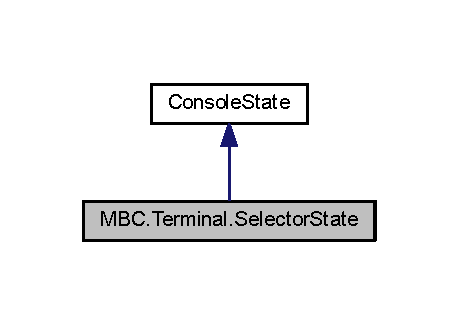
\includegraphics[width=220pt]{class_m_b_c_1_1_terminal_1_1_selector_state__inherit__graph}
\end{center}
\end{figure}


Collaboration diagram for M\-B\-C.\-Terminal.\-Selector\-State\-:\nopagebreak
\begin{figure}[H]
\begin{center}
\leavevmode
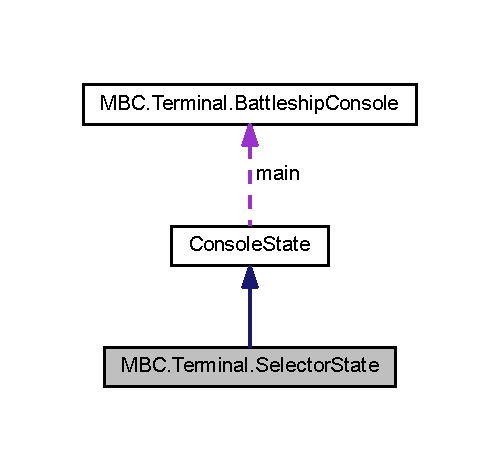
\includegraphics[width=240pt]{class_m_b_c_1_1_terminal_1_1_selector_state__coll__graph}
\end{center}
\end{figure}
\subsection*{Public Member Functions}
\begin{DoxyCompactItemize}
\item 
\hypertarget{class_m_b_c_1_1_terminal_1_1_selector_state_a64a0a29fb6288da77a4eae6fde2442b0}{{\bfseries Selector\-State} (\hyperlink{class_m_b_c_1_1_terminal_1_1_battleship_console}{Battleship\-Console} main)}\label{class_m_b_c_1_1_terminal_1_1_selector_state_a64a0a29fb6288da77a4eae6fde2442b0}

\end{DoxyCompactItemize}
\subsection*{Protected Member Functions}
\begin{DoxyCompactItemize}
\item 
\hypertarget{class_m_b_c_1_1_terminal_1_1_selector_state_a01fc2be754805e51c0f3b92d90dbe967}{override void \hyperlink{class_m_b_c_1_1_terminal_1_1_selector_state_a01fc2be754805e51c0f3b92d90dbe967}{State\-Display} ()}\label{class_m_b_c_1_1_terminal_1_1_selector_state_a01fc2be754805e51c0f3b92d90dbe967}

\begin{DoxyCompactList}\small\item\em Overridden to provide specific printing related to the subclass.\end{DoxyCompactList}\item 
override \hyperlink{class_m_b_c_1_1_terminal_1_1_console_state}{Console\-State} \hyperlink{class_m_b_c_1_1_terminal_1_1_selector_state_ad5790cf53b3c3da6269fe2faf9a0e871}{Response} (string input)
\begin{DoxyCompactList}\small\item\em Called when input is not handled by the base class.\end{DoxyCompactList}\end{DoxyCompactItemize}
\subsection*{Additional Inherited Members}


\subsection{Member Function Documentation}
\hypertarget{class_m_b_c_1_1_terminal_1_1_selector_state_ad5790cf53b3c3da6269fe2faf9a0e871}{\index{M\-B\-C\-::\-Terminal\-::\-Selector\-State@{M\-B\-C\-::\-Terminal\-::\-Selector\-State}!Response@{Response}}
\index{Response@{Response}!MBC::Terminal::SelectorState@{M\-B\-C\-::\-Terminal\-::\-Selector\-State}}
\subsubsection[{Response}]{\setlength{\rightskip}{0pt plus 5cm}override {\bf Console\-State} M\-B\-C.\-Terminal.\-Selector\-State.\-Response (
\begin{DoxyParamCaption}
\item[{string}]{input}
\end{DoxyParamCaption}
)\hspace{0.3cm}{\ttfamily [protected]}, {\ttfamily [virtual]}}}\label{class_m_b_c_1_1_terminal_1_1_selector_state_ad5790cf53b3c3da6269fe2faf9a0e871}


Called when input is not handled by the base class.


\begin{DoxyParams}{Parameters}
{\em input} & The string entered by the user\\
\hline
\end{DoxyParams}
\begin{DoxyReturn}{Returns}
The implementing class, null, or a new \hyperlink{class_m_b_c_1_1_terminal_1_1_console_state}{Console\-State} object. null will end the program.
\end{DoxyReturn}


Implements \hyperlink{class_m_b_c_1_1_terminal_1_1_console_state_a93d6eee582913a59d10348cdc8ef4248}{M\-B\-C.\-Terminal.\-Console\-State}.



Here is the call graph for this function\-:\nopagebreak
\begin{figure}[H]
\begin{center}
\leavevmode
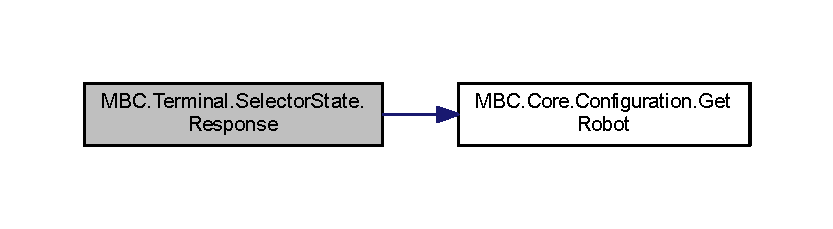
\includegraphics[width=350pt]{class_m_b_c_1_1_terminal_1_1_selector_state_ad5790cf53b3c3da6269fe2faf9a0e871_cgraph}
\end{center}
\end{figure}




The documentation for this class was generated from the following file\-:\begin{DoxyCompactItemize}
\item 
M\-B\-C Terminal/Selector\-State.\-cs\end{DoxyCompactItemize}

\hypertarget{class_m_b_c_1_1_core_1_1_ship}{\section{M\-B\-C.\-Core.\-Ship Class Reference}
\label{class_m_b_c_1_1_core_1_1_ship}\index{M\-B\-C.\-Core.\-Ship@{M\-B\-C.\-Core.\-Ship}}
}
\subsection*{Public Member Functions}
\begin{DoxyCompactItemize}
\item 
\hypertarget{class_m_b_c_1_1_core_1_1_ship_a2728c2c36920b0b340de375008a22eff}{{\bfseries Ship} (int length)}\label{class_m_b_c_1_1_core_1_1_ship_a2728c2c36920b0b340de375008a22eff}

\item 
\hypertarget{class_m_b_c_1_1_core_1_1_ship_a89511a2e24a6ce6f3346a685f6c20b7a}{void {\bfseries Place} (Point location, Ship\-Orientation orientation)}\label{class_m_b_c_1_1_core_1_1_ship_a89511a2e24a6ce6f3346a685f6c20b7a}

\item 
\hypertarget{class_m_b_c_1_1_core_1_1_ship_afbae95e084d6daeafea95e6c246b0fd4}{bool {\bfseries Is\-Valid} (Size board\-Size)}\label{class_m_b_c_1_1_core_1_1_ship_afbae95e084d6daeafea95e6c246b0fd4}

\item 
\hypertarget{class_m_b_c_1_1_core_1_1_ship_a1adf09a6c7bead42ffb4b478bd69ff1b}{bool {\bfseries Is\-At} (Point location)}\label{class_m_b_c_1_1_core_1_1_ship_a1adf09a6c7bead42ffb4b478bd69ff1b}

\item 
\hypertarget{class_m_b_c_1_1_core_1_1_ship_ad65098b265e9fa64b8fcbe5a298b2041}{I\-Enumerable$<$ Point $>$ {\bfseries Get\-All\-Locations} ()}\label{class_m_b_c_1_1_core_1_1_ship_ad65098b265e9fa64b8fcbe5a298b2041}

\item 
\hypertarget{class_m_b_c_1_1_core_1_1_ship_ac3f8bbb63b27d60b4ea3581141cdc5f9}{bool {\bfseries Conflicts\-With} (\hyperlink{class_m_b_c_1_1_core_1_1_ship}{Ship} other\-Ship)}\label{class_m_b_c_1_1_core_1_1_ship_ac3f8bbb63b27d60b4ea3581141cdc5f9}

\item 
\hypertarget{class_m_b_c_1_1_core_1_1_ship_aebf36ec312c5d6ef5c14c095444ee769}{bool {\bfseries Is\-Sunk} (I\-Enumerable$<$ Point $>$ shots)}\label{class_m_b_c_1_1_core_1_1_ship_aebf36ec312c5d6ef5c14c095444ee769}

\end{DoxyCompactItemize}
\subsection*{Properties}
\begin{DoxyCompactItemize}
\item 
\hypertarget{class_m_b_c_1_1_core_1_1_ship_a9a7f4e721f2d4cd9391e2bc633d3ceb2}{bool {\bfseries Is\-Placed}\hspace{0.3cm}{\ttfamily  \mbox{[}get\mbox{]}}}\label{class_m_b_c_1_1_core_1_1_ship_a9a7f4e721f2d4cd9391e2bc633d3ceb2}

\item 
\hypertarget{class_m_b_c_1_1_core_1_1_ship_ac2b6713dd5e22c092ec5f772379d1c78}{Point {\bfseries Location}\hspace{0.3cm}{\ttfamily  \mbox{[}get\mbox{]}}}\label{class_m_b_c_1_1_core_1_1_ship_ac2b6713dd5e22c092ec5f772379d1c78}

\item 
\hypertarget{class_m_b_c_1_1_core_1_1_ship_afcd2ca11e40556c99330a4aa0821244a}{Ship\-Orientation {\bfseries Orientation}\hspace{0.3cm}{\ttfamily  \mbox{[}get\mbox{]}}}\label{class_m_b_c_1_1_core_1_1_ship_afcd2ca11e40556c99330a4aa0821244a}

\item 
\hypertarget{class_m_b_c_1_1_core_1_1_ship_a032a96397bef51321cec9d2ec370ffca}{int {\bfseries Length}\hspace{0.3cm}{\ttfamily  \mbox{[}get\mbox{]}}}\label{class_m_b_c_1_1_core_1_1_ship_a032a96397bef51321cec9d2ec370ffca}

\end{DoxyCompactItemize}


The documentation for this class was generated from the following file\-:\begin{DoxyCompactItemize}
\item 
Controller Plugin/Ship.\-cs\end{DoxyCompactItemize}

\hypertarget{class_m_b_c_1_1_core_1_1mbc_1_1accolades_1_1_slow}{\section{M\-B\-C.\-Core.\-mbc.\-accolades.\-Slow Class Reference}
\label{class_m_b_c_1_1_core_1_1mbc_1_1accolades_1_1_slow}\index{M\-B\-C.\-Core.\-mbc.\-accolades.\-Slow@{M\-B\-C.\-Core.\-mbc.\-accolades.\-Slow}}
}


Inheritance diagram for M\-B\-C.\-Core.\-mbc.\-accolades.\-Slow\-:\nopagebreak
\begin{figure}[H]
\begin{center}
\leavevmode
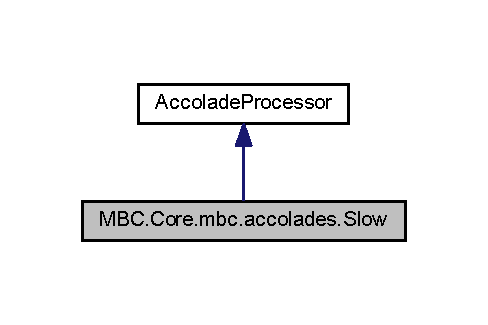
\includegraphics[width=234pt]{class_m_b_c_1_1_core_1_1mbc_1_1accolades_1_1_slow__inherit__graph}
\end{center}
\end{figure}


Collaboration diagram for M\-B\-C.\-Core.\-mbc.\-accolades.\-Slow\-:\nopagebreak
\begin{figure}[H]
\begin{center}
\leavevmode
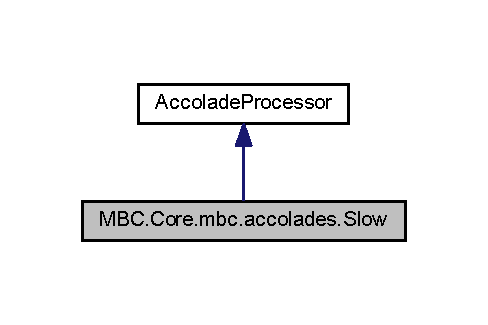
\includegraphics[width=234pt]{class_m_b_c_1_1_core_1_1mbc_1_1accolades_1_1_slow__coll__graph}
\end{center}
\end{figure}
\subsection*{Public Member Functions}
\begin{DoxyCompactItemize}
\item 
\hypertarget{class_m_b_c_1_1_core_1_1mbc_1_1accolades_1_1_slow_ae6faa3fda393b31a1dde5e0be7f40a43}{Round\-Log.\-Round\-Accolade \hyperlink{class_m_b_c_1_1_core_1_1mbc_1_1accolades_1_1_slow_ae6faa3fda393b31a1dde5e0be7f40a43}{Process} (\hyperlink{class_m_b_c_1_1_core_1_1_round_log_1_1_round_activity}{Round\-Log.\-Round\-Activity} a)}\label{class_m_b_c_1_1_core_1_1mbc_1_1accolades_1_1_slow_ae6faa3fda393b31a1dde5e0be7f40a43}

\begin{DoxyCompactList}\small\item\em Process an activity\end{DoxyCompactList}\end{DoxyCompactItemize}


The documentation for this class was generated from the following file\-:\begin{DoxyCompactItemize}
\item 
M\-B\-C Core/accolades/Slow.\-cs\end{DoxyCompactItemize}

\addcontentsline{toc}{part}{Index}
\printindex
\end{document}
